% Task C08
% Source volume: upper
% Physical scan pages: 243--294
% Printed book pages: 226--277
% Transcribe only source content; omit running headers, footers, and printed page numbers.
\chapter{微分学的应用}

% BEGIN TRANSCRIPTION

有了微分学中值定理和 Taylor 定理后，我们在函数研究方面就有了强有力的工具。本章将分专题介绍这些工具是如何应用的。虽然其中多数问题可能在过去已经遇到过，但只有在学了微分学的知识之后，我们才有条件来讨论解决这些问题的一般性方法。

§8.1 介绍求函数极限的两个主要方法——L'Hospital 法则和带 Peano 余项的 Taylor 公式。§8.2 是早已熟悉的判定函数的单调性。§8.3 是用微分学方法求函数的极值和最值。在 §8.4 中对于凸函数的基本性质作较全面的介绍。§8.5 的主题是用各种不同的方法证明不等式。§8.6 为函数作图。§8.7 是以方程求根为中心的近似计算。最后一节为学习要点和两组参考题。

\section{函数极限的计算}

\subsection{L'Hospital 法则}

从数学分析的学习开始，极限计算就是一大难题。这种状况在有了 L'Hospital 法则后才可以说有了根本的改变。由于这个法则将求不定式极限归之于简单的导数计算，而且（在条件满足时）可以连续使用，许多看似复杂的问题就可迎刃而解。关于 L'Hospital 法则的叙述、证明以及应用时的注意事项等在数学分析的教科书中都有详细的介绍，其基本思想又与 §2.4 完全相同，这里不再重复。\footnote{L'Hospital 法则的一个精彩的几何证明见 [59] 第一册的命题 2.10。}因同样的理由，也不准备举很多常规性的例题和练习题。

这里只强调指出一点，即虽然 L'Hospital 法则确实是计算极限的强有力工具，但毕竟“一花独放不是春”，初学者要学会将 L'Hospital 法则的使用与其他工具相结合，这样才能有更好的效果。这里所说的其他工具包括在前面各章中已经介绍的多种方法，如等价量代换法、变量代换法、不定式因子的分离、各种恒等变换、无穷小增量公式等，也包括在下一个小节将要介绍的带 Peano 余项的 Taylor 公式等。总之，若初学者在用 L'Hospital 法则时出现复杂的计算或甚至失败，原因往往不是 L'Hospital 法则不好，而是你对于它的认识有误。不要认为既然 L'Hospital 法则这样有力，那么其他（已经学过的）方法都可以不要了。

先看下面几个简单问题，它们在第四章中很难解决，现在用 L'Hospital 法则来做就成为容易的问题了（回顾那里的例题 4.4.5）。但从下面又可看出，这里也需要与其他工具结合。

\begin{xexample}[8.1.1]
计算极限
\[
  \lim_{x\to0}\frac{\sin x-x}{x^3}.
\]
\end{xexample}
\begin{xsolution}
用 L'Hospital 法则可计算如下：
\[
  \lim_{x\to0}\frac{\sin x-x}{x^3}
  =\lim_{x\to0}\frac{\cos x-1}{3x^2}
  =-\frac16.
\]
最后一步利用了已知的等价关系 $1-\cos x\sim\frac12x^2\ (x\to0)$。
\end{xsolution}

\begin{xexample}[8.1.2]
计算极限
\[
  \lim_{x\to0}\frac{x-\tan x}{x^3}.
\]
\end{xexample}
\begin{xsolution}
\textbf{解 1}\quad 不用其他工具，连用三次 L'Hospital 法则就可以解决问题：
\begin{align*}
  \lim_{x\to0}\frac{x-\tan x}{x^3}
  &=\lim_{x\to0}\frac{1-\operatorname{sec}^2x}{3x^2}
   =\lim_{x\to0}\frac{-2\operatorname{sec}^2x\tan x}{6x}\\
  &=-\lim_{x\to0}\frac{2\operatorname{sec}^2x\tan^2x+\operatorname{sec}^4x}{3}
   =-\frac13.
\end{align*}

\textbf{解 2}\quad 实际上用一次 L'Hospital 法则就够了：
\[
  \lim_{x\to0}\frac{x-\tan x}{x^3}
  =\lim_{x\to0}\frac{1-\operatorname{sec}^2x}{3x^2}
  =\lim_{x\to0}\frac{-\tan^2x}{3x^2}
  =-\frac13.
\]
\end{xsolution}

再举一个有多种解法的例子。

\begin{xexample}[8.1.3]
计算
\[
  \lim_{x\to0}\frac{1-\cos x^2}{x^3\sin x}.
\]
\end{xexample}
\begin{xsolution}
\textbf{解 1}\quad 直接用 L'Hospital 法则三次，得到
\begin{align*}
  \lim_{x\to0}\frac{1-\cos x^2}{x^3\sin x}
  &=\lim_{x\to0}\frac{2x\sin x^2}{3x^2\sin x+x^3\cos x}\\
  &=\lim_{x\to0}\frac{4x\cos x^2}{(3-x^2)\sin x+5x\cos x}\\
  &=\lim_{x\to0}\frac{4\cos x^2-8x^2\sin x^2}{(8-x^2)\cos x-7x\sin x}
  =\frac12.
\end{align*}

\textbf{解 2}\quad 实际上不需要微分学知识，用等价量代换法即可解决：
\begin{align*}
  \lim_{x\to0}\frac{1-\cos x^2}{x^3\sin x}
  &=\lim_{x\to0}\frac{2\sin^2\frac{x^2}{2}}{x^3\sin x}\\
  &=\lim_{x\to0}\left(\frac{\sin\frac{x^2}{2}}{\frac{x^2}{2}}\right)^2
      \left(\frac{x}{2\sin x}\right)
  =\frac12.
\end{align*}

\textbf{解 3}\quad 若利用当 $x\to0$ 时成立
\[
  \cos x^2=1-\frac{(x^2)^2}{2}+\littleo((x^2)^2),
  \qquad
  \sin x=x+\littleo(x),
\]
则就有
\begin{align*}
  \lim_{x\to0}\frac{1-\cos x^2}{x^3\sin x}
  &=\lim_{x\to0}\frac{\frac{x^4}{2}+\littleo(x^4)}{x^3(x+\littleo(x))}\\
  &=\lim_{x\to0}\frac{\frac{x^4}{2}+\littleo(x^4)}{x^4+\littleo(x^4)}
  =\lim_{x\to0}\frac{\frac12+\littleo(1)}{1+\littleo(1)}
  =\frac12.
\end{align*}
\end{xsolution}

下面是在 §2.5 计算数 $\ee$ 时留下的问题，即证明公式 (2.15) 中的等价关系。

\begin{xexample}[8.1.4]
设
\[
  \delta_n=\ee-\left(1+\frac1n\right)^n,
\]
计算极限 $\displaystyle\lim_{n\to\infty}n\delta_n$。
\end{xexample}
\begin{xsolution}
根据第四章的 Heine 归结原理（即命题 4.2.3），只要计算函数极限
\[
  \lim_{x\to0+}\frac{\ee-(1+x)^{1/x}}{x}.
\]
这是 $0/0$ 型的不定式问题。用 L'Hospital 法则，得到
\begin{align*}
  \lim_{x\to0+}\frac{\ee-(1+x)^{1/x}}{x}
  &=\lim_{x\to0+}\left\{-[(1+x)^{1/x}]\cdot
    \frac{\frac{x}{1+x}-\ln(1+x)}{x^2}\right\}\\
  &=-\ee\cdot\lim_{x\to0+}\frac{\frac{x}{1+x}-\ln(1+x)}{x^2}\\
  &=-\ee\cdot\lim_{x\to0+}
    \frac{\frac1{(1+x)^2}-\frac1{1+x}}{2x}\\
  &=-\ee\cdot\lim_{x\to0+}\frac{-1}{2(1+x)^2}
  =\frac{\ee}{2}.
\end{align*}

\begin{xremark}
实际上本题的答案就是例题 7.2.4 中的函数 $f(x)$ 的导数 $f'(0)$（乘 $-1$）。
\end{xremark}
\end{xsolution}

用 L'Hospital 法则可以对带 Peano 余项的 Taylor 公式给出新证明。

\begin{xexample}[8.1.5]
用 L'Hospital 法则证明：若 $f$ 在点 $x_0$ 存在 $f^{(n)}(x_0)$，则有
\[
  f(x)=f(x_0)+f'(x_0)(x-x_0)+\frac{f''(x_0)}{2!}(x-x_0)^2+\cdots
  +\frac{f^{(n)}(x_0)}{n!}(x-x_0)^n+\littleo((x-x_0)^n)
  \quad(x\to x_0).
\]
\end{xexample}
\begin{xproof}
如在第七章的 (7.19) 那样引进余项
\[
  r_n(x)=f(x)-\left[f(x_0)+f'(x_0)(x-x_0)+\frac{f''(x_0)}{2!}(x-x_0)^2+\cdots
  +\frac{f^{(n)}(x_0)}{n!}(x-x_0)^n\right],
\]
它满足以下的 $n+1$ 个条件：
\begin{equation}
  r_n(x_0)=0,\quad r_n'(x_0)=0,\quad\cdots,\quad r_n^{(n)}(x_0)=0.
  \tag{8.1}
  \label{eq:8.1}
\end{equation}
只需要证明
\[
  \lim_{x\to x_0}\frac{r_n(x)}{(x-x_0)^n}=0,
\]
这是 $0/0$ 型的不定式。用 L'Hospital 法则如下：
\[
  \lim_{x\to x_0}\frac{r_n(x)}{(x-x_0)^n}
  =\lim_{x\to x_0}\frac{r_n'(x)}{n(x-x_0)^{n-1}}
  =\cdots
  =\lim_{x\to x_0}\frac{r_n^{(n-1)}(x)}{n!(x-x_0)}.
\]
在以上的 $n-1$ 次应用 L'Hospital 法则中，利用了 (8.1) 中的前 $n-1$ 个条件。从条件 $r_n^{(n-1)}(x_0)=0$ 可见上面的最后一式仍然是 $0/0$ 型的不定式。但这里不能再用 L'Hospital 法则，与命题 7.2.2 中一样，从导数定义出发，即可利用条件 $r_n^{(n)}(x_0)=0$ 得到所要求证的结果。
\end{xproof}

\subsection{Taylor 公式与极限计算}

先介绍用 Taylor 公式对错误使用等价量代换法进行分析的一个例子。

\begin{xexample}[8.1.6]
根据实际教学情况，在用 L'Hospital 法则计算例题 8.1.4 中的极限时，很多学生在最后一步不再用 L'Hospital 法则，而作以下计算：
\[
  \lim_{x\to0}\frac{\frac{x}{1+x}-\ln(1+x)}{x^2}
  =\lim_{x\to0}\frac{\frac{x}{1+x}-x}{x^2}
  =\lim_{x\to0}\frac{x-(1+x)x}{(1+x)x^2}=-1,
\]
但正确答案却是 $-1/2$。问题当然出在不恰当地使用了等价量代换法。因为根据 4.4.3 小节，应当按照 (4.8) 或 (4.9) 的方式才能用等价量代换。

用 Taylor 公式进行分析就可一目了然。分子的两项可用 Taylor 公式写出为
\[
  \frac{x}{1+x}=x-x^2+\littleo(x^2)\quad(x\to0),
\]
\[
  \ln(1+x)=x-\frac12x^2+\littleo(x^2)\quad(x\to0).
\]
可见这两项相减后，$x$ 的一次项恰好对消，因此起作用的是在两个展开式中的 $x^2$ 项的系数。正确的计算为
\[
  \lim_{x\to0}\frac{\frac{x}{1+x}-\ln(1+x)}{x^2}
  =\lim_{x\to0}\frac{(x-x^2)-(x-\frac12x^2)+\littleo(x^2)}{x^2}
  =-\frac12.
\]
由此可见，前面的错误原因在于用 $x$ 替换 $\ln(1+x)$ 时太粗糙了，丢掉了在该问题中起关键作用的二次项。

从 Taylor 公式的应用来看，问题是在每一个具体场合究竟应当写出多少项？当然这需要尝试。再以上面的分子为例，将 $\ln(1+x)$ 写为 $x+\littleo(x)\ (x\to0)$，这也是 Taylor 公式，并没有错误。如果将第一项也写为 $x+\littleo(x)$，就会发现仅仅写出一次项的系数是不够的。
\end{xexample}

以上错误还说明，学生在刚学了 Taylor 公式后一般还不会在求函数极限时加以使用，在计算时仍停留在使用无穷小增量公式（也就是 $n=1$ 的带 Peano 余项的最简单的 Taylor 公式）的知识水平上。解决这个问题的方法是实践和教师的引导。

带有 Peano 余项的 Taylor 公式在求极限中有广泛的应用是不奇怪的，因为 Peano 余项本身就是对于无穷小量的一个刻画。下面是应用 Taylor 公式求极限的第一个例子（为清楚起见用 $\exp(x)$ 表示 $\ee^x$）。

\paragraph{例题 8.1.4 的解 2}
用 Taylor 公式作下列计算：
\begin{align*}
  \delta_n
  &=\ee-\left(1+\frac1n\right)^n
   =\ee-\exp\left[n\ln\left(1+\frac1n\right)\right]\\
  &=\ee-\exp\left[n\left(\frac1n-\frac1{2n^2}+\bigO\left(\frac1{n^3}\right)\right)\right]\\
  &=\ee-\exp\left[1-\frac1{2n}+\bigO\left(\frac1{n^2}\right)\right]\\
  &=\ee\left(1-\exp\left[-\frac1{2n}+\bigO\left(\frac1{n^2}\right)\right]\right)\\
  &=\ee\left[1-\left(1-\frac1{2n}+\bigO\left(\frac1{n^2}\right)\right)\right]\\
  &=\frac{\ee}{2n}+\bigO\left(\frac1{n^2}\right).
\end{align*}
可见
\[
  \lim_{n\to\infty}n\delta_n=\frac{\ee}{2}.
\]
\begin{xremark}
例题 7.2.4 已经提供了本题的一种解法，实质上与此相同。此外，本章第一组参考题 6 又提供了另一个解法。
\end{xremark}

在用 L'Hospital 法则时，如果逐次求导运算会使表达式变得很复杂，则往往不如用 Taylor 公式或结合其他工具为好。

\begin{xexample}[8.1.7]
求
\[
  \lim_{x\to0}\frac{1-(\cos x)^{\sin x}}{x^3}.
\]
\end{xexample}
\begin{xsolution}
记所求的极限为 $I$，写出分子的 Maclaurin 公式：
\begin{align*}
  1-(\cos x)^{\sin x}
  &=1-\ee^{\sin x\ln\cos x}\\
  &=1-[1+\sin x\ln\cos x+\littleo(\sin x\ln\cos x)]\\
  &=-\sin x\ln\cos x+\littleo(\sin x\ln\cos x)\quad(x\to0),
\end{align*}
然后如下计算即可得到答案：
\begin{align*}
  I
  &=\lim_{x\to0}\frac{-\sin x\ln\cos x}{x^3}
   =\lim_{x\to0}\frac{-\ln\cos x}{x^2}\\
  &=\lim_{x\to0}\frac{-\ln[1+(-\frac{x^2}{2}+\littleo(x^3))]}{x^2}\\
  &=\lim_{x\to0}\frac{\frac{x^2}{2}+\littleo(x^3)+\littleo(x^2)}{x^2}
   =\frac12.
\end{align*}
\end{xsolution}

在下一个例题的几种解法中我们可以看到各种工具的结合使用。

\begin{xexample}[8.1.8]
求极限
\[
  \lim_{x\to0}\frac{\cos(\sin x)-\cos x}{x^4}.
\]
\end{xexample}
\begin{xsolution}
\textbf{解 1}\quad 可以看出只要计算分子的 Maclaurin 展开式直到 $x^4$ 项即可：
\begin{align*}
  \cos(\sin x)-\cos x
  &=1-\frac1{2!}(\sin x)^2+\frac1{4!}(\sin x)^4
    -\left(1-\frac1{2!}x^2+\frac1{4!}x^4\right)+\littleo(x^5)\\
  &=-\frac12\left(x-\frac16x^3\right)^2+\frac1{24}x^4+\frac12x^2-\frac1{24}x^4+\littleo(x^5)\\
  &=-\frac12\left(x^2-\frac13x^4\right)+\frac12x^2+\littleo(x^5)\\
  &=\frac16x^4+\littleo(x^5)\quad(x\to0),
\end{align*}
因此所求的极限为 $1/6$。

\textbf{解 2}\quad 在写出 $\cos(\sin x)-\cos x$ 的展开式后，可以看出只要计算如下：
\begin{align*}
  \lim_{x\to0}\frac{\cos(\sin x)-\cos x}{x^4}
  &=\lim_{x\to0}\left(\frac12\cdot\frac{x^2-\sin^2x}{x^4}\right)\\
  &=\frac12\lim_{x\to0}\left(\frac{x+\sin x}{x}\cdot\frac{x-\sin x}{x^3}\right)
  =\frac16.
\end{align*}

\textbf{解 3}\quad 利用分子的特殊形式，应用 Lagrange 中值定理即可得到
\[
  \cos(\sin x)-\cos x=-\sin\xi(\sin x-x),
\]
其中 $\xi$ 在 $x$ 与 $\sin x$ 之间。因此就可以计算如下：
\begin{align*}
  \lim_{x\to0}\frac{\cos(\sin x)-\cos x}{x^4}
  &=\lim_{x\to0}\frac{-\sin\xi(\sin x-x)}{x^4}\\
  &=-\lim_{x\to0}\left(\frac{\sin\xi}{\xi}\cdot\frac{\xi}{x}\cdot\frac{\sin x-x}{x^3}\right)
  =\frac16.
\end{align*}

\textbf{解 4}\quad 本题也可以用三角函数的和差化积公式来做，计算如下：
\begin{align*}
  \lim_{x\to0}\frac{\cos(\sin x)-\cos x}{x^4}
  &=\lim_{x\to0}\left[-\frac1{x^4}\cdot2\sin\left(\frac{\sin x-x}{2}\right)
  \cdot\sin\left(\frac{\sin x+x}{2}\right)\right]\\
  &=-2\lim_{x\to0}\left(\frac1{x^4}\cdot\frac{\sin x-x}{2}\cdot\frac{\sin x+x}{2}\right)\\
  &=-\lim_{x\to0}\frac{\sin x-x}{x^3}=\frac16.
\end{align*}
注意这里使用了多次等价量代换，使问题大大简化了。
\end{xsolution}

\begin{xexample}[8.1.9]
设函数 $f$ 满足条件 $f(0)=0$，且存在 $f''(0)$，证明：函数
\[
  g(x)=
  \begin{cases}
    \dfrac{f(x)}{x}, & x\ne0,\\
    f'(0), & x=0
  \end{cases}
\]
的导函数 $g'$ 在 $x=0$ 处连续，且 $g'(0)=\dfrac12f''(0)$。
\end{xexample}
\begin{xsolution}
这时 $f$ 在 $x=0$ 的某邻域上可微，因此当 $x\ne0$ 时可按定义求出
\begin{equation}
  g'(x)=\frac{f'(x)x-f(x)}{x^2}.
  \tag{8.2}
  \label{eq:8.2}
\end{equation}
余下只有一个问题，即证明 $g'(0)=\frac12f''(0)$ 且 $\lim_{x\to0}g'(x)=g'(0)$。

应用 7.1.2 小节的导数极限定理，只要证明：(1) $g$ 在 $x=0$ 处连续；(2) $g'$ 在 $x=0$ 处有极限，并求出此极限。（若不用导数极限定理，则需另行计算 $g'(0)$。）

(1) 从 $g$ 的定义即可得到
\[
  \lim_{x\to0}g(x)=\lim_{x\to0}\frac{f(x)}{x}
  =\lim_{x\to0}\frac{f(x)-f(0)}x=f'(0)=g(0).
\]

(2) 利用带 Peano 余项的 Maclaurin 公式：
\[
  f(x)=f'(0)x+\frac12f''(0)x^2+\littleo(x^2)\quad(x\to0),
\]
\[
  f'(x)=f'(0)+f''(0)x+\littleo(x)\quad(x\to0),
\]
将它们代入 (8.2)，就在 $x\ne0$ 时有
\[
  g'(x)=\frac{(f'(0)+f''(0)x)x-(f'(0)x+\frac12f''(0)x^2)+\littleo(x^2)}{x^2}
  =\frac12f''(0)+\littleo(1)\quad(x\to0).
\]
因此存在极限 $\lim_{x\to0}g'(x)=\frac12f''(0)$，再应用导数极限定理即得所要的结论。

\begin{xremark}
\textbf{注 1}\quad 比较 $f$ 和 $g$ 的 Maclaurin 展开式：
\[
  f(x)=f'(0)x+\frac{f''(0)}2x^2+\littleo(x^2)\quad(x\to0),
\]
\[
  g(x)=f'(0)+\frac{f''(0)}2x+\littleo(x)\quad(x\to0),
\]
可以发现，后一个公式可以由前一个除以 $x$ 得到，恰与 $x\ne0$ 时 $g(x)$ 的定义一致。但是在证明 $g(0)=f'(0)$ 和 $g'(0)=\frac12f''(0)$ 之前，当然还不知道由这样的形式运算得到的结果是否是 $g$ 的 Maclaurin 展开式。因此可以认为，本例题的意义就在于对这样的形式运算作出了严格证明。

\textbf{注 2}\quad 这个例题的结论可以推广。只要多次应用导数极限定理，就可以证明：若 $f(0)=0$，且存在 $f^{(n+1)}(0)$，则上述 $g(x)$ 的 $n$ 阶导函数 $g^{(n)}$ 在 $x=0$ 处连续，且
\[
  g^{(n)}(0)=\frac{f^{(n+1)}(0)}{n+1}.
\]
（这将作为本章的第二组参考题 2。）

\textbf{注 3}\quad 应用上述推广，就可以为上一章的例题 7.2.3 和 7.2.4 中的计算提供理论根据。这里的结果可以简述为：如果 $f(x)$ 满足 $f(0)=0$，又存在 $f^{(n+1)}(0)$，则如下定义的函数：
\[
  g(x)=
  \begin{cases}
    \dfrac{f(x)}{x}, & x\ne0,\\
    f'(0), & x=0
  \end{cases}
\]
在 $x=0$ 处存在 $g^{(n)}(0)$，且有 Maclaurin 展开式：
\[
  g(x)=f'(0)+f''(0)x+\frac{f'''(0)}{2!}x^2+\cdots
  +\frac{f^{(n+1)}(0)}{(n+1)!}x^n+\littleo(x^n)\quad(x\to0).
\]
因此，形式上这个展开式可以从 $f$ 的 Maclaurin 展开式除以 $x$ 得到。在例题 7.2.3 和 7.2.4 中对于 $\sin x$ 和 $\ln(1+x)$ 就是这样做的，但当时没有能够证明其合理性。
\end{xremark}
\end{xsolution}

下一个例题与例题 2.4.2 类似，但需要用到 Taylor 公式的知识才能解决。

\begin{xexample}[8.1.10]
设 $x_0\in(0,\frac\pi2)$，$x_n=\sin x_{n-1}$，$n\in\NN_+$，证明：
\[
  x_n\sim\sqrt{\frac3n}\quad(n\to\infty).
\]
\end{xexample}
\begin{xproof}
数列 $\{x_n\}$ 为严格单调减少数列，收敛于 0（请读者补充证明）。以下用 Stolz 定理计算：
\begin{align*}
  \lim_{n\to\infty}nx_n^2
  &=\lim_{n\to\infty}\frac{n}{1/x_n^2}
   =\lim_{n\to\infty}\frac1{\frac1{x_{n+1}^2}-\frac1{x_n^2}}\\
  &=\lim_{n\to\infty}\frac{x_n^2x_{n+1}^2}{x_n^2-x_{n+1}^2}
   =\lim_{n\to\infty}\frac{x_n^2\sin^2x_n}{\frac13x_n^4+\littleo(x_n^5)}
   =3,
\end{align*}
在其中用了 $x_{n+1}=\sin x_n=x_n-\frac16x_n^3+\littleo(x_n^4)$。

\begin{center}
  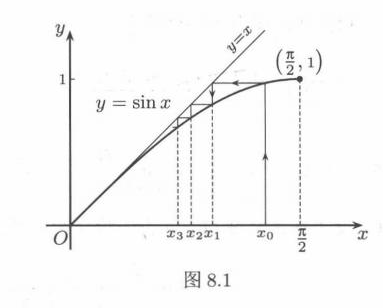
\includegraphics[width=.48\linewidth]{figures/upper/ch08/fig-8-1.png}
\end{center}

\begin{xremark}
在图 8.1 上用蛛网工作法（见 2.6.2 小节）作出了数列的前几项，可以看出数列 $\{x_n\}$ 收敛于 0 一定很慢。本题的结果对此作出了渐近的刻画。
\end{xremark}
\end{xproof}

\subsection{练习题}

\begin{xexercise}[1]
以下几个函数极限均不宜用 L'Hospital 法则，为什么？
  \begin{enumerate}[label=(\arabic*)]
    \item $\displaystyle\lim_{x\to1}\frac{x}{x+1}$；
    \item $\displaystyle\lim_{x\to+\infty}\frac{x+\sin x}{x-\sin x}$；
    \item $\displaystyle\lim_{x\to+\infty}\frac{\ee^x+\ee^{-x}}{\ee^x-\ee^{-x}}$；
    \item $\displaystyle\lim_{x\to+\infty}\frac{x}{\sqrt{1+x^2}}$。
  \end{enumerate}
\end{xexercise}
\begin{xsolution}
逐题检查 L'Hospital 法则的适用条件及求导后的表达式。
\begin{enumerate}[label=(\arabic*)]
  \item 当 $x\to1$ 时原式趋于 $1/2$，既不是 $0/0$ 型也不是 $\infty/\infty$ 型，因此不能使用 L'Hospital 法则。

  \item 原式虽为 $\infty/\infty$ 型，但求导后得到
  \[
    \frac{1+\cos x}{1-\cos x}.
  \]
  该比值在 $x\to+\infty$ 时没有极限，而且分母导数 $1-\cos x$ 在任意远处仍有零点，故 L'Hospital 法则不能给出所求极限。直接同除以 $x$ 即得
  \[
    \frac{1+\sin x/x}{1-\sin x/x}\to1.
  \]

  \item 求导后得到
  \[
    \frac{\ee^x-\ee^{-x}}{\ee^x+\ee^{-x}},
  \]
  恰为原比值的倒数；若继续求导又回到原式，因此单靠反复使用 L'Hospital 法则只会循环。直接同除以 $\ee^x$ 得
  \[
    \frac{1+\ee^{-2x}}{1-\ee^{-2x}}\to1.
  \]

  \item 求导后得到
  \[
    \frac{1}{x/\sqrt{1+x^2}}=\frac{\sqrt{1+x^2}}x,
  \]
  仍是原比值的倒数，因而同样形成循环。直接同除以 $x$：
  \[
    \frac{x}{\sqrt{1+x^2}}=\frac1{\sqrt{1+x^{-2}}}\to1.
  \]
\end{enumerate}
\end{xsolution}


\begin{xexercise}[2]
求下列极限：
  \begin{enumerate}[label=(\arabic*)]
    \item $\displaystyle\lim_{x\to0}\frac{a^{x^2}-b^{x^2}}{(a^x-b^x)^2}$；
    \item $\displaystyle\lim_{x\to+\infty}\left[\left(x^3-x^2+\frac x2\right)\ee^{1/x}-\sqrt{1+x^6}\right]$；
    \item $\displaystyle\lim_{x\to0+}\left(\ln\frac1x\right)^x$；
    \item $\displaystyle\lim_{x\to+\infty}\left(\frac\pi2-\arctan x\right)^{1/\ln x}$。
  \end{enumerate}
\end{xexercise}
\begin{xsolution}
\begin{enumerate}[label=(\arabic*)]
  \item 设 $a,b>0$ 且 $a\ne b$。当 $x\to0$ 时
  \[
    a^{x^2}-b^{x^2}=x^2(\ln a-\ln b)+\littleo(x^2),
  \]
  而
  \[
    a^x-b^x=x(\ln a-\ln b)+\littleo(x).
  \]
  因而
  \[
    \lim_{x\to0}\frac{a^{x^2}-b^{x^2}}{(a^x-b^x)^2}
    =\frac1{\ln a-\ln b}=\frac1{\ln(a/b)}.
  \]
  若 $a=b$，原分母恒为零，原式没有通常意义。

  \item 令 $t=1/x$。有
  \[
    (1-t+\tfrac12t^2)\ee^t=1+\frac16t^3+\bigO(t^4),
  \]
  故
  \[
    \left(x^3-x^2+\frac x2\right)\ee^{1/x}
    =x^3+\frac16+\bigO(x^{-1}).
  \]
  又
  \[
    \sqrt{1+x^6}=x^3\sqrt{1+x^{-6}}=x^3+\bigO(x^{-3}).
  \]
  所以极限为 $1/6$。

  \item 取对数：
  \[
    \ln\left(\ln\frac1x\right)^x=x\ln\ln\frac1x.
  \]
  令 $t=\ln(1/x)\to+\infty$，则右端为 $\ee^{-t}\ln t\to0$，故极限为 $1$。

  \item 因 $x>0$ 时 $\frac\pi2-\arctan x=\arctan(1/x)\sim1/x$，故
  \[
    \ln\left(\frac\pi2-\arctan x\right)^{1/\ln x}
    =\frac{\ln(\frac\pi2-\arctan x)}{\ln x}\to-1.
  \]
  因此极限为 $\ee^{-1}$。
\end{enumerate}
\end{xsolution}


\begin{xexercise}[3]
确定 $a,b$，使得当 $x\to0$ 时，下列函数为尽可能高阶的无穷小量：
  \begin{enumerate}[label=(\arabic*)]
    \item $f(x)=x-(a+b\cos x)\sin x$；
    \item $f(x)=\ee^x-\dfrac{1+ax}{1+bx}$；
    \item $f(x)=\cot x-\dfrac{1+ax^2}{x+bx^3}$；
    \item $f(x)=\cos x-\dfrac{1+ax^2}{1+bx^2}$。
  \end{enumerate}
\end{xexercise}
\begin{xsolution}
逐项比较 Maclaurin 展开式的低阶系数即可。
\begin{enumerate}[label=(\arabic*)]
  \item
  \[
    (a+b\cos x)\sin x
    =(a+b)x+\left(-\frac{a+b}{6}-\frac b2\right)x^3
    +\left(\frac{a+b}{120}+\frac b8\right)x^5+\bigO(x^7).
  \]
  令一次、三次项在 $x-(a+b\cos x)\sin x$ 中消失，得
  \[
    a+b=1,\qquad \frac16+\frac b2=0,
  \]
  即
  \[
    a=\frac43,\qquad b=-\frac13.
  \]
  此时 $f(x)=\frac1{30}x^5+\bigO(x^7)$，故最高可做到五阶。

  \item
  \[
    \frac{1+ax}{1+bx}
    =1+(a-b)x-b(a-b)x^2+b^2(a-b)x^3+\bigO(x^4).
  \]
  与 $\ee^x$ 比较，令一次、二次项相同：
  \[
    a-b=1,\qquad -b=\frac12.
  \]
  因而
  \[
    a=\frac12,\qquad b=-\frac12.
  \]
  此时三次项之差为 $1/6-1/4=-1/12$，故 $f(x)=-x^3/12+\bigO(x^4)$。

  \item
  \[
    \frac{1+ax^2}{x+bx^3}
    =\frac1x+(a-b)x-b(a-b)x^3+b^2(a-b)x^5+\bigO(x^7),
  \]
  而
  \[
    \cot x=\frac1x-\frac x3-\frac{x^3}{45}-\frac{2x^5}{945}+\bigO(x^7).
  \]
  令 $a-b=-1/3$、$-b(a-b)=-1/45$，得到
  \[
    b=-\frac1{15},\qquad a=-\frac25.
  \]
  此时五次项之差为 $-1/1575$，所以最高为五阶无穷小。

  \item
  \[
    \frac{1+ax^2}{1+bx^2}
    =1+(a-b)x^2-b(a-b)x^4+b^2(a-b)x^6+\bigO(x^8).
  \]
  与
  \[
    \cos x=1-\frac{x^2}{2}+\frac{x^4}{24}-\frac{x^6}{720}+\bigO(x^8)
  \]
  比较，得
  \[
    a-b=-\frac12,\qquad \frac b2=\frac1{24},
  \]
  即
  \[
    b=\frac1{12},\qquad a=-\frac5{12}.
  \]
  此时 $f(x)=x^6/480+\bigO(x^8)$，故最高为六阶。
\end{enumerate}
\end{xsolution}


\begin{xexercise}[4]
应用 Taylor 公式求下列极限：
  \begin{enumerate}[label=(\arabic*)]
    \item $\displaystyle\lim_{x\to0}\left(\frac1x-\frac1{\sin x}\right)$；
    \item $\displaystyle\lim_{x\to0}\frac{\ee^{x^3}-1-x^3}{\sin^6 2x}$；
    \item $\displaystyle\lim_{n\to\infty}n^2\ln\left(n\sin\frac1n\right)$；
    \item $\displaystyle\lim_{n\to\infty}(-1)^n n\sin\bigl(\sqrt{n^2+2}\,\pi\bigr)$；
    \item $\displaystyle\lim_{x\to0}\frac{\sin(\tan x)-\tan(\sin x)}{x^7}$；
    \item $\displaystyle\lim_{x\to0}\frac{x\sin(\sin x)-\sin^2x}{x^6}$。
  \end{enumerate}
\end{xexercise}
\begin{xsolution}
\begin{enumerate}[label=(\arabic*)]
  \item 由 $\sin x=x-x^3/6+\bigO(x^5)$，
  \[
    \frac1x-\frac1{\sin x}
    =\frac{\sin x-x}{x\sin x}\sim-\frac x6\to0.
  \]

  \item
  \[
    \ee^{x^3}-1-x^3=\frac12x^6+\bigO(x^9),\qquad
    \sin^6 2x=64x^6+\littleo(x^6),
  \]
  故极限为 $1/128$。

  \item
  \[
    n\sin\frac1n=1-\frac1{6n^2}+\bigO(n^{-4}),
  \]
  因而
  \[
    n^2\ln\left(n\sin\frac1n\right)
    =n^2\left(-\frac1{6n^2}+\bigO(n^{-4})\right)\to-\frac16.
  \]

  \item
  \[
    \sqrt{n^2+2}\,\pi
    =n\pi+\frac\pi n+\bigO(n^{-3}).
  \]
  因此
  \[
    (-1)^n n\sin(\sqrt{n^2+2}\,\pi)
    =n\sin\left(\frac\pi n+\bigO(n^{-3})\right)\to\pi.
  \]

  \item 展开到七次项可得
  \[
    \sin(\tan x)-\tan(\sin x)=-\frac1{30}x^7+\bigO(x^9),
  \]
  故极限为 $-1/30$。

  \item 展开到六次项可得
  \[
    x\sin(\sin x)-\sin^2x=\frac1{18}x^6+\bigO(x^8),
  \]
  故极限为 $1/18$。
\end{enumerate}
\end{xsolution}


\begin{xexercise}[5]
设存在 $f''(a)$，证明：
  \[
    \lim_{h\to0}\frac{f(a+2h)-2f(a+h)+f(a)}{h^2}=f''(a).
  \]
\end{xexercise}
\begin{xsolution}
由 $f''(a)$ 存在，
\[
  f(a+h)=f(a)+f'(a)h+\frac12f''(a)h^2+\littleo(h^2),
\]
\[
  f(a+2h)=f(a)+2f'(a)h+2f''(a)h^2+\littleo(h^2).
\]
相减后
\[
  f(a+2h)-2f(a+h)+f(a)=f''(a)h^2+\littleo(h^2),
\]
除以 $h^2$ 并令 $h\to0$ 即得结论。
\end{xsolution}


\begin{xexercise}[6]
设 $f$ 在某邻域 $O(x_0)$ 上二阶连续可微，$f'(x_0)\ne0$，$f(x)\ne f(x_0)$，$\forall x\ne x_0$。求
  \[
    \lim_{x\to x_0}\left[\frac1{f(x)-f(x_0)}-\frac1{f'(x_0)(x-x_0)}\right].
  \]
\end{xexercise}
\begin{xsolution}
记 $t=x-x_0$，$A=f'(x_0)\ne0$，$B=f''(x_0)/2$。二阶 Taylor 公式给出
\[
  f(x)-f(x_0)=At+Bt^2+\littleo(t^2).
\]
于是
\begin{align*}
  &\frac1{f(x)-f(x_0)}-\frac1{f'(x_0)(x-x_0)}\\
  &\quad=\frac{At-[At+Bt^2+\littleo(t^2)]}
  {At[At+Bt^2+\littleo(t^2)]}
  \to-\frac{B}{A^2}.
\end{align*}
故所求极限为
\[
  -\frac{f''(x_0)}{2[f'(x_0)]^2}.
\]
\end{xsolution}


\begin{xexercise}[7]
设 $f$ 在 $[0,+\infty)$ 上二阶连续可微，且 $f''(x)>0$，$f(0)=f'(0)=0$。试求极限
  \[
    \lim_{x\to0+}\frac{xf(u)}{uf(x)},
  \]
  其中 $u$ 是函数 $f$ 的图像在点 $(x,f(x))$ 处的切线在 $x$ 轴上的截距。
\end{xexercise}
\begin{xsolution}
切线方程为
\[
  Y-f(x)=f'(x)(X-x),
\]
故其 $x$ 轴截距
\[
  u=x-\frac{f(x)}{f'(x)}.
\]
记 $c=f''(0)>0$。当 $x\to0+$ 时
\[
  f(x)=\frac c2x^2+\littleo(x^2),\qquad
  f'(x)=cx+\littleo(x),
\]
所以
\[
  u=\frac x2+\littleo(x),\qquad \frac ux\to\frac12.
\]
又 $u\to0+$，故
\[
  \frac{f(u)}{f(x)}\sim\frac{u^2}{x^2}.
\]
从而
\[
  \frac{x f(u)}{u f(x)}\sim\frac ux\to\frac12.
\]
\end{xsolution}


\begin{xexercise}[8]
令
  \[
    f(x)=\lim_{n\to\infty}n^x\left[\left(1+\frac1{n+1}\right)^{n+1}-\left(1+\frac1n\right)^n\right],
  \]
  确定其定义域和值域。
\end{xexercise}
\begin{xsolution}
记
\[
  a_n=\left(1+\frac1n\right)^n.
\]
由
\[
  n\ln\left(1+\frac1n\right)
  =1-\frac1{2n}+\frac1{3n^2}+\bigO(n^{-3})
\]
得到
\[
  a_n=\ee\left(1-\frac1{2n}+\frac{11}{24n^2}+\bigO(n^{-3})\right).
\]
因此
\[
  a_{n+1}-a_n=\frac{\ee}{2n^2}+\bigO(n^{-3}).
\]
于是
\[
  n^x(a_{n+1}-a_n)
  =\frac\ee2 n^{x-2}(1+\littleo(1)).
\]
按通常实值函数的定义，极限有限的 $x$ 恰为 $x\le2$，且
\[
  f(x)=
  \begin{cases}
    0,&x<2,\\
    \ee/2,&x=2.
  \end{cases}
\]
故定义域为 $(-\infty,2]$，值域为 $\{0,\ee/2\}$。若允许扩充实数值，则 $x>2$ 时极限为 $+\infty$。
\end{xsolution}


\begin{xexercise}[9]
设 $x_1>0$，$x_{n+1}=\ln(1+x_n)$，$n\in\NN_+$，证明：$\displaystyle\lim_{n\to\infty}nx_n=2$。
\end{xexercise}
\begin{xsolution}
因 $0<\ln(1+t)<t$（$t>0$），有 $0<x_{n+1}<x_n$，故 $x_n\to L\ge0$。令极限进入递推式得 $L=\ln(1+L)$，所以 $L=0$。

考察 $1/x_n$，有
\begin{align*}
  \frac1{x_{n+1}}-\frac1{x_n}
  &=\frac{x_n-\ln(1+x_n)}{x_n\ln(1+x_n)}\\
  &\to\frac12,
\end{align*}
其中用了
\[
  \ln(1+x)=x-\frac{x^2}{2}+\littleo(x^2).
\]
由 Stolz 定理，
\[
  \lim_{n\to\infty}\frac{1/x_n}{n}=\frac12,
\]
即
\[
  \boxed{\lim_{n\to\infty}nx_n=2}.
\]
\end{xsolution}


\begin{xexercise}[10]
设 $x_0=\ln a$，$a>0$，$x_n=\displaystyle\sum_{k=0}^{n-1}\ln(a-x_k)$，$n\in\NN_+$，求 $\displaystyle\lim_{n\to\infty}x_n$。
\end{xexercise}
\begin{xsolution}
由定义
\[
  x_{n+1}=x_n+\ln(a-x_n).
\]
令 $y_n=a-x_n$，则
\[
  y_{n+1}=y_n-\ln y_n,
  \qquad y_0=a-\ln a.
\]
由基本不等式 $\ln a\le a-1$ 得 $y_0\ge1$。若 $y_n>1$，则
\[
  1<y_n-\ln y_n<y_n,
\]
其中左边由函数 $u-\ln u$ 在 $u\ge1$ 上递增且在 $u=1$ 取值 1 得到。因此 $\{y_n\}$ 单调减少且以下界 1 有界；若其极限为 $L$，则
\[
  L=L-\ln L,
\]
故 $L=1$。当 $a=1$ 时从一开始即 $y_n=1$。综上
\[
  \boxed{\lim_{n\to\infty}x_n=a-1}.
\]
\end{xsolution}


\section{函数的单调性}

设函数 $f\in C(I)$，在 $I$ 的内点处处可微，则有以下结论。

1. $f$ 为区间 $I$ 上的单调函数的充分必要条件是导数不变号。

2. $f$ 为区间 $I$ 上的严格单调函数的充分必要条件是除了导数不变号外，还在集合 $\{x\in I\mid f'(x)=0\}$ 中不包含任何长度大于零的区间。

证明的方法是用 Lagrange 中值定理。这在教科书中都有，不再重复。

从数列极限和函数极限的学习开始，单调性就一直起着重要的作用。现在以导数为工具，给出了判定单调性的新的有效方法，可以说解决了函数研究中的一个基本问题。搞清了函数的不同单调区间，也就知道了函数图像的上升与下降，这对解决许多问题都是有帮助的。

\subsection{例题}

虽然函数的单调性与导数有如上所说的密切关系，但仅仅由一个点上的导数符号不能得出单调性。请将下一个例题与命题 7.1.1 联系起来考虑这个问题。

\begin{xexample}[8.2.1]
问：由函数在一个点上的导数符号大于（小于）0 能否推出函数在该点的一个充分小的邻域上为单调？
\end{xexample}
\begin{xsolution}
答案是不能。举例如下：令
\[
  f(x)=
  \begin{cases}
    x+2x^2\sin\dfrac1x, & x\ne0,\\
    0, & x=0.
  \end{cases}
\]
则易求出 $f'(0)=1>0$。又可以求出当 $x\ne0$ 时的导函数表达式为
\[
  f'(x)=1+4x\sin\frac1x-2\cos\frac1x.
\]
取 $x=1/(n\pi)$，则有
\[
  f'\left(\frac1{n\pi}\right)=1-2(-1)^n,
\]
可见在 $x=0$ 的任意邻近导函数 $f'(x)$ 都不保号，因此在 $x=0$ 的每个邻域上 $f$ 都不是单调的（该函数在 $x>0$ 部分的图像见图 8.2(a)）。
\end{xsolution}

\begin{xremark}
在任何一个区间上不单调的连续函数和可微函数都是存在的（见 [57]）。
\end{xremark}

\begin{xexample}[8.2.2]
问：函数在其极值点的每一侧邻近是否一定具有单调性？
\end{xexample}
\begin{xsolution}
答案是不一定。举例如下：令
\[
  f(x)=
  \begin{cases}
    0, & x=0,\\
    -x^2\left(2+\sin\dfrac1x\right), & x\ne0,
  \end{cases}
\]
则 $f$ 在 $x=0$ 处取到极大值 0。从不等式
\[
  -3x^2\le f(x)\le -x^2
\]
即可求出 $f'(0)=0$。但当 $x\ne0$ 时
\[
  f'(x)=-4x-2x\sin\frac1x+\cos\frac1x,
\]
因此在极值点 $x=0$ 两侧的任意邻近都不可能是单调的（见图 8.2(b)）。
\end{xsolution}

\begin{center}
  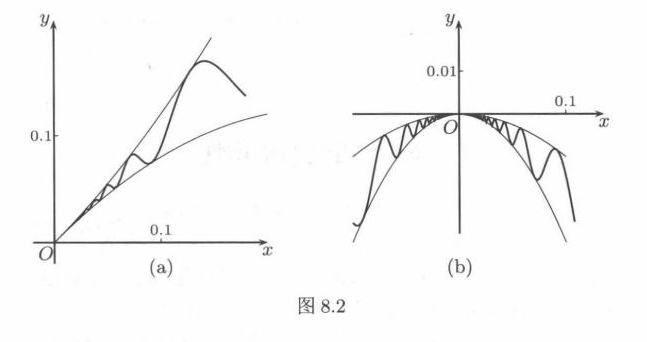
\includegraphics[width=.72\linewidth]{figures/upper/ch08/fig-8-2.png}
\end{center}

\begin{xexample}[8.2.3]
设函数
\[
  f(x)=\left(1+\frac1x\right)^{x+\alpha},
\]
证明：当 $\alpha\ge\frac12$ 时，$f$ 于 $x>0$ 时严格单调减少；而当 $\alpha<\frac12$ 时，则 $f$ 于 $x$ 充分大时严格单调增加。
\end{xexample}
\begin{xproof}
用对数求导法，可以写出
\[
  f'(x)=f(x)\left[\ln\left(1+\frac1x\right)-\frac{x+\alpha}{x^2+x}\right].
\]
将上式右边记为 $f(x)\cdot u(x)$，则 $f'$ 与 $u$ 同号。由于有
\[
  \lim_{x\to+\infty}u(x)=0,
\]
只要观察 $u$ 是否单调即可判定其符号。计算得到
\[
  u'(x)=\frac{\alpha+(2\alpha-1)x}{x^2(1+x)^2}.
\]
可见当 $\alpha\ge\frac12$ 和 $x>0$ 时有 $u'(x)>0$，因此 $u$ 为严格单调增加函数，所以当 $x>0$ 时 $u(x)<0$ 成立。这保证了 $f$ 在 $x>0$ 时严格单调减少。当 $\alpha<\frac12$ 时，则至少在 $x$ 充分大时 $u'(x)<0$，所以有 $u(x)>0$。这保证了函数 $f$ 在 $x$ 充分大时严格单调增加。
\end{xproof}

将单调性分析与连续函数的零点存在定理相结合，就可以确定方程的根的个数。以下是在一维动力系统的研究中出现的一个代数方程。

\begin{xexample}[8.2.4]
证明：对每个正整数 $n$，方程
\[
  x^{n+2}-2x^n-1=0
\]
只有唯一正根。
\end{xexample}
\begin{xproof}
记方程左边的表达式为 $f(x)$。从 $f(\sqrt2)=-1$ 和 $f(+\infty)=+\infty$ 可见方程有大于 $\sqrt2$ 的正根。为了知道 $f$ 的单调性，求导后得到
\[
  f'(x)=(n+2)x^{n+1}-2nx^{n-1}
  =(n+2)x^{n-1}\left(x^2-\frac{2n}{n+2}\right).
\]
因此函数 $f$ 在点
\[
  \xi=\sqrt{\frac{2n}{n+2}}\ (<\sqrt2)
\]
的导数值为 0。函数 $f$ 在区间 $[0,\xi]$ 上严格单调减少，而在区间 $[\xi,+\infty)$ 上严格单调增加。又从 $f(0)=-1$，就知道 $f(x)=0$ 除了上述大于 $\sqrt2$ 的一个正根外没有其他正根。
\end{xproof}

\begin{xexample}[8.2.5]
设 $a>0$，确定方程
\[
  f(x)=ax-\ln x=0
\]
恰有两个正根的条件。
\end{xexample}
\begin{xsolution}
从 $f'(x)=a-1/x$ 可见在 $(0,a^{-1}]$ 上 $f$ 严格单调减少，而在 $[a^{-1},+\infty)$ 上 $f$ 严格单调增加。又由于
\[
  f(0+)=+\infty,\qquad
  f(+\infty)=\lim_{x\to+\infty}x\left(a-\frac{\ln x}{x}\right)=+\infty,
\]
可见方程 $f(x)=0$ 有两个正根的条件是
\[
  f\left(\frac1a\right)=1-\ln\frac1a<0.
\]
由此可以确定 $a$ 应当满足条件 $a<1/\ee$。
\end{xsolution}

\subsection{练习题}

\begin{xexercise}[1]
问：单调函数若可微，则其导函数是否也单调？反之又如何？请举例说明。
\end{xexercise}
\begin{xsolution}
两个方向都不成立。

单调可微函数的导函数不必单调。例如
\[
  f(x)=x+\frac1{10}\sin x
\]
满足 $f'(x)=1+\frac1{10}\cos x>0$，故 $f$ 在 $\RR$ 上严格增加，但 $f'$ 不是单调函数。

反过来，导函数单调也不能推出原函数在整个区间单调。例如 $f(x)=x^2$ 的导函数 $f'(x)=2x$ 严格增加，但 $f$ 在 $\RR$ 上先减后增。
\end{xsolution}


\begin{xexercise}[2]
证明：函数 $\left(1+\frac1x\right)^x$ 在区间 $(-\infty,-1)$ 和 $(0,+\infty)$ 上单调增加。
\end{xexercise}
\begin{xsolution}
令
\[
  F(x)=x\ln\left(1+\frac1x\right).
\]
在 $(-\infty,-1)\cup(0,+\infty)$ 上
\[
  F'(x)=\ln\left(1+\frac1x\right)-\frac1{x+1}.
\]
令 $t=1/x$，则 $t>-1$ 且 $t\ne0$。由例题 8.5.1 的不等式
\[
  \ln(1+t)>\frac{t}{1+t}
\]
得到 $F'(x)>0$。由于原函数为 $\ee^{F(x)}$，故在两个区间上均严格单调增加。
\end{xsolution}


\begin{xexercise}[3]
设 $f$ 在 $[0,+\infty)$ 上可微，$f(0)=0$ 且 $f'$ 严格单调增加，证明：$\dfrac{f(x)}x$ 在 $(0,+\infty)$ 上也严格单调增加。
\end{xexercise}
\begin{xsolution}
取 $0<x<y$。因为 $f'$ 严格单调增加，由 Lagrange 中值定理，存在
\[
  \xi_1\in(0,x),\qquad \xi_2\in(x,y)
\]
使
\[
  \frac{f(x)-f(0)}x=f'(\xi_1),
  \qquad
  \frac{f(y)-f(x)}{y-x}=f'(\xi_2).
\]
于是
\[
  \frac{f(x)}x<\frac{f(y)-f(x)}{y-x}.
\]
交叉相乘整理即得
\[
  \frac{f(x)}x<\frac{f(y)}y.
\]
故 $f(x)/x$ 在 $(0,+\infty)$ 上严格单调增加。
\end{xsolution}


\begin{xexercise}[4]
设 $f,g$ 在 $[0,a]$ 上连续，在 $(0,a)$ 上可微，$f(0)=g(0)=0$，$f',g'>0$，证明：如果 $f'/g'$ 单调增加，则 $f/g$ 也单调增加。
\end{xexercise}
\begin{xsolution}
设
\[
  R(x)=\frac{f(x)}{g(x)},\qquad r(x)=\frac{f'(x)}{g'(x)}.
\]
由 $g'>0$、$g(0)=0$ 知 $g(x)>0$（$0<x<a$）。对区间 $[0,x]$ 用 Cauchy 中值定理，存在 $\xi\in(0,x)$ 使
\[
  R(x)=\frac{f(x)-f(0)}{g(x)-g(0)}=r(\xi).
\]
因 $r$ 单调增加，$r(\xi)\le r(x)$。于是
\[
  R'(x)=\frac{g'(x)}{g(x)}[r(x)-R(x)]\ge0.
\]
故 $f/g$ 单调增加。
\end{xsolution}


\begin{xexercise}[5]
设 $f$ 在区间 $[a,+\infty)$ 上二阶可微，并且满足条件：(1) $f(a)>0$；(2) $f'(a)<0$；(3) 在 $x>a$ 时 $f''(x)\le0$，证明：$f(x)$ 在 $(a,+\infty)$ 内有且只有一个零点。
\end{xexercise}
\begin{xsolution}
由 $f''(x)\le0$，$f'$ 在 $[a,+\infty)$ 上单调减少，因此
\[
  f'(x)\le f'(a)<0,\qquad x>a.
\]
所以 $f$ 严格单调减少，零点至多一个。又由 Lagrange 中值定理
\[
  f(x)\le f(a)+f'(a)(x-a)\to-\infty,
\]
而 $f(a)>0$，故连续性保证至少存在一个零点。于是零点恰有一个。
\end{xsolution}


\begin{xexercise}[6]
设 $f\in C[a,+\infty)$，且当 $x>a$ 时成立 $f'(x)>k>0$，其中 $k$ 为常数，证明：若 $f(a)<0$，则于区间 $(a,a-f(a)/k)$ 内方程 $f(x)=0$ 有且只有一个实根。
\end{xexercise}
\begin{xsolution}
由于 $f'(x)>k>0$，$f$ 严格单调增加，故零点至多一个。令
\[
  b=a-\frac{f(a)}k>a.
\]
由中值定理，对于某个 $\xi\in(a,b)$，
\[
  f(b)-f(a)=f'(\xi)(b-a)>k\left(-\frac{f(a)}k\right)=-f(a),
\]
所以 $f(b)>0$。结合 $f(a)<0$，零点存在于 $(a,b)$，且因严格单调而唯一。
\end{xsolution}


\begin{xexercise}[7]
设 $a>0$，证明：方程
  \[
    a\ee^x=1+x+\frac{x^2}{2}
  \]
  只有一个实根。
\end{xexercise}
\begin{xsolution}
将方程写成
\[
  H(x)=(1+x+x^2/2)\ee^{-x}=a.
\]
因为二次多项式 $1+x+x^2/2=[(x+1)^2+1]/2>0$，且
\[
  H'(x)=-\frac{x^2}{2}\ee^{-x}\le0,
\]
并且除 $x=0$ 外严格小于零，所以 $H$ 在 $\RR$ 上严格减少。又
\[
  \lim_{x\to-\infty}H(x)=+\infty,
  \qquad
  \lim_{x\to+\infty}H(x)=0.
\]
因此对每个 $a>0$，方程 $H(x)=a$ 恰有一个实根。
\end{xsolution}


\begin{xexercise}[8]
证明：方程
  \[
    f(x)=\left(\frac2\pi-1\right)\ln x-\ln2+\ln(1+x^2)=0
  \]
  在开区间 $(0,1)$ 内只有一个实根。
\end{xexercise}
\begin{xsolution}
记
\[
  c=\frac2\pi-1<0,
  \qquad
  F(x)=c\ln x-\ln2+\ln(1+x^2).
\]
则
\[
  F'(x)=\frac{c+(c+2)x^2}{x(1+x^2)}.
\]
在 $(0,1)$ 中唯一临界点为
\[
  x_0=\sqrt{\frac{\pi-2}{\pi+2}}.
\]
所以 $F$ 在 $(0,x_0)$ 上严格减少，在 $(x_0,1)$ 上严格增加。又
\[
  \lim_{x\to0+}F(x)=+\infty,
  \qquad F(1)=0.
\]
因此 $F(x)<0$ 对 $x_0<x<1$ 成立，从而 $F(x_0)<0$。于是下降支 $(0,x_0)$ 上恰穿过零点一次，而上升支在开区间 $(x_0,1)$ 内没有零点。故原方程在 $(0,1)$ 内恰有一个实根。
\end{xsolution}


\section{函数的极值与最值}

关于极值与最值的基本事实如下：

1. 根据 7.1.1 小节给出的定义，极值点必须是函数的定义域中的内点。这就是说，极值点必须有一个邻域在函数的定义域中。

2. 若函数 $f$ 在点 $x_0$ 两侧（邻近）均为单调，且具有相反的单调性，则 $x_0$ 为极值点。

3. 根据 Fermat 定理，函数的极值点或是函数的不可导点（包括不连续点），或是函数的导数等于零的点。

4. 若函数 $f$ 在点 $x_0$ 处二阶可微，$f'(x_0)=0$，$f''(x_0)\ne0$，则 $x_0$ 一定是极值点。此时，若 $f''(x_0)>0$，则 $x_0$ 是极小值点；而若 $f''(x_0)<0$，则 $x_0$ 是极大值点。

5. 若函数 $f$ 在点 $x_0$ 处为 $n$ 阶可微，$f'(x_0)=f''(x_0)=\cdots=f^{(n-1)}(x_0)=0$，但 $f^{(n)}(x_0)\ne0$，则有以下结论（证明见例题 8.3.1）：

(1) 若 $n$ 为奇数，则 $x_0$ 一定不是极值点；

(2) 若 $n$ 为偶数，则 $x_0$ 一定是 $f$ 的极值点。若 $f^{(n)}(x_0)>0$，则 $x_0$ 是极小值点；若 $f^{(n)}(x_0)<0$，则 $x_0$ 是极大值点。

6. 以上 2,4,5 三项所列出的条件都是充分而非必要的条件。目前还不知道函数在某个点达到极值的充分必要条件是什么。

7. 若函数 $f$ 在点 $x_0$ 有任意阶的导数，而且所有这些导数值都等于 0，则函数仍然可能在点 $x_0$ 处达到或不达到极值。前者的例子见例题 6.2.4，其中的函数在点 $x=0$ 的任意阶导数为 0，又在该点取到极小值（见图 6.4）。后者的例子可以从例题 6.2.4 中的函数经适当改造后得到（留作\textbf{思考题}）。

8. 若函数在内点达到最值，则同时也达到极值。

9. 在闭区间或半闭半开区间上定义的函数的最值点位置只有两种可能：(1) 端点，(2) 极值点。这是寻找函数最值点的基本原则。

\subsection{例题}

\begin{xexample}[8.3.1]
若函数 $f$ 在点 $x_0$ 处 $n$ 阶可微，且满足条件
\[
  f'(x_0)=f''(x_0)=\cdots=f^{(n-1)}(x_0)=0,\qquad f^{(n)}(x_0)\ne0,
\]
则有结论：(1) 若 $n$ 为奇数，则 $x_0$ 一定不是 $f$ 的极值点；(2) 若 $n$ 为偶数，则当 $f^{(n)}(x_0)>0$（$<0$）时，$x_0$ 是函数 $f$ 的极小值点（极大值点）。
\end{xexample}
\begin{xproof}
这时 $f$ 在 $x_0$ 的 Taylor 公式为
\[
  f(x)=f(x_0)+\frac1{n!}f^{(n)}(x_0)(x-x_0)^n+\littleo((x-x_0)^n)\quad(x\to x_0).
\]
将它改写成
\begin{equation}
  f(x)-f(x_0)=\frac1{n!}[f^{(n)}(x_0)+\littleo(1)](x-x_0)^n\quad(x\to x_0).
  \tag{8.3}
  \label{eq:8.3}
\end{equation}
由于 $f^{(n)}(x_0)\ne0$，则存在 $\delta>0$，当 $x\in O_\delta(x_0)$ 时，公式 (8.3) 右边的方括号中的表达式的符号完全由 $f^{(n)}(x_0)$ 确定。

若 $n$ 为奇数，则可以从 (8.3) 看出当 $x\in(x_0-\delta,x_0)$ 和 $x\in(x_0,x_0+\delta)$ 时，$f(x)-f(x_0)$ 异号，因此 $x_0$ 一定不是极值点。

若 $n$ 为偶数，则公式 (8.3) 表明，当 $x\in O_\delta(x_0)-\{x_0\}$ 时，$f(x)-f(x_0)$ 与 $n$ 阶导数 $f^{(n)}(x_0)$ 的符号一致。因此当 $f^{(n)}(x_0)>0$ 时，$x_0$ 是 $f$ 的极小值点。反之，若 $f^{(n)}(x_0)<0$，则 $x_0$ 是 $f$ 的极大值点。
\end{xproof}

\begin{xremark}
$n=1$ 时这就是 Fermat 定理（命题 7.1.2），即从 $f'(x_0)\ne0$ 可推出 $x_0$ 不是 $f$ 的极值点。上述证明就是那里的证 2。
\end{xremark}

\begin{xexample}[8.3.2]
证明：$x=0$ 是
\[
  f(x)=\ee^x+\ee^{-x}+2\cos x
\]
的极小值点。
\end{xexample}
\begin{xproof}
计算得到 $f'(0)=f''(0)=f'''(0)=0$，$f^{(4)}(0)=4$。用上一命题的结论可见 $x=0$ 是 $f(x)$ 的极小值点。
\end{xproof}

现在可以解决在 §2.5 中引进数 $\ee$ 时所提出的下列问题。

\begin{xexample}[8.3.3]
已知正数 $a$，把它分成若干部分，如果要求各部分的乘积达到最大，应该怎样分法？
\end{xexample}
\begin{xsolution}
设将 $a$ 分成 $n$ 份，然后相乘。由平均值定理知道，若给定 $n$，则应将 $a$ 分成相等的 $n$ 份最为有利。这时所得到的乘积为
\[
  \left(\frac an\right)^n.
\]
问题是如何取 $n$ 才能使这个乘积最大。

令 $x=a/n$，则上述乘积为 $(x^{1/x})^a$。因此所提的问题和求函数
\begin{equation}
  f(x)=x^{1/x}\quad(x>0)
  \tag{8.4}
  \label{eq:8.4}
\end{equation}
的最大值有密切关系。

求 $f(x)$ 的导数，得到
\[
  f'(x)=f(x)\left(\frac{\ln x}{x}\right)'=f(x)\cdot\frac1{x^2}(1-\ln x).
\]
可见导函数 $f'(x)$ 只有一个零点 $x=\ee$。从导函数的表达式可见，在 $(0,\ee)$ 上 $f$ 严格单调增加，而在 $(\ee,+\infty)$ 上 $f$ 严格单调减少。因此 $x=\ee$ 是函数 $f$ 的最大值点（见图 8.3）。

\begin{center}
  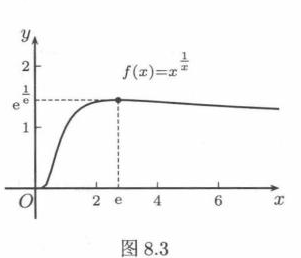
\includegraphics[width=.36\linewidth]{figures/upper/ch08/fig-8-3.png}
\end{center}

由于在一开始时令 $x=a/n$，所以要求 $a/x$ 为正整数。如果 $a/\ee$ 不是正整数，则应当取 $n$ 为多少？

若 $0<a<\ee$，则可以看出 $n=1$，也就是说不分比分好。若 $a/\ee\notin\NN_+$ 且 $a>\ee$，则总可以找到一个正整数 $n$，使得
\[
  \frac{a}{n+1}<\ee<\frac an.
\]
然后比较 $f\left(\frac{a}{n+1}\right)$ 和 $f\left(\frac an\right)$ 的大小，决定将 $a$ 分成 $n$ 份还是 $n+1$ 份。

\begin{xremark}
\textbf{注 1}\quad 另一个与此相关的问题是：若 $a\in\NN_+$，且要求所分成的每一份都是正整数，则应当如何分才能使乘积最大？

这个问题的答案是：首先每一份应当不是 2 就是 3，也就是说与数 $\ee$ 尽可能接近。一旦知道这个结论后，可以用数学归纳法来证明它，并不需要上述微分学的知识。然后，由于 $2+2+2=3+3$，但 $2^3<3^2$，因此在将正整数 $a$ 分成若干个 2 与 3 之和时，2 最多出现两次。这样就将分法完全确定下来，并保证乘积最大。

最后将分法小结如下：设 $a\in\NN_+$。(1) 若 $a$ 是 3 的倍数，则每一份为 3；(2) 若 $a\equiv1\pmod3$，则取两份 2，其余均为 3；(3) 若 $a\equiv2\pmod3$，则取一份 2，其余均为 3。

\textbf{注 2}\quad 在 (8.4) 中的函数的最大值也可以从不等式
\[
  \ee^u\ge1+u
\]
得到，其中仅当 $u=0$ 时成立等号。这从带 Lagrange 余项的 Taylor 公式（其中 $0<\theta<1$）
\[
  \ee^u=1+u+\frac{\ee^{\theta u}}{2!}u^2\ge1+u
\]
就可以得到。然后令
\[
  u=\frac{x-\ee}{\ee}
\]
代入，略加整理，即可得到不等式
\[
  \ee^{1/\ee}\ge x^{1/x},
\]
当且仅当 $x=\ee$ 时成立等号。
\end{xremark}
\end{xsolution}

\begin{xexample}[8.3.4]
问：能通过图 8.4 的直角河道的最长船身是多少？
\end{xexample}
\begin{xsolution}
在图上我们看到宽度为 $a$ 和 $b$ 的河道成直角相接。现在设想将船简化为一个直线段。在图上经过河岸的突出角作出一条斜线段。以图示的角度 $\theta$ 为这个线段位置的参数，$0<\theta<\frac12\pi$。可以看出，能通过直角河道的船身长度在任何情况都不会超出这个线段的长度 $l(\theta)$。由于这对每个 $\theta$ 都成立，因此能通过这个河道的最长船身不会超过
\[
  \min_{0<\theta<\pi/2}\{l(\theta)\}.
\]

\begin{center}
  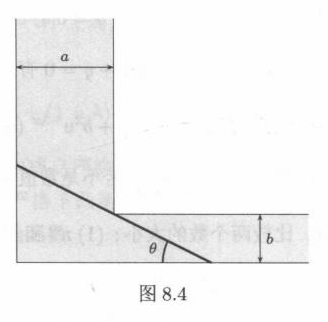
\includegraphics[width=.38\linewidth]{figures/upper/ch08/fig-8-4.png}
\end{center}

另一方面，可以看出，在用一个直线段来表示船时，只要船身不超过这个最小值，船就能够通过这个直角河道。所以求最大船长的问题就转变成为求函数 $l(\theta)$ 的最小值问题，这里自变量 $\theta$ 的范围是 $(0,\pi/2)$。

容易写出函数 $l(\theta)$ 的表达式：
\[
  l(\theta)=a\operatorname{sec}\theta+b\operatorname{csc}\theta,
  \qquad 0<\theta<\frac\pi2.
\]
求导得到
\[
  l'(\theta)=\frac{a\sin\theta}{\cos^2\theta}-\frac{b\cos\theta}{\sin^2\theta}
  =\frac1{\sin^2\theta\cos^2\theta}(a\sin^3\theta-b\cos^3\theta).
\]
由于当 $\theta$ 从 0 变到 $\frac12\pi$ 时最后一个因子 $a\sin^3\theta-b\cos^3\theta$ 的值从 $-b$ 到 $a$ 严格单调增加，因此 $l'(\theta)$ 存在唯一的零点
\[
  \theta_0=\arctan\sqrt[3]{\frac ba}.
\]
从 $l'(\theta)$ 的符号变化可见 $\theta_0$ 是函数 $l(\theta)$ 的最小值点。

最后计算出 $l(\theta)$ 的最小值
\[
  l(\theta_0)=\left(a^{2/3}+b^{2/3}\right)^{3/2},
\]
这就是能通过所示直角河道的最大船身长度。由于我们无法考虑各种船的具体形状，而是将船简化为一个直线段，因此所求出的数值只有参考价值。但是这个值肯定是能通过的船身长度的一个上界。
\end{xsolution}

\subsection{练习题}

\begin{xexercise}[1]
设 $f\in C(I)$，$I$ 为区间，证明：若 $x_0\in I$ 是 $f$ 的唯一极值点，则 $x_0$ 一定是最值点；又若 $x_0$ 是极小值点（极大值点），则它也是 $f$ 的唯一最小值点（唯一最大值点）。
\end{xexercise}
\begin{xsolution}
先设 $x_0$ 是唯一极值点且为极小值点。若它不是全局最小值点，则存在 $y\in I$ 使 $f(y)<f(x_0)$。不妨设 $y>x_0$。由局部极小性，在 $x_0$ 右侧充分小的邻域内 $f(x)\ge f(x_0)$。若该邻域内恒等于 $f(x_0)$，则其中每一点都是极值点，矛盾；故可取 $z\in(x_0,y)$ 使 $f(z)>f(x_0)$。连续函数在 $[x_0,y]$ 上取得最大值，而该最大值既不能在 $x_0$ 取得，也不能在 $y$ 取得，故在内部出现另一个极大值点，矛盾。因此 $x_0$ 是最小值点。极大值情形同理。

若 $x_0$ 是极小值点而另有 $y\ne x_0$ 也取得同一最小值，则在两点之间若函数恒为该值，就有无穷多个极值点；若不恒定，则区间内部有一点取得更大的最大值，从而产生另一个极值点。故 $x_0$ 还是唯一最小值点。极大值情形同理。
\end{xsolution}


\begin{xexercise}[2]
求出方程 $x^3+px+q=0$ 有三个不同实根的充分必要条件。
\end{xexercise}
\begin{xsolution}
设
\[
  F(x)=x^3+px+q.
\]
若有三个不同实根，则必须 $p<0$，否则 $F'(x)=3x^2+p\ge0$，函数单调而不可能有三个不同实根。令
\[
  s=\sqrt{-\frac p3}>0.
\]
此时 $-s$ 为极大值点，$s$ 为极小值点，且
\[
  F(-s)=q+2s^3,\qquad F(s)=q-2s^3.
\]
三条不同实根出现的充分必要条件正是
\[
  F(-s)>0,\qquad F(s)<0,
\]
即
\[
  |q|<2s^3.
\]
化为 $p,q$ 的条件为
\[
  \boxed{\,4p^3+27q^2<0\,},
\]
这本身已包含 $p<0$。
\end{xsolution}


\begin{xexercise}[3]
求出方程 $\dfrac1{x^2}+px+q=0$ 有三个不同实根的充分必要条件。
\end{xexercise}
\begin{xsolution}
令
\[
  F(x)=\frac1{x^2}+px+q,\qquad x\ne0.
\]
若 $p=0$，左右两个半轴上至多各有一个正的 $x^2$ 值，不可能有三个不同实根，故必须 $p\ne0$。

有
\[
  F'(x)=p-\frac2{x^3}.
\]
若 $p>0$，则在 $(-\infty,0)$ 上 $F$ 严格增加，并从 $-\infty$ 变到 $+\infty$，恰有一个负根；在 $(0,+\infty)$ 上只有一个临界点
\[
  x_0=\left(\frac2p\right)^{1/3},
\]
且为极小值点。要在正半轴另有两个不同根，充要条件是
\[
  F(x_0)=q+3\left(\frac p2\right)^{2/3}<0.
\]
$p<0$ 时情形关于原点对称：正半轴恰有一个根，负半轴有两个根的充要条件仍为
\[
  q+3\left(\frac{|p|}{2}\right)^{2/3}<0.
\]
因此总的充分必要条件为
\[
  \boxed{p\ne0,\qquad q<-3\left(\frac{|p|}{2}\right)^{2/3}}.
\]
\end{xsolution}


\begin{xexercise}[4]
证明：$f(x)=a^2\ee^{\lambda x}+b^2\ee^{-\lambda x}$（$a,b>0$）存在与 $\lambda$ 无关的极小值。
\end{xexercise}
\begin{xsolution}
先设 $\lambda\ne0$。由算术平均值－几何平均值不等式，
\[
  a^2\ee^{\lambda x}+b^2\ee^{-\lambda x}
  \ge2ab,
\]
且等号当且仅当
\[
  a^2\ee^{\lambda x}=b^2\ee^{-\lambda x},
  \qquad
  x=\frac1\lambda\ln\frac ba.
\]
故极小值为
\[
  \boxed{2ab},
\]
与 $\lambda$ 无关。

若允许退化参数 $\lambda=0$，则函数恒为 $a^2+b^2$；因此原题“与 $\lambda$ 无关”的通常理解应当排除 $\lambda=0$（或另把这个退化情形列出）。
\end{xsolution}


\begin{xexercise}[5]
证明：$y=\dfrac{ax+b}{cx+d}$ 若不是常值函数，则不会有极值。
\end{xexercise}
\begin{xsolution}
若
\[
  f(x)=\frac{ax+b}{cx+d}
\]
不是常值函数，则 $ad-bc\ne0$。在定义域的每个连通区间上
\[
  f'(x)=\frac{ad-bc}{(cx+d)^2}
\]
恒不为零且符号不变，所以 $f$ 在每个定义区间上严格单调，不存在内点极值。
\end{xsolution}


\begin{xexercise}[6]
比较两个数的大小：(1) $\pi^{\ee}$ 和 $\ee^\pi$；(2) $(\sqrt n)^{\sqrt{n+1}}$ 和 $(\sqrt{n+1})^{\sqrt n}$。
\end{xexercise}
\begin{xsolution}
\begin{enumerate}[label=(\arabic*)]
  \item 比较对数即可。令 $\phi(x)=\ln x/x$。因
  \[
    \phi'(x)=\frac{1-\ln x}{x^2},
  \]
  $\phi$ 在 $[\ee,+\infty)$ 上严格减少。由于 $\pi>\ee$，
  \[
    \frac{\ln\pi}{\pi}<\frac1\ee,
  \]
  即 $\ee\ln\pi<\pi$，故
  \[
    \boxed{\pi^{\ee}<\ee^\pi}.
  \]

  \item 两边取对数并约去正因子 $\sqrt{n(n+1)}/2$，问题等价于比较
  \[
    \psi(n)=\frac{\ln n}{\sqrt n},
    \qquad
    \psi(n+1)=\frac{\ln(n+1)}{\sqrt{n+1}}.
  \]
  有
  \[
    \psi'(x)=\frac{1-\frac12\ln x}{x^{3/2}},
  \]
  故 $\psi$ 在 $(0,\ee^2)$ 上增加，在 $(\ee^2,+\infty)$ 上减少。于是 $1\le n\le6$ 时
  \[
    (\sqrt n)^{\sqrt{n+1}}<(\sqrt{n+1})^{\sqrt n};
  \]
  $n\ge8$ 时不等号反向。对唯一跨过极大点的整数 $n=7$ 直接比较
  \[
    \frac{\ln7}{\sqrt7}>\frac{\ln8}{\sqrt8}
  \]
  （两边数值约为 $0.73545$ 与 $0.73519$），所以 $n=7$ 时也为反向不等号。综上，$n\le6$ 时右边较大，$n\ge7$ 时左边较大。
\end{enumerate}
\end{xsolution}


\begin{xexercise}[7]
考虑下列几何极值问题（能用初等方法做就不一定用微分学工具）：
  \begin{enumerate}[label=(\arabic*)]
    \item 在面积为定值的三角形中，什么三角形的周长最小？
    \item 在周长为定值的三角形中，什么三角形的面积最大？
    \item 在椭圆 $\dfrac{x^2}{a^2}+\dfrac{y^2}{b^2}=1$ 内，各边平行于坐标轴的内接矩形中，面积最大的矩形的长和宽分别为多少？
    \item 在椭圆 $\dfrac{x^2}{a^2}+\dfrac{y^2}{b^2}=1$ 内，各边平行于坐标轴的内接矩形中，周长最大的矩形的长和宽为多少？
  \end{enumerate}
\end{xexercise}
\begin{xsolution}
\begin{enumerate}[label=(\arabic*)]
  \item 设三角形面积为 $K$，半周长为 $s$。令
  \[
    x=s-a,\quad y=s-b,\quad z=s-c,
  \]
  则 $x+y+z=s$，Heron 公式给出 $K^2=sxyz$。由
  \[
    xyz\le\left(\frac s3\right)^3
  \]
  得
  \[
    K^2\le\frac{s^4}{27}.
  \]
  固定 $K$ 时，$s$ 因而有确定的下界，且等号当且仅当 $x=y=z$，即 $a=b=c$。故周长最小的是等边三角形。

  \item 固定周长即固定 $s$。同一公式
  \[
    K^2=sxyz\le s\left(\frac s3\right)^3
  \]
  表明面积最大当且仅当 $x=y=z$，故仍为等边三角形。

  \item 取第一象限顶点 $(x,y)$，矩形的长、宽为 $2x,2y$，且
  \[
    \frac{x^2}{a^2}+\frac{y^2}{b^2}=1.
  \]
  令 $u=x/a$，$v=y/b$，则 $u^2+v^2=1$。面积
  \[
    4xy=4abuv\le2ab,
  \]
  等号在 $u=v=1/\sqrt2$ 时成立。因此最大面积矩形的长、宽为
  \[
    \boxed{\sqrt2\,a,\qquad \sqrt2\,b}.
  \]

  \item 周长为 $4(x+y)$。由 Cauchy 不等式
  \[
    x+y=au+bv\le\sqrt{a^2+b^2}\sqrt{u^2+v^2}=\sqrt{a^2+b^2},
  \]
  等号在
  \[
    u=\frac a{\sqrt{a^2+b^2}},\qquad
    v=\frac b{\sqrt{a^2+b^2}}
  \]
  时成立。因此所求长、宽为
  \[
    \boxed{
    \frac{2a^2}{\sqrt{a^2+b^2}},\qquad
    \frac{2b^2}{\sqrt{a^2+b^2}}}.
  \]
\end{enumerate}
\end{xsolution}


\begin{xexercise}[8]
考虑给定边界值的二阶线性非齐次微分方程
  \[
    y''+p(x)y'+q(x)y=r(x),\quad a<x<b,\quad y(a)=A,\quad y(b)=B,
  \]
  其中 $p,q,r$ 是给定的函数，$A$ 和 $B$ 是给定的数。又设 $q(x)<0$，$\forall x\in(a,b)$，证明：如果这个微分方程在闭区间 $[a,b]$ 上存在解，则必唯一。
\end{xexercise}
\begin{xsolution}
设 $y_1,y_2$ 是两个满足同一边界条件的解，令 $z=y_1-y_2$，则
\[
  z''+p(x)z'+q(x)z=0,
  \qquad z(a)=z(b)=0.
\]
若 $z\not\equiv0$，则连续函数 $z$ 在 $(a,b)$ 内或者取得正的最大值，或者取得负的最小值。

若在 $x_0$ 处取得正最大值，则 $z'(x_0)=0$、$z''(x_0)\le0$，但微分方程给出
\[
  z''(x_0)=-q(x_0)z(x_0)>0,
\]
矛盾。若取得负最小值，则 $z'(x_0)=0$、$z''(x_0)\ge0$，而
\[
  z''(x_0)=-q(x_0)z(x_0)<0,
\]
也矛盾。故 $z\equiv0$，解唯一。
\end{xsolution}


\begin{xremark}
前面与极值问题有关的材料还有 5.3.3 小节的题 9，第五章第二组参考题 16--18。
\end{xremark}

\section{函数的凸性}

凸函数是有广泛应用的一类重要函数。它与凸集的研究一起已形成为一个专门的方向——凸分析。有关凸函数的试题经常在考研试卷中出现，有时在高考试卷中也会出现。本节将介绍凸函数的基本事实。关于用凸函数为工具来证明不等式则将在下一节的 8.5.2 小节内介绍。与积分有关的凸函数性质见第十一章的 11.2.1 小节的凸函数不等式和部分参考题。

\subsection{基本命题}

\begin{xdefinition}
设函数 $f$ 在区间 $I$ 上定义。若对每一对点 $x_1,x_2\in I$，$x_1\ne x_2$ 和每个 $\lambda\in(0,1)$，成立不等式
\begin{equation}
  f(\lambda x_1+(1-\lambda)x_2)\le\lambda f(x_1)+(1-\lambda)f(x_2),
  \tag{8.5}
  \label{eq:8.5}
\end{equation}
则称 $f$ 为区间 $I$ 上的\textbf{下凸函数}。又若在 (8.5) 中成立严格不等号，则称 $f$ 为区间 $I$ 上的\textbf{严格下凸函数}。若函数 $-f$ 为下凸函数（严格下凸函数），则称 $f$ 为\textbf{上凸函数}（严格上凸函数）。下凸函数和上凸函数统称为凸函数。
\end{xdefinition}

\begin{xremark}
请读者注意：下凸函数和上凸函数的名称在我国的数学分析教学中使用已久，它们与向下凸和向上凸的直观说法一致，方便易记；但也有很多教科书和其他文献使用凸函数和凹函数的名称，因为下凸函数和上凸函数在英语中分别为 convex function 和 concave function。
\end{xremark}

凸函数的定义有明显的几何意义。在图 8.5 中我们看到下凸条件 (8.5) 表明，连接该函数图像 $y=f(x)$ 上的任意两点的直线段应当在相应的曲线段的上方。在下一个命题中我们将对条件 (8.5) 作进一步的发掘，从而得到更多的等价条件，这在研究凸函数时非常有用。

\begin{xtheorem}[8.4.1]
函数 $f$ 在区间 $I$ 上为下凸的充分必要条件是对于区间 $I$ 中的任意三点 $x_1<x_2<x_3$，成立不等式
\begin{equation}
  \frac{f(x_2)-f(x_1)}{x_2-x_1}
  \le\frac{f(x_3)-f(x_1)}{x_3-x_1}
  \le\frac{f(x_3)-f(x_2)}{x_3-x_2}.
  \tag{8.6}
  \label{eq:8.6}
\end{equation}
又如在不等式中的不等号“$\le$”都改为严格的不等号“$<$”，则就是严格下凸的充分必要条件。
\end{xtheorem}

\paragraph{分析}
在证明之前先分析条件 (8.6) 的意义。

\begin{center}
  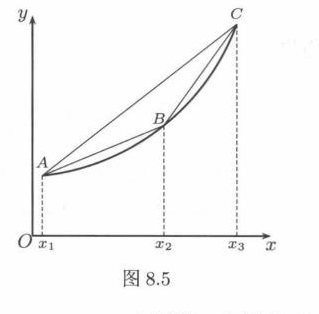
\includegraphics[width=.42\linewidth]{figures/upper/ch08/fig-8-5.png}
\end{center}

如图 8.5 所示，将坐标平面上的三个点 $(x_1,f(x_1))$，$(x_2,f(x_2))$，$(x_3,f(x_3))$ 记为点 $A,B,C$，又用 $k(\overline{AB})$，$k(\overline{BC})$，$k(\overline{AC})$ 表示直线段 $AB,BC,AC$ 的斜率，则可以将条件 (8.6) 改写为
\begin{equation}
  k(\overline{AB})\le k(\overline{AC})\le k(\overline{BC}).
  \tag{8.7}
  \label{eq:8.7}
\end{equation}
但这个条件实际上含有三个不等式：
\begin{equation}
  k(\overline{AB})\le k(\overline{AC}),\qquad
  k(\overline{AB})\le k(\overline{BC}),\qquad
  k(\overline{AC})\le k(\overline{BC}).
  \tag{8.8}
  \label{eq:8.8}
\end{equation}
利用行列式计算容易得到下列等式：
\begin{align*}
\begin{vmatrix}
1&1&1\\
x_1&x_2&x_3\\
f(x_1)&f(x_2)&f(x_3)
\end{vmatrix}
&=
\begin{vmatrix}
x_2-x_1&x_3-x_1\\
f(x_2)-f(x_1)&f(x_3)-f(x_1)
\end{vmatrix}\\
&=
\begin{vmatrix}
x_2-x_1&x_3-x_2\\
f(x_2)-f(x_1)&f(x_3)-f(x_2)
\end{vmatrix}\\
&=
\begin{vmatrix}
x_3-x_1&x_3-x_2\\
f(x_3)-f(x_1)&f(x_3)-f(x_2)
\end{vmatrix}.
\end{align*}
由于三个二阶行列式非负的条件恰好分别对应了 (8.8) 中的三个不等式，因此这三个不等式相互等价。\footnote{用向量代数中的外积和混合积可对以上四个行列式非负的条件给出几何解释，这里从略。}这样在下面命题 8.4.1 的证明中只需要证明下凸函数的定义和这三个不等式中的某一个等价即可。

\paragraph{命题 8.4.1 的证明}
（只写出下凸函数的证明，关于严格下凸函数的证明从略。）由给定的 $x_1<x_2<x_3$ 可以计算出
\[
  \lambda=\frac{x_3-x_2}{x_3-x_1},
\]
它满足条件 $0<\lambda<1$ 和等式
\[
  x_2=\lambda x_1+(1-\lambda)x_3.
\]
先证必要性。由于 $f$ 下凸，有
\[
  f(x_2)\le\lambda f(x_1)+(1-\lambda)f(x_3).
\]
将 $\lambda$ 的表达式代入，再加整理，就得到
\[
  (x_3-x_1)[f(x_2)-f(x_1)]\le(x_2-x_1)[f(x_3)-f(x_1)],
\]
这就是 $k(\overline{AB})\le k(\overline{AC})$。

再证充分性。任取一个不等式，例如 $k(\overline{AB})\le k(\overline{AC})$，就可以改写为
\[
  f(\lambda x_1+(1-\lambda)x_3)\le\lambda f(x_1)+(1-\lambda)f(x_3).
\]
由于 $x_1<x_2<x_3$，同时它们又是区间 $I$ 中的任意三点，因此就证明了 $f$ 在 $I$ 上为下凸函数。

\begin{xtheorem}[8.4.2]
开区间上的凸函数必是连续函数。
\end{xtheorem}
\paragraph{分析}
先作几何观察。不妨只讨论下凸函数。设 $f$ 为开区间 $I$ 上的下凸函数，点 $x_0\in I$。如图 8.6 所示，在开区间 $I$ 中于 $x_0$ 两侧取 $x_1<x_0<x_2$，记坐标平面上的点 $(x_1,f(x_1))$，$(x_0,f(x_0))$，$(x_2,f(x_2))$ 为 $A,B,C$。先从几何上分析如何可以证明 $f$ 于点 $x_0$ 右连续。

取 $x_0<x<x_2$，并在图 8.6 上标出三个点 $a,b,c$，它们分别是在坐标平面上过点 $(x,0)$ 而平行于 $y$ 轴的直线与直线段 $BC$、曲线 $y=f(x)$ 和直线段 $AB$ 的延长线的交点。容易看出，在 $x\to x_0+$ 时，点 $a$ 和 $c$ 沿直线趋于点 $B$，若能证明点 $b$ 确实在 $a,c$ 之间，则证明就完成了。以下即是将这些几何上的观察翻译成分析语言。

\begin{center}
  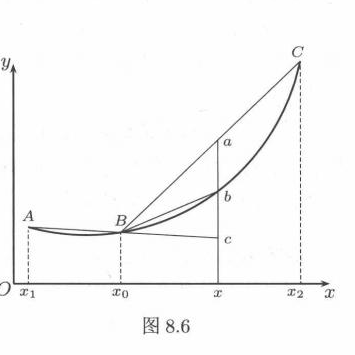
\includegraphics[width=.43\linewidth]{figures/upper/ch08/fig-8-6.png}
\end{center}

\begin{xproof}
对 $x_1<x_0<x$ 和 $x_0<x<x_2$ 分别应用命题 8.4.1，就得到
\begin{equation}
  k(\overline{BC})\le k(\overline{Bb})\le k(\overline{Ba}).
  \tag{8.9}
  \label{eq:8.9}
\end{equation}
由于 $x_0<x$，不等式 (8.9) 等价于在 $a,b,c$ 三点的纵坐标之间的下列序关系：
\[
  \frac{x-x_0}{x_0-x_1}[f(x_0)-f(x_1)]+f(x_0)
  \le f(x)
  \le\frac{x_2-x}{x_2-x_0}f(x_0)+\frac{x-x_0}{x_2-x_0}f(x_2).
\]
令 $x\to x_0+$，用夹逼定理，就得到
\[
  \lim_{x\to x_0+}f(x)=f(x_0).
\]
关于 $f$ 在点 $x_0$ 为左连续的证明完全类似，从略。
\end{xproof}

\begin{xremark}
若凸函数的定义域不是开区间，则在端点处可以不连续。例如，
\[
  f(x)=
  \begin{cases}
    1,&x=0,1,\\
    0,&0<x<1
  \end{cases}
\]
在闭区间 $[0,1]$ 上是下凸函数，但在端点处不连续。
\end{xremark}

\begin{xtheorem}[8.4.3]
若 $f$ 为开区间 $I$ 上的下凸函数，则

(1) $f$ 处处存在有限的两个单侧导数，而且成立不等式 $f'_-(x)\le f'_+(x)$，$x\in I$；

(2) 对任何 $x,y\in I$，$x<y$，成立不等式
\[
  f'_-(x)\le f'_+(x)\le f'_-(y)\le f'_+(y),
\]
由此知道 $f'_-$ 和 $f'_+$ 均为单调增加函数。
\end{xtheorem}
\begin{xproof}
只要利用不等式 (8.6) 和图 8.5、8.6 就够了。

(1) 利用 (8.8) 中的第二个不等式，在图 8.6 上有 $k(\overline{Bb})\le k(\overline{BC})$，而且可以看出当 $x\to x_0+$ 时，$k(\overline{Bb})$ 单调减少，同时又以 $k(\overline{Bc})$ 为下界，因此一定有极限。这就证明了 $f'_+(x_0)$ 存在。类似地可以证明 $f'_-(x_0)$ 的存在性。

(2) 观察图 8.5，利用 (8.6)，再分别令 $x_2\to x_1+$ 和 $x_2\to x_3-$，由于在 (1) 中已经证明了两个单侧导数的存在性，因此就得到 $f'_+(x_1)\le k(\overline{AC})\le f'_-(x_3)$。将 $x_1,x_3$ 改记为 $x,y$ 即可。
\end{xproof}

\begin{xremark}
由于命题 8.4.3 的证明不需要用命题 8.4.2 的结论，因此很多文献中将后者作为前者的推论得到，即从两个单侧导数存在推出连续。从命题 8.4.2 的证明可见，直接证明连续性也是容易的。
\end{xremark}

\begin{xtheorem}[8.4.4]
设 $f$ 在区间 $I$ 上可微，则

(1) $f$ 在 $I$ 上为下凸函数的充分必要条件是 $f'$ 在 $I$ 上为单调增加函数；

(2) $f$ 在 $I$ 上为严格下凸函数的充分必要条件是 $f'$ 在 $I$ 上严格单调增加。
\end{xtheorem}
\begin{xproof}
先给出 (1) 的充分性部分的证明。利用命题 8.4.1 和对其结果（在证明前）的分析，可见只需要证明对曲线 $y=f(x)$ 上自左到右的任意不同三点 $A,B,C$ 成立
\[
  k(\overline{AB})\le k(\overline{BC}).
\]
设 $f'$ 在区间 $I$ 上单调增加。取 $x_1,x_2\in I$，$x_1<x_2$，$\lambda\in(0,1)$。引入
\[
  x_\lambda=\lambda x_1+(1-\lambda)x_2.
\]
将点 $(x_1,f(x_1))$，$(x_\lambda,f(x_\lambda))$，$(x_2,f(x_2))$ 分别记为 $A,B,C$，则就有
\[
  k(\overline{AB})=\frac{f(x_\lambda)-f(x_1)}{x_\lambda-x_1},
  \qquad
  k(\overline{BC})=\frac{f(x_2)-f(x_\lambda)}{x_2-x_\lambda}.
\]
对右边的两个差商用 Lagrange 微分中值定理，分别得到 $f'(\xi_1)$ 和 $f'(\xi_2)$，其中
\[
  \xi_1\in(x_1,x_\lambda),\qquad \xi_2\in(x_\lambda,x_2).
\]
由于 $\xi_1<\xi_2$，利用条件 $f'$ 为单调增加，因此有
\begin{equation}
  f'(\xi_1)\le f'(\xi_2).
  \tag{8.10}
  \label{eq:8.10}
\end{equation}
这样就得到所要的结果
\[
  k(\overline{AB})\le k(\overline{BC}).
\]

(1) 的必要性部分可由命题 8.4.3 之 (2) 得出。

关于 (2) 的证明只概述如下：充分性部分可从上面看出。由于 $f'$ 严格单调增加，因此从 $\xi_1<\xi_2$ 可见不等式 (8.10) 成立严格不等号，即有 $k(\overline{AB})<k(\overline{BC})$。由命题 8.4.1 的证明过程可知这时就保证了 $f$ 严格下凸。

又若 $f'$ 单调增加但不是严格单调增加，则在区间 $I$ 上存在点 $x_1<x_2$，使得 $f'(x)$ 在子区间 $[x_1,x_2]$ 上为常值函数，从而 $f$ 在区间 $[x_1,x_2]$ 上是线性函数，而不可能是严格下凸函数。这样就完成了必要性的证明。
\end{xproof}

\begin{xtheorem}[8.4.5]
若 $f$ 是区间 $I$ 上的可微下凸函数，则经过点 $(x_0,f(x_0))$（$x_0\in I$）的切线一定在曲线 $y=f(x)$ 的下方，即成立不等式
\[
  f(x)\ge f(x_0)+f'(x_0)(x-x_0),\qquad\forall x\in I.
\]
又若 $f$ 严格下凸，则上述不等式成立等号的充分必要条件是 $x=x_0$。
\end{xtheorem}
\begin{xproof}
将上述不等式的右边移项到左边，然后用 Lagrange 中值定理，就有
\[
  f(x)-f(x_0)-f'(x_0)(x-x_0)=(f'(\xi)-f'(x_0))(x-x_0),
\]
其中 $\xi\in(x_0,x)$ 或 $(x,x_0)$。用命题 8.4.4 可见上式非负，而在 $f$ 为严格下凸时，$f'$ 为严格单调，因此仅当 $x=x_0$ 时为 0。
\end{xproof}

\begin{xremark}
称直线 $y=f(x_0)+f'(x_0)(x-x_0)$ 为凸函数 $f$ 在点 $(x_0,f(x_0))$ 处的\textbf{支撑线}。若去掉可微条件，则仍存在相应的支撑线，见 8.4.2 小节的题 11。
\end{xremark}

\begin{xtheorem}[8.4.6]
设函数 $f$ 于区间 $I$ 上二阶可微，则

(1) $f$ 在 $I$ 上为下凸函数的充分必要条件是在 $I$ 上处处有 $f''(x)\ge0$；

(2) $f$ 在 $I$ 上为严格下凸函数的充分必要条件是在 $I$ 上处处有 $f''(x)\ge0$，而且在任一正长度的子区间上 $f''(x)$ 不恒等于零。
\end{xtheorem}

这个命题可以从命题 8.4.4 的结论直接得出，但也可以证明如下。

\begin{xproof}
（只证明 (1)）先证必要性。对区间的内点 $x$，取 $h>0$ 充分小，就可以由下凸性推出不等式
\[
  f(x)\le\frac12[f(x-h)+f(x+h)].
\]
这保证了下列极限非负：
\[
  \lim_{h\to0}\frac{f(x+h)-2f(x)+f(x-h)}{h^2}=f''(x).
\]
对端点可由 Darboux 定理推出。

再证充分性。如命题 8.4.4 证明一开始那样对 $x_1<x_2$ 和 $0<\lambda<1$ 引入 $x_\lambda$，并写出 $f(x_1)$ 和 $f(x_2)$ 在点 $x_\lambda$ 的带 Lagrange 型余项的 Taylor 公式：
\[
  f(x_1)=f(x_\lambda)+f'(x_\lambda)(x_1-x_\lambda)+\frac12f''(\xi_1)(x_1-x_\lambda)^2,
\]
\[
  f(x_2)=f(x_\lambda)+f'(x_\lambda)(x_2-x_\lambda)+\frac12f''(\xi_2)(x_2-x_\lambda)^2,
\]
其中 $\xi_1\in(x_1,x_\lambda)$，$\xi_2\in(x_\lambda,x_2)$。将第一式乘 $\lambda$ 与第二式乘 $(1-\lambda)$ 相加，利用二阶导数非负和 $x_\lambda=\lambda x_1+(1-\lambda)x_2$，就得到所要的不等式
\[
  \lambda f(x_1)+(1-\lambda)f(x_2)\ge f(x_\lambda).
\]
\end{xproof}

\begin{xtheorem}[8.4.7（下凸函数的 Jensen（詹森）不等式）]
如 $f$ 为区间 $I$ 上的二阶可微下凸函数，则对任何 $x_1,x_2,\ldots,x_n\in I$ 与满足条件 $\lambda_1+\lambda_2+\cdots+\lambda_n=1$ 的 $n$ 个正数 $\lambda_1,\lambda_2,\ldots,\lambda_n$ 成立不等式
\begin{equation}
  \lambda_1f(x_1)+\lambda_2f(x_2)+\cdots+\lambda_nf(x_n)
  \ge f(\lambda_1x_1+\lambda_2x_2+\cdots+\lambda_nx_n).
  \tag{8.11}
  \label{eq:8.11}
\end{equation}
又若 $f$ 严格下凸，则上述不等式成立等号的充分必要条件是
\begin{equation}
  x_1=x_2=\cdots=x_n.
  \tag{8.12}
  \label{eq:8.12}
\end{equation}
\end{xtheorem}
\begin{xproof}
记 $\bar x=\lambda_1x_1+\lambda_2x_2+\cdots+\lambda_nx_n$（即数 $x_1,x_2,\ldots,x_n$ 的加权平均值），并写出 $f(x_i)$（$i=1,2,\ldots,n$）在点 $\bar x$ 的带 Lagrange 余项的 Taylor 公式：
\[
  f(x_i)=f(\bar x)+f'(\bar x)(x_i-\bar x)+\frac{f''(\xi_i)}{2!}(x_i-\bar x)^2,
  \quad i=1,2,\ldots,n.
\]
将这 $n$ 个公式分别乘以 $\lambda_1,\lambda_2,\ldots,\lambda_n$ 后相加，利用条件 $\lambda_1+\lambda_2+\cdots+\lambda_n=1$ 和二阶导数非负，就得到 Jensen 不等式：
\[
  \lambda_1f(x_1)+\lambda_2f(x_2)+\cdots+\lambda_nf(x_n)
  \ge f(\bar x)+f'(\bar x)(\bar x-\bar x)=f(\bar x).
\]
以下讨论当 $f$ 严格下凸时，在 Jensen 不等式中成立等号的条件。

若在上述不等式中成立等号，则由于每个 $\lambda_i>0$（$i=1,2,\ldots,n$），从以上证明过程可以看出只能是对每个 $i=1,2,\ldots,n$ 成立
\[
  f(x_i)=f(\bar x)+f'(\bar x)(x_i-\bar x).
\]
用命题 8.4.5，可见只能有 $x_i=\bar x$。

反之是明显的。若条件 (8.12) 成立，则对每个 $i=1,2,\ldots,n$ 有 $x_i=\bar x$，因此在上面的不等式中成立等号。
\end{xproof}

\begin{xremark}
命题中的二阶可微条件并非必要（作为下面的练习题 1）。但从应用来看，用二阶导数来检验凸性较为方便。这在 8.5.2 小节中有很多例题可供参考。
\end{xremark}

以下是一个与凸性密切相关的概念，它在许多方面有应用。

\begin{xdefinition}
称曲线 $y=f(x)$ 上的点 $(x_0,f(x_0))$ 为\textbf{拐点}（或\textbf{变曲点}），如果在该点两侧邻近的曲线具有不同的严格凸性。
\end{xdefinition}

关于拐点的基本命题见下面练习题的最后几个题。

\subsection{练习题}

\begin{xexercise}[1]
在不假定函数 $f$ 可微的条件下，证明 Jensen 不等式 (8.11) 仍然成立。
\end{xexercise}
\begin{xsolution}
对 $n$ 作归纳。$n=2$ 时就是下凸函数的定义。设结论对 $n-1$ 个点成立。令
\[
  \mu=\lambda_1+\cdots+\lambda_{n-1}=1-\lambda_n,
  \qquad
  y=\frac1\mu\sum_{i=1}^{n-1}\lambda_i x_i.
\]
由两点下凸性及归纳假设，
\begin{align*}
  f\left(\sum_{i=1}^n\lambda_i x_i\right)
  &=f(\mu y+\lambda_nx_n)\\
  &\le \mu f(y)+\lambda_nf(x_n)\\
  &\le \sum_{i=1}^{n-1}\lambda_i f(x_i)+\lambda_nf(x_n).
\end{align*}
故 Jensen 不等式对任意下凸函数成立，不需可微条件。
\end{xsolution}


\begin{xexercise}[2]
设 $f$ 是区间 $(a,b)$ 上的上凸函数，且 $f(x)>0$，证明：函数 $1/f$ 是区间 $(a,b)$ 上的下凸函数。又问：若在上题中将 $f$ 的上凸条件改为下凸，则有何结论？

  （本题的变形是对 $f$ 加上一阶可微或二阶可微条件。）
\end{xexercise}
\begin{xsolution}
设 $z=\lambda x+(1-\lambda)y$，$0<\lambda<1$。因 $f$ 上凸且为正，
\[
  f(z)\ge \lambda f(x)+(1-\lambda)f(y)>0.
\]
取倒数并利用 $u\mapsto1/u$ 在 $(0,+\infty)$ 上下凸，得到
\begin{align*}
  \frac1{f(z)}
  &\le\frac1{\lambda f(x)+(1-\lambda)f(y)}\\
  &\le\frac\lambda{f(x)}+\frac{1-\lambda}{f(y)}.
\end{align*}
故 $1/f$ 下凸。

若把 $f$ 的条件改成下凸，则一般没有确定结论。例如 $f(x)=1+x^2$ 在 $\RR$ 上正且下凸，而
\[
  \left(\frac1{1+x^2}\right)''
  =\frac{2(3x^2-1)}{(1+x^2)^3}
\]
变号，所以 $1/f$ 既非全局下凸也非全局上凸。
\end{xsolution}


\begin{xexercise}[3]
设 $f,g$ 是 $(a,b)$ 上的下凸函数，证明：$\max\{f,g\}$ 也是 $(a,b)$ 上的下凸函数。
\end{xexercise}
\begin{xsolution}
令 $h=\max\{f,g\}$。对 $z=\lambda x+(1-\lambda)y$，有
\begin{align*}
  h(z)
  &=\max\{f(z),g(z)\}\\
  &\le\max\{\lambda f(x)+(1-\lambda)f(y),
             \lambda g(x)+(1-\lambda)g(y)\}\\
  &\le\lambda h(x)+(1-\lambda)h(y).
\end{align*}
故 $h$ 下凸。
\end{xsolution}


\begin{xexercise}[4]
设 $f$ 和 $g$ 均为区间 $I$ 上的单调增加非负下凸函数，证明：$f\cdot g$ 为区间 $I$ 上的下凸函数。
\end{xexercise}
\begin{xsolution}
设 $x<y$，$z=\lambda x+(1-\lambda)y$。记
\[
  a=f(x),\ b=f(y),\ c=g(x),\ d=g(y).
\]
由单调增加及非负性，$0\le a\le b$，$0\le c\le d$。由下凸性，
\[
  f(z)g(z)\le[\lambda a+(1-\lambda)b][\lambda c+(1-\lambda)d].
\]
而
\begin{align*}
 &\lambda ac+(1-\lambda)bd
 -[\lambda a+(1-\lambda)b][\lambda c+(1-\lambda)d]\\
 &=\lambda(1-\lambda)(b-a)(d-c)\ge0.
\end{align*}
故
\[
  f(z)g(z)\le\lambda f(x)g(x)+(1-\lambda)f(y)g(y),
\]
即 $fg$ 下凸。
\end{xsolution}


\begin{xexercise}[5]
设 $f$ 在区间 $I$ 上为下凸函数，证明：$F(x)=\ee^{f(x)}$ 也是 $I$ 上的下凸函数。
\end{xexercise}
\begin{xsolution}
设 $z=\lambda x+(1-\lambda)y$。由 $f$ 下凸且指数函数严格增加，
\[
  \ee^{f(z)}\le \ee^{\lambda f(x)+(1-\lambda)f(y)}.
\]
又因 $u\mapsto\ee^u$ 下凸，
\[
  \ee^{\lambda f(x)+(1-\lambda)f(y)}
  \le\lambda\ee^{f(x)}+(1-\lambda)\ee^{f(y)}.
\]
故 $F(x)=\ee^{f(x)}$ 下凸。
\end{xsolution}


\begin{xexercise}[6]
设 $f$ 和 $g$ 为 $(-\infty,+\infty)$ 上的下凸函数，问：复合函数 $f\circ g$ 是否一定是 $(-\infty,+\infty)$ 上的下凸函数？
\end{xexercise}
\begin{xsolution}
不一定。例如
\[
  f(u)=\ee^{-u},\qquad g(x)=x^2
\]
都是 $\RR$ 上的下凸函数，但
\[
  (f\circ g)(x)=\ee^{-x^2},
  \qquad
  (f\circ g)''(x)=(4x^2-2)\ee^{-x^2},
\]
二阶导数在 $x=0$ 附近为负，所以复合函数并非下凸函数。
\end{xsolution}


\begin{xexercise}[7]
设 $f$ 为 $(-\infty,+\infty)$ 上的下凸函数，证明：或者 $f$ 为单调函数，或者存在点 $c$，使得 $f$ 在 $(-\infty,c]$ 上单调减少，而在 $[c,+\infty)$ 上单调增加。
\end{xexercise}
\begin{xsolution}
由下凸函数的单侧导数性质，$f'_-$ 与 $f'_+$ 均单调增加。若所有单侧斜率均非负，则 $f$ 单调增加；若均非正，则 $f$ 单调减少。

余下情形中，负斜率与正斜率都出现。令
\[
  c=\sup\{x\in\RR\mid f'_+(x)<0\}.
\]
单侧导数的单调性表明：在 $x<c$ 的范围内各割线斜率非正，而在 $x>c$ 的范围内各割线斜率非负。由命题 8.4.1 的割线斜率刻画可得 $f$ 在 $(-\infty,c]$ 上单调减少，在 $[c,+\infty)$ 上单调增加。端点处若存在一段斜率为零，只需把 $c$ 取在该常值区间内即可。
\end{xsolution}


\begin{xexercise}[8]
设 $f$ 在 $(-\infty,+\infty)$ 上有界，且处处有 $f''(x)\ge0$，证明：$f$ 只能是常值函数。
\end{xexercise}
\begin{xsolution}
由 $f''\ge0$，函数 $f$ 下凸，故任一点的切线都是支撑线。若某点 $x_0$ 有 $f'(x_0)>0$，则
\[
  f(x)\ge f(x_0)+f'(x_0)(x-x_0)\to+\infty
  \quad(x\to+\infty),
\]
与有界矛盾。若 $f'(x_0)<0$，令 $x\to-\infty$ 同样矛盾。因此 $f'(x)=0$ 对一切 $x$ 成立，故 $f$ 为常值函数。
\end{xsolution}


\begin{xexercise}[9]
设 $f$ 在 $(a,b)$ 上 $n$ 阶可微（$n>2$），$f^{(n)}(x)>0$。又有 $x_0\in(a,b)$，使对于 $k=1,2,\ldots,n-1$ 成立 $f^{(k)}(x_0)=0$，证明：
  \begin{enumerate}[label=(\arabic*)]
    \item $n$ 为奇数时，$f$ 在 $(a,b)$ 上严格单调增加；
    \item $n$ 为偶数时，$f$ 在 $(a,b)$ 上严格下凸。
  \end{enumerate}
\end{xexercise}
\begin{xsolution}
因为 $f^{(n)}(x)>0$，由导数的 Darboux 性质及中值定理，$f^{(n-1)}$ 严格增加，而 $f^{(n-1)}(x_0)=0$，所以它在 $x_0$ 左负右正。逐级积分（或反复用中值定理）可知：每下降一次求导阶数，符号在左侧交替一次、右侧保持为正。

当 $n$ 为奇数时，从 $f^{(n)}$ 下降到 $f'$ 共 $n-1$ 次，$n-1$ 为偶数，因此 $f'(x)>0$ 对 $x\ne x_0$ 成立，而 $f'(x_0)=0$，故 $f$ 在 $(a,b)$ 上严格单调增加。

当 $n$ 为偶数时，从 $f^{(n)}$ 下降到 $f''$ 共 $n-2$ 次，$n-2$ 为偶数，因此 $f''(x)>0$ 对 $x\ne x_0$ 成立，而 $f''(x_0)=0$。故 $f'$ 严格单调增加，从而 $f$ 在 $(a,b)$ 上严格下凸。
\end{xsolution}


\begin{xexercise}[10]
设 $f$ 在开区间 $(c,d)$ 上为下凸函数，则 $f$ 一定满足内闭的 Lipschitz 条件。（这就是说对每个有界闭区间 $[a,b]\subset(c,d)$，存在 $M>0$，对所有 $x_1,x_2\in[a,b]$，成立 $|f(x_1)-f(x_2)|\le M|x_1-x_2|$。）
\end{xexercise}
\begin{xsolution}
任取闭区间 $[a,b]\subset(c,d)$。再取 $\alpha,\beta$ 使
\[
  c<\alpha<a<b<\beta<d.
\]
对任意 $a\le x_1<x_2\le b$，由下凸函数三点斜率不等式，
\[
  \frac{f(a)-f(\alpha)}{a-\alpha}
  \le\frac{f(x_2)-f(x_1)}{x_2-x_1}
  \le\frac{f(\beta)-f(b)}{\beta-b}.
\]
令两端常数分别为 $m,M$，则
\[
  \left|\frac{f(x_2)-f(x_1)}{x_2-x_1}\right|
  \le\max\{|m|,|M|\}.
\]
故 $f$ 在 $[a,b]$ 上满足 Lipschitz 条件。
\end{xsolution}


\begin{xexercise}[11]
证明：$f$ 在开区间 $I$ 上为下凸函数的充分必要条件是对每个 $c\in I$，存在 $a$，使在区间 $I$ 上成立不等式 $f(x)\ge a(x-c)+f(c)$（称 $y=a(x-c)+f(c)$ 为支撑线）。
\end{xexercise}
\begin{xsolution}
先设 $f$ 下凸。固定 $c\in I$。由命题 8.4.3，有限单侧导数满足
\[
  f'_-(c)\le f'_+(c).
\]
任取
\[
  a\in[f'_-(c),f'_+(c)].
\]
若 $x<c$，割线斜率不大于 $f'_-(c)\le a$；若 $x>c$，割线斜率不小于 $f'_+(c)\ge a$。两种情形都给出
\[
  f(x)\ge f(c)+a(x-c).
\]

反之，设每个 $c$ 都存在这样的支撑线。对任意 $x_1<x_2<x_3$，在 $c=x_2$ 取支撑线斜率 $a$，则
\[
  \frac{f(x_2)-f(x_1)}{x_2-x_1}\le a
  \le\frac{f(x_3)-f(x_2)}{x_3-x_2}.
\]
由命题 8.4.1，$f$ 下凸。
\end{xsolution}


\begin{xexercise}[12]
设 $f$ 在 $[a,+\infty)$ 上为凸函数，证明：$\displaystyle\lim_{x\to+\infty}\frac{f(x)}x$ 一定有意义。
\end{xexercise}
\begin{xsolution}
对 $x>a$ 定义
\[
  q(x)=\frac{f(x)-f(a)}{x-a}.
\]
由凸函数三点斜率不等式，$q(x)$ 单调增加，故
\[
  L=\lim_{x\to+\infty}q(x)
\]
在扩充实数意义下存在（可能为 $+\infty$）。又
\[
  \frac{f(x)}x=\frac{x-a}{x}q(x)+\frac{f(a)}x,
\]
所以
\[
  \lim_{x\to+\infty}\frac{f(x)}x=L.
\]
这说明该极限一定有意义。
\end{xsolution}


\begin{xexercise}[13]
设 $f$ 在 $(-\infty,+\infty)$ 上为凸函数，又有 $\displaystyle\lim_{x\to\pm\infty}\frac{f(x)}x=0$，证明：$f$ 是常值函数。
\end{xexercise}
\begin{xsolution}
若 $f$ 不是常值函数，则存在 $x_1<x_2$ 使割线斜率
\[
  m=\frac{f(x_2)-f(x_1)}{x_2-x_1}\ne0.
\]
若 $m>0$，由下凸性，对 $x>x_2$ 有
\[
  \frac{f(x)-f(x_2)}{x-x_2}\ge m,
\]
故
\[
  \liminf_{x\to+\infty}\frac{f(x)}x\ge m>0,
\]
矛盾。若 $m<0$，向 $-\infty$ 作同样比较得到
\[
  \limsup_{x\to-\infty}\frac{f(x)}x\le m<0,
\]
也矛盾。因此所有割线斜率均为零，$f$ 为常值函数。
\end{xsolution}


\begin{xexercise}[14]
设 $f$ 是 $[a,b]$ 上的凸函数，如果有 $c\in(a,b)$ 使得 $f(a)=f(c)=f(b)$，证明：$f(x)$ 是 $[a,b]$ 上的常值函数。
\end{xexercise}
\begin{xsolution}
记公共值为 $K$。由 $f$ 在 $[a,b]$ 上凸，图像在端点弦下方，故
\[
  f(x)\le K,\qquad x\in[a,b].
\]
若 $x\in(a,c)$，可将 $c$ 写成 $x$ 与 $b$ 的严格凸组合：
\[
  c=\lambda x+(1-\lambda)b,\qquad0<\lambda<1.
\]
于是
\[
  K=f(c)\le\lambda f(x)+(1-\lambda)K,
\]
从而 $f(x)\ge K$。故 $f(x)=K$。对 $x\in(c,b)$ 用 $a$ 与 $x$ 表示 $c$ 同理。于是 $f\equiv K$。
\end{xsolution}


\begin{xexercise}[15]
设 $a<b<c<d$，证明：若 $f$ 在 $[a,c]$ 和 $[b,d]$ 上是下凸函数，则 $f$ 也是 $[a,d]$ 上的下凸函数。
\end{xexercise}
\begin{xsolution}
用命题 8.4.1 的割线斜率刻画。因为 $f$ 在 $[a,c]$ 和 $[b,d]$ 上均下凸，所以各自区间内的割线斜率随位置右移而不减。特别是重叠区间 $[b,c]$ 把两套斜率次序连接起来。

任取 $x_1<x_2<x_3$ 于 $[a,d]$。若三点全在 $[a,c]$ 或全在 $[b,d]$，结论已有。若跨越两个区间，取任意 $u<v$ 于重叠区间 $[b,c]$，利用三点斜率不等式先在 $[a,c]$ 将左侧割线与 $[u,v]$ 的割线比较，再在 $[b,d]$ 将 $[u,v]$ 的割线与右侧割线比较，即得到
\[
  \frac{f(x_2)-f(x_1)}{x_2-x_1}
  \le
  \frac{f(x_3)-f(x_2)}{x_3-x_2}
\]
（端点落在重叠区间的情形直接取相应端点）。故任意三点都满足命题 8.4.1，$f$ 在 $[a,d]$ 上下凸。
\end{xsolution}


\begin{xexercise}[16]
证明：不存在三次或三次以上的奇次多项式为 $(-\infty,+\infty)$ 上的凸函数。
\end{xexercise}
\begin{xsolution}
设奇次多项式 $P$ 的次数为 $2m+1\ge3$。则 $P''$ 是次数 $2m-1$ 的奇次多项式，其首项系数非零，因此
\[
  P''(x)\to+\infty,\ -\infty
\]
在 $x\to+\infty$ 与 $x\to-\infty$ 时符号相反（次序由首项系数决定）。故 $P''$ 不可能在全实轴恒非负，也不可能恒非正。由二阶导数判据，$P$ 不可能在 $\RR$ 上为下凸或上凸函数。
\end{xsolution}


\begin{xexercise}[17]
设 $f$ 在区间 $(a,b)$ 上二阶可微，$f''$ 无零点，证明：对该区间内的任何两点 $a<x_1<x_2<b$ 用 Lagrange 中值定理得到 $f(x_1)-f(x_2)=f'(\xi)(x_1-x_2)$ 时，其中的中值 $\xi\in(x_1,x_2)$ 总是唯一的。
\end{xexercise}
\begin{xsolution}
因 $f''$ 无零点且导数具有 Darboux 性质，$f''$ 在 $(a,b)$ 上恒正或恒负。因此 $f'$ 严格单调。

对固定 $x_1<x_2$，Lagrange 中值定理中的 $\xi$ 必须满足
\[
  f'(\xi)=\frac{f(x_2)-f(x_1)}{x_2-x_1}.
\]
由于 $f'$ 为严格单调函数，同一个值至多有一个原像，所以 $\xi$ 唯一。
\end{xsolution}


\begin{xexercise}[18]
若曲线 $y=f(x)$ 以 $(x_0,f(x_0))$ 为拐点，且存在 $f'''(x_0)$，证明：$f'''(x_0)=0$。
\end{xexercise}
\begin{xsolution}
按本书对拐点的定义，该命题不成立。例如
\[
  f(x)=x^3
\]
在 $x_0=0$ 两侧分别严格上凸、严格下凸（因为 $f''(x)=6x$ 变号），故 $(0,0)$ 是拐点；但
\[
  f'''(0)=6\ne0.
\]
因此题面所述命题为假。
\end{xsolution}


\begin{xexercise}[19]
问：若已知有 $f'''(x_0)=0$，则点 $(x_0,f(x_0))$ 是否一定是曲线 $y=f(x)$ 的拐点？
\end{xexercise}
\begin{xsolution}
不一定。例如 $f(x)=x^4$ 满足 $f'''(0)=0$，但
\[
  f''(x)=12x^2\ge0
\]
在原点两侧凸性不改变，所以 $(0,0)$ 不是拐点。
\end{xsolution}


\begin{xexercise}[20]
设 $f$ 在点 $x_0$ 处 $n$（$n>2$）阶可微，且满足条件 $f''(x_0)=\cdots=f^{(n-1)}(x_0)=0$，但 $f^{(n)}(x_0)\ne0$，请参考例题 8.3.1 写出点 $(x_0,f(x_0))$ 是拐点的充分必要条件并作出证明。
\end{xexercise}
\begin{xsolution}
令 $g=f''$。由题设及 Peano 型 Taylor 公式，
\[
  f''(x)
  =\frac{f^{(n)}(x_0)}{(n-2)!}(x-x_0)^{n-2}
   +\littleo((x-x_0)^{n-2}).
\]
因 $f^{(n)}(x_0)\ne0$，在 $x_0$ 的充分小邻域内，$f''(x)$ 的符号由
\[
  f^{(n)}(x_0)(x-x_0)^{n-2}
\]
决定。曲线在两侧严格凸性不同，当且仅当该量在 $x_0$ 两侧变号，即当且仅当 $n-2$ 为奇数。故充分必要条件为
\[
  \boxed{n\text{ 为奇数}}.
\]
\end{xsolution}


\section{不等式}

不等式在数学中十分重要，内容极为丰富。在本节中我们用导数为工具来证明一些不等式。其中用凸函数为工具的例题则在 8.5.2 小节中作专门介绍。与积分有关的不等式见 §11.2。这方面的部分参考书为 [2, 22, 30, 48, 62, 63]。

\subsection{例题}

例题 8.5.1 是用 Lagrange 中值定理证明不等式的典型例子。在图 8.7 中显示了不等式的几何意义。

\begin{xexample}[8.5.1]
证明：在 $x>-1$，$x\ne0$ 时，成立不等式
\[
  \frac{x}{1+x}<\ln(1+x)<x.
\]
\end{xexample}
\begin{xproof}
记 $f(x)=\ln(1+x)$，从中值定理得到
\[
  \ln(1+x)=f(x)-f(0)=\frac{x}{1+\theta x},\qquad0<\theta<1.
\]
对 $x>0$ 和 $-1<x<0$ 分别讨论就可以得到
\[
  \frac{x}{1+x}<\frac{x}{1+\theta x}<x.
\]
\end{xproof}

\begin{center}
  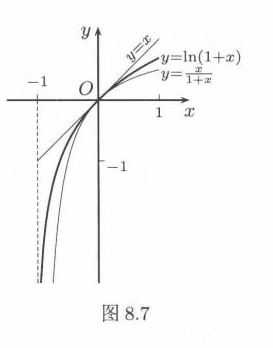
\includegraphics[width=.34\linewidth]{figures/upper/ch08/fig-8-7.png}
\end{center}

\begin{xremark}
回顾第二章中的不等式 (2.16)，即
\[
  \frac1{n+1}<\ln\left(1+\frac1n\right)<\frac1n,
\]
可以看到它只是本例题在 $x=1/n$ 时的特例。当时的不等式 (2.16) 来自于对数 $\ee$ 的研究，在那里只用了一个工具——平均值不等式。
\end{xremark}

Cauchy 中值定理在证明不等式中也有应用。

\begin{xexample}[8.5.2]
证明：对 $0<a<b\le\dfrac\pi2$，成立不等式
\[
  \frac{\sin a}{a}>\frac{\sin b}{b}.
\]
\end{xexample}
\begin{xproof}
这等价于证明函数 $\dfrac{\sin x}{x}$ 在区间 $(0,\dfrac\pi2]$ 上严格单调减少。（该函数的图像见图 4.2(a) 和 8.8(b)。）这里用 Cauchy 中值定理来作出证明。令 $f(x)=\sin x$，$g(x)=\sin\dfrac ba x$。从 Cauchy 中值定理知道存在 $\xi\in(0,a)$，使成立
\[
  \frac{\sin a}{\sin b}
  =\frac{f(a)-f(0)}{g(a)-g(0)}
  =\frac{f'(\xi)}{g'(\xi)}.
\]
由于 $f'(\xi)=\cos\xi$，$g'(\xi)=\dfrac ba\cos\dfrac ba\xi$，而 $\cos u$ 在 $0<u<\dfrac\pi2$ 上严格单调减少，因此就得到所要的结果
\[
  \frac{\sin a}{\sin b}
  =\frac ab\cdot\frac{\cos\xi}{\cos\frac ba\xi}>
  \frac ab.
\]
\end{xproof}

\begin{xremark}
这个例题的证明方法很多，这里再举出两个。

(1) 在区间 $(0,\pi/2]$ 上定义辅助函数 $F(x)=\sin x/x$，求导即可。

(2) 利用 8.2.2 小节的题 4，在 $[0,\pi/2]$ 上取 $f(x)=x$，$g(x)=\sin x$，由于 $f'(x)/g'(x)=\operatorname{sec}x$ 单调增加，因此 $x/\sin x$ 也单调增加。
\end{xremark}

利用单调性证明不等式的例子很多。一个典型例题就是

\begin{xexample}[8.5.3]
证明：在 $x>0$ 时，成立
\[
  \sin x>x-\frac{x^3}{6}.
\]
\end{xexample}
\begin{xproof}
令 $F(x)=\sin x-x+\dfrac{x^3}{6}$，则有 $F(0)=0$。因此只要证明当 $x>0$ 时成立 $F'(x)>0$，就可以从 $F$ 单调增加知道在 $x>0$ 时成立 $F(x)>0$。由于 $F'(0)=0$，又发现问题归结为证明 $F''(x)>0$（$x>0$）。由于 $F''(x)=-\sin x+x$，可见这已满足。由此反推即可。
\end{xproof}

证明不等式的另一个方法是将它转化为极值问题。下面就是一个典型例子（见 [30]），它在本书第十二章中有用。

\begin{xexample}[8.5.4]
设 $a\ge1$，证明：在 $x\in[0,a]$ 时成立不等式
\[
  0\le\ee^{-x}-\left(1-\frac xa\right)^a
  \le\frac{x^2}{a}\ee^{-x}.
\]
\end{xexample}
\begin{xproof}
先证明左边的不等式（这时只要 $a>0$）。将中间的表达式记为 $f(x)$，则只要证明 $f$ 在区间 $[0,a]$ 上的最小值非负即可。由于 $f(0)=0$，$f(a)=\ee^{-a}>0$，因此只要证明若 $f$ 有极值，则该极值非负。

若 $f'$ 没有零点，则无极值；若 $f'$ 有零点，记为 $\xi$，就有
\[
  f'(\xi)=-\ee^{-\xi}+\left(1-\frac\xi a\right)^{a-1}=0.
\]
由此即可计算出
\[
  f(\xi)=\ee^{-\xi}-\left(1-\frac\xi a\right)^a
  =\frac\xi a\cdot\ee^{-\xi}\ge0.
\]
因此左边不等式成立。对右边不等式的证明留作为 8.5.3 小节的练习题 16。
\end{xproof}

\begin{xremark}
在证明右边的不等式时，如果先乘以 $\ee^x$，则计算方便一些（见 [44]）。但这不是实质性的技巧。
\end{xremark}

下面是用一元微分学对平均值不等式的一个证明。它是由 Liouville（刘维尔）提出的（又为后人多次“发现”）。

\begin{xexample}[8.5.5]
用 Liouville 方法证平均值不等式，即对非负数 $x_1,x_2,\ldots,x_n$ 有
\[
  \frac{x_1+x_2+\cdots+x_n}{n}\ge\sqrt[n]{x_1x_2\cdots x_n},
\]
其中等号成立的充分必要条件是 $x_1=x_2=\cdots=x_n$。
\end{xexample}
\begin{xproof}
若在 $x_1,x_2,\ldots,x_n$ 中有 0 出现，则不等式已成立。同时也可看出成立等号的条件是其中每个数为 0。因此在下面设 $x_1,x_2,\ldots,x_n$ 全为正数。

用数学归纳法。在 $n=2$ 时已知成立。现设平均值不等式对 $n$ 已成立，讨论 $n+1$ 的情况。

构造辅助函数
\[
  y=\left(\frac{\sum_{i=1}^{n+1}x_i}{n+1}\right)^{n+1}
  -\prod_{i=1}^{n+1}x_i,
\]
并将 $x_{n+1}$ 看成是自变量，$y$ 是因变量。求导得到
\[
  \frac{\dd y}{\dd x_{n+1}}
  =\left(\frac{\sum_{i=1}^{n+1}x_i}{n+1}\right)^n
  -\prod_{i=1}^n x_i.
\]
可以看出这个导函数是 $(x_{n+1})$ 的严格单调增加函数。求出它的零点
\begin{equation}
  x_{n+1}=-\sum_{i=1}^n x_i+(n+1)\left(\prod_{i=1}^n x_i\right)^{1/n}.
  \tag{8.13}
  \label{eq:8.13}
\end{equation}
可见 $y$ 在该点取到最小值。记这个最小值为 $m$，则可以计算出
\begin{align*}
  m
  &=\prod_{i=1}^n x_i\left(\frac{\sum_{i=1}^{n+1}x_i}{n+1}-x_{n+1}\right)\\
  &=\prod_{i=1}^n x_i\left[
    \left(\prod_{i=1}^n x_i\right)^{1/n}
    +\sum_{i=1}^n x_i
    -(n+1)\left(\prod_{i=1}^n x_i\right)^{1/n}
  \right]\\
  &=\prod_{i=1}^n x_i\left[
    \sum_{i=1}^n x_i-n\left(\prod_{i=1}^n x_i\right)^{1/n}
  \right].
\end{align*}
对最后一式的第二个因子用归纳假设，可见最小值 $m\ge0$。因此得到 $y\ge m\ge0$，即已经得到了所要求证的不等式。

若在 $n+1$ 的平均值不等式中成立等号，则有 $y=0$，从而有 $y=m=0$。从 $m$ 的表达式和归纳假设可得 $x_1=x_2=\cdots=x_n$。又由 $y=m$ 可见 $x_{n+1}$ 满足等式 (8.13)，从而有 $x_{n+1}=x_1=\cdots=x_n$。
\end{xproof}

下面的 Jordan（若尔当）不等式是关于正弦函数的一个基本不等式。图 8.8(a) 是该不等式的几何意义，在图 8.8(b) 中作出了证 1 中的辅助函数 $\sin x/x$ 的图像。

\begin{xexample}[8.5.6（Jordan 不等式）]
设 $0\le x\le\dfrac\pi2$，则成立不等式
\[
  \sin x\ge\frac2\pi x.
\]
\end{xexample}
\begin{xproof}
\textbf{证 1}\quad 在 $x=0$ 时不等式已成立。对 $0<x\le\pi/2$ 可以引入辅助函数（见图 8.8(b)）
\[
  F(x)=\frac{\sin x}{x}.
\]
从例题 8.5.2 知 $F(x)$ 在 $(0,\pi/2]$ 上严格单调减少，从而在 $0<x\le\pi/2$ 时成立
\[
  F\left(\frac\pi2\right)=\frac2\pi\le F(x)=\frac{\sin x}{x}.
\]
这等价于所要求证的不等式。

\textbf{证 2}\quad 构造辅助函数
\[
  \varphi(x)=\sin x-\frac2\pi x,
\]
则只要证明在区间 $[0,\pi/2]$ 上函数 $\varphi(x)$ 非负。

在区间的两个端点上有
\[
  \varphi(0)=\varphi\left(\frac\pi2\right)=0.
\]
计算
\[
  \varphi'(x)=\cos x-\frac2\pi,
\]
可见 $\varphi'(x)$ 在区间 $[0,\pi/2]$ 上严格单调减少。由于 $\varphi'(0)>0$，$\varphi'(\pi/2)<0$，因此存在唯一的点 $\xi\in(0,\pi/2)$，使得 $\varphi'(\xi)=0$。这样就知道在 $0\le x\le\xi$ 时函数 $\varphi(x)$ 严格单调增加，因此有 $\varphi(x)\ge\varphi(0)=0$；而在 $\xi\le x\le\pi/2$ 时 $\varphi(x)$ 严格单调减少，因此有 $\varphi(x)\ge\varphi(\pi/2)=0$。这样就证明了在区间 $[0,\pi/2]$ 上处处成立 $\varphi(x)\ge0$。
\end{xproof}

\begin{center}
  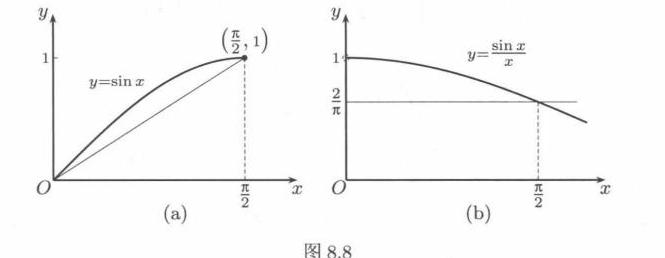
\includegraphics[width=.68\linewidth]{figures/upper/ch08/fig-8-8.png}
\end{center}

\begin{xremark}
从图 8.8(a) 可以想到，若 $y=\sin x$ 在 $[0,\pi/2]$ 上为上凸函数，则就可以得到 Jordan 不等式。从 $y''=-\sin x$ 可见这是对的。因此就得到了 Jordan 不等式的第三个证明。
\end{xremark}

用 Taylor 公式也是证明不等式的一种方法。例如下一个例题中就同时提供了关于函数 $\ln(1+x)$ 的许多不等式。

\begin{xexample}[8.5.7]
当 $x>0$ 时，证明：对每个正整数 $n$ 成立不等式
\[
  x-\frac{x^2}{2}+\frac{x^3}{3}-\cdots-\frac{x^{2n}}{2n}
  <\ln(1+x)<
  x-\frac{x^2}{2}+\frac{x^3}{3}-\cdots+\frac{x^{2n-1}}{2n-1}.
\]
\end{xexample}
\begin{xproof}
写出函数 $\ln(1+x)$ 的带 Lagrange 余项的 Maclaurin 公式：
\[
  \ln(1+x)=x-\frac{x^2}{2}+\frac{x^3}{3}-\cdots
  +(-1)^{n-1}\frac{x^n}{n}
  +\frac{(-1)^n}{n+1}\cdot\frac{x^{n+1}}{(1+\theta x)^{n+1}},
\]
其中 $0<\theta<1$。由于 $x>0$，右边的余项的符号由 $(-1)^n$ 决定。当 $n$ 为偶数时该项大于 0，而当 $n$ 为奇数时该项小于 0。这样就得到所要求证的不等式。
\end{xproof}

\subsection{用凸性证不等式}

这里的基本工具是 Jensen 不等式 (8.11)（见命题 8.4.7）。在那里已经提到，该不等式对所有下凸函数成立，而并不要求二阶可微的条件。但用二阶导数的符号来验证一个给定函数是否下凸还是一个很实际的方法。

在下面的前三个不等式统称为经典不等式。由于它们在数学中的重要性，均作为命题给出。第一个不等式即平均值不等式（命题 1.3.3）的推广。

\begin{xtheorem}[8.5.1（广义的算术平均值－几何平均值不等式）]
设有非负数 $x_1,\ldots,x_n$ 和正数 $\lambda_1,\ldots,\lambda_n$，且 $\lambda_1+\cdots+\lambda_n=1$，则成立不等式
\begin{equation}
  \prod_{k=1}^n x_k^{\lambda_k}\le\sum_{k=1}^n\lambda_kx_k,
  \tag{8.14}
  \label{eq:8.14}
\end{equation}
其中当且仅当 $x_1=x_2=\cdots=x_n$ 时成立等号。
\end{xtheorem}
\begin{xproof}
令 $f(u)=-\ln u$，$u>0$。由于 $f''(u)=1/u^2>0$，因此 $f(u)$ 是严格下凸函数（用命题 8.4.6）。用 Jensen 不等式 (8.11) 得到
\[
  -\ln\left(\sum_{k=1}^n\lambda_kx_k\right)
  \le-\sum_{k=1}^n\lambda_k\ln x_k.
\]
移项并利用对数函数的单调性，即可得到所要求证的不等式。关于其中成立等号的条件已在命题 8.4.7 中得到证明。
\end{xproof}

\begin{xremark}
若取 $\lambda_i=1/n$，$i=1,2,\ldots,n$，就得到普通的平均值不等式。此外，与平均值不等式类似，有许多不同的方法可以证明以上的广义平均值不等式。
\end{xremark}

第二个要介绍的 Hölder（赫尔德）不等式是在第一章中的 Cauchy 不等式（见命题 1.3.5）的推广，它在数学的许多领域中起重要作用，也可以用于证明广义的平均值不等式。

\begin{xtheorem}[8.5.2（Hölder 不等式）]
设 $x_1,x_2,\ldots,x_n$ 和 $y_1,y_2,\ldots,y_n$ 均为非负数，又有 $p>1$，$q>1$，且满足（共轭）条件
\[
  \frac1p+\frac1q=1,
\]
则成立不等式
\begin{equation}
  \sum_{k=1}^n x_ky_k
  \le\left(\sum_{k=1}^n x_k^p\right)^{1/p}
  \left(\sum_{k=1}^n y_k^q\right)^{1/q},
  \tag{8.15}
  \label{eq:8.15}
\end{equation}
其中成立等号的充分必要条件是数组 $x_1^p,x_2^p,\ldots,x_n^p$ 和 $y_1^q,y_2^q,\ldots,y_n^q$ 成比例。
\end{xtheorem}
\begin{xproof}
先对于至少有一个数组中的每个数都大于 0 的情况作出证明。为确定起见，不妨设 $y_1,y_2,\ldots,y_n$ 中的每个数都大于 0，则可证明如下。

取函数 $f(u)=u^p$，$u\ge0$。由于 $f''(u)=p(p-1)u^{p-2}\ge0$，因此 $f(u)$ 是严格下凸函数。令
\[
  \lambda_k=\frac{y_k^q}{\sum_{i=1}^n y_i^q},
  \qquad
  u_k=x_ky_k^{1-q},
  \qquad k=1,2,\ldots,n,
\]
并代入 Jensen 不等式 (8.11)，就有
\begin{equation}
  \left(\frac{\sum_{k=1}^n x_ky_k}{\sum_{k=1}^n y_k^q}\right)^p
  \le\sum_{k=1}^n\left[
    \frac{y_k^q}{\sum_{i=1}^n y_i^q}\cdot(x_ky_k^{1-q})^p
  \right]
  =\frac{\sum_{k=1}^n x_k^p}{\sum_{k=1}^n y_k^q}.
  \tag{8.16}
  \label{eq:8.16}
\end{equation}
其中利用了 $p,q$ 满足条件 $p+q-pq=0$。两边开 $p$ 次根，并略加整理即得
\[
  \sum_{k=1}^n x_ky_k
  \le\left(\sum_{k=1}^n x_k^p\right)^{1/p}
  \left(\sum_{k=1}^n y_k^q\right)^{1-1/p}
  =\left(\sum_{k=1}^n x_k^p\right)^{1/p}
  \left(\sum_{k=1}^n y_k^q\right)^{1/q}.
\]
关于在 Hölder 不等式中成立等号的条件也可从 Jensen 不等式得到，即 $u_1=u_2=\cdots=u_n$。从 $u_k$ 的表达式，可以将这个条件写成为：存在常数 $C$，使成立 $x_k^p=Cy_k^q$，$k=1,2,\ldots,n$。由不等式 (8.15) 的对称性，对 $x_1,x_2,\ldots,x_n$ 中每个数大于 0 的情况的证明完全相同。而在不等式中成立等号的条件可统一写成为：存在两个不全为 0 的数 $\lambda$ 和 $\mu$，使成立
\begin{equation}
  \lambda x_k^p=\mu y_k^q,\qquad k=1,2,\ldots,n.
  \tag{8.17}
  \label{eq:8.17}
\end{equation}
现在讨论其余情况，即在两个数组中都有某些数为 0 的情况。

若有一个数组中的数全为 0，则不等式 (8.15) 成立等号，且只要在 $\lambda$ 和 $\mu$ 中取一个为 0，就可以使得 (8.17) 成立。

对于两个数组都有部分数为 0，但不是全为 0 的情况，可以取定 $y_1,y_2,\ldots,y_n$，将其中为 0 的数（以及在数组 $x_1,x_2,\ldots,x_n$ 中相同下标的数）剔除，就可以归结为前面的情况来证明。又从不等式 (8.15) 可直接看出，如有某个 $y_k=0$，且在不等式中成立等号，则相应地也一定有 $x_k=0$。因此条件 (8.17) 仍然成立。
\end{xproof}

第三个不等式就是下面的 Minkowski（闵可夫斯基）不等式。当其中的参数 $p=2$ 时就是 $n$ 维 Euclid（欧几里得）空间的三点不等式（或三角形不等式）。

\begin{xtheorem}[8.5.3（Minkowski 不等式）]
设 $x_1,x_2,\ldots,x_n$ 和 $y_1,y_2,\ldots,y_n$ 均为非负数，又有 $p>1$，则成立不等式
\begin{equation}
  \left[\sum_{k=1}^n(x_k+y_k)^p\right]^{1/p}
  \le\left(\sum_{k=1}^n x_k^p\right)^{1/p}
  +\left(\sum_{k=1}^n y_k^p\right)^{1/p},
  \tag{8.18}
  \label{eq:8.18}
\end{equation}
当且仅当数组 $x_1,x_2,\ldots,x_n$ 和 $y_1,y_2,\ldots,y_n$ 成比例时成立等号。
\end{xtheorem}
\begin{xproof}
只需对 $p>1$ 作出证明。令
\[
  f(u)=\left(1-u^{1/p}\right)^p,\qquad0<u<1,
\]
并计算导数
\[
  f'(u)=-\left(1-u^{1/p}\right)^{p-1}u^{1/p-1},
\]
\[
  f''(u)=\left(1-\frac1p\right)\left(1-u^{1/p}\right)^{p-2}u^{1/p-2}.
\]
可见 $f(u)$ 是严格下凸函数。令
\[
  \lambda_k=\frac{(x_k+y_k)^p}{\sum_{i=1}^n(x_i+y_i)^p},
  \qquad
  u_k=\left(\frac{x_k}{x_k+y_k}\right)^p,
\]
这里假定每个 $x_k+y_k\ne0$（$k=1,2,\ldots,n$）成立。这使得每个 $u_k$ 有意义，同时保证 $\lambda_k>0$ 成立。

将上述 $\lambda_k,u_k$（$k=1,2,\ldots,n$）代入 Jensen 不等式 (8.11)，就有
\[
  \left[
    1-\left(\sum_{k=1}^n\frac{x_k^p}{\sum_{i=1}^n(x_i+y_i)^p}\right)^{1/p}
  \right]^p
  \le\sum_{k=1}^n\frac{(x_k+y_k)^p}{\sum_{i=1}^n(x_i+y_i)^p}
  \left(1-\frac{x_k}{x_k+y_k}\right)^p
  =\frac{\sum_{k=1}^n y_k^p}{\sum_{k=1}^n(x_k+y_k)^p}.
\]
在上式两边开 $p$ 次根并加以整理，就可得到所要的 Minkowski 不等式。

若在该不等式中成立等号，则从 Jensen 不等式知道有 $u_1=u_2=\cdots=u_n$。由此可得到两个数组成比例的结论。

最后，若对某些（但不是所有）$k$ 有 $x_k+y_k=0$，则由于 $x_k\ge0$ 和 $y_k\ge0$，就有 $x_k=y_k=0$。因此在将它们剔除后就可以归结为前面的情况，而且并不影响在等号成立时两个数组成比例的结论。对于两个数组全由 0 组成的极端情况，命题明显成立。
\end{xproof}

\begin{xremark}
\textbf{注 1}\quad 在 $p=2$ 时两个数组中的数的非负性要求可以取消，但这时成立等号的条件应当改写为：存在两个不全为 0 的非负数 $\lambda$ 和 $\mu$，使得成立
\[
  \lambda x_k=\mu y_k,\qquad k=1,2,\ldots,n.
\]
读者可以思考这个条件在 $n$ 维 Euclid 空间中的几何意义。

\textbf{注 2}\quad 证明 Minkowski 不等式的方法很多，例如用数学归纳法或 Hölder 不等式都可以证明它。
\end{xremark}

下面的不等式是第一章中的 Bernoulli 不等式（命题 1.3.1）的推广。它也可以用凸性来证明，读者如果对比两者的结论和所用的工具，就可以对于自己已经向前走了多远有一个了解。

\begin{xtheorem}[8.5.4（Bernoulli 不等式）]
在 $x>-1$ 时，对于 $0<\alpha<1$ 成立不等式
\[
  (1+x)^\alpha\le1+\alpha x,
\]
而对于 $\alpha<0$ 和 $\alpha>1$ 则成立相反的不等式
\[
  (1+x)^\alpha\ge1+\alpha x,
\]
而且在这些不等式中仅当 $x=0$ 时成立等号。
\end{xtheorem}
\begin{xproof}
对于函数 $f(x)=(1+x)^\alpha$ 计算导数：
\[
  f'(x)=\alpha(1+x)^{\alpha-1},
  \qquad
  f''(x)=\alpha(\alpha-1)(1+x)^{\alpha-2},
\]
就可以知道，当 $0<\alpha<1$ 时 $f(x)$ 是严格上凸函数，而当 $\alpha<0$ 和 $\alpha>1$ 时 $f(x)$ 是严格下凸函数。另一方面 $y=1+\alpha x$ 是曲线 $y=f(x)$ 在点 $(0,1)$ 处的切线。应用命题 8.4.5，就有所要的不等式，包括成立等号的条件。
\end{xproof}

\subsection{练习题}

\begin{xexercise}[1]
证明：当 $x>1$ 时，成立
  \[
    \ln x>\frac{2(x-1)}{x+1}.
  \]
\end{xexercise}
\begin{xsolution}
令
\[
  F(x)=\ln x-\frac{2(x-1)}{x+1}.
\]
则 $F(1)=0$，且
\[
  F'(x)=\frac1x-\frac4{(x+1)^2}
  =\frac{(x-1)^2}{x(x+1)^2}>0\qquad(x>1).
\]
故 $F(x)>0$，即所证不等式成立。
\end{xsolution}


\begin{xexercise}[2]
证明：当 $0<a<b$ 时，成立不等式
  \[
    a\ln a+b\ln b>(a+b)\cdot[\ln(a+b)-\ln2].
  \]
\end{xexercise}
\begin{xsolution}
函数 $h(x)=x\ln x$ 在 $(0,+\infty)$ 上严格下凸，因为 $h''(x)=1/x>0$。由 Jensen 不等式，且 $a\ne b$，
\[
  \frac{a\ln a+b\ln b}{2}>
  \frac{a+b}{2}\ln\frac{a+b}{2}.
\]
两边乘以 2 即得
\[
  a\ln a+b\ln b>(a+b)[\ln(a+b)-\ln2].
\]
\end{xsolution}


\begin{xexercise}[3]
证明：对任意 $0<x_1<x_2$，成立不等式
  \[
    \frac{x_2-x_1}{x_2}<\ln\frac{x_2}{x_1}<\frac{x_2-x_1}{x_1}.
  \]
\end{xexercise}
\begin{xsolution}
令 $t=(x_2-x_1)/x_1>0$，则 $x_2/x_1=1+t$。例题 8.5.1 给出
\[
  \frac{t}{1+t}<\ln(1+t)<t.
\]
代回即为
\[
  \frac{x_2-x_1}{x_2}<\ln\frac{x_2}{x_1}
  <\frac{x_2-x_1}{x_1}.
\]

\textbf{另解}\quad 对 $\ln x$ 在区间 $[x_1,x_2]$ 使用 Lagrange 中值定理，存在 $\xi\in(x_1,x_2)$ 使
\[
  \frac{\ln x_2-\ln x_1}{x_2-x_1}=\frac1\xi.
\]
由于 $x_1<\xi<x_2$，有
\[
  \frac1{x_2}<\frac1\xi<\frac1{x_1},
\]
两边乘以 $x_2-x_1>0$ 即得所证双边不等式。
\end{xsolution}


\begin{xexercise}[4]
证明以下不等式：
  \begin{enumerate}[label=(\arabic*)]
    \item $\displaystyle a^{\frac{x_1+x_2+\cdots+x_n}{n}}
    \le\frac1n(a^{x_1}+a^{x_2}+\cdots+a^{x_n})$，其中 $a>0$；
    \item $\displaystyle\left(\frac{x_1+x_2+\cdots+x_n}{n}\right)^p
    \le\frac1n(x_1^p+x_2^p+\cdots+x_n^p)$，其中 $p>1$；
    \item 当 $x_1,x_2,\ldots,x_n>0$ 时，
    \[
      \frac{x_1+x_2+\cdots+x_n}{n}
      \le\left(x_1^{x_1}x_2^{x_2}\cdots x_n^{x_n}\right)^{\frac1{x_1+x_2+\cdots+x_n}}.
    \]
  \end{enumerate}
\end{xexercise}
\begin{xsolution}
\begin{enumerate}[label=(\arabic*)]
  \item 函数 $u\mapsto a^u=\ee^{u\ln a}$ 为下凸函数（$a=1$ 时为常值），故 Jensen 不等式给出
  \[
    a^{(x_1+\cdots+x_n)/n}\le\frac1n\sum_{i=1}^n a^{x_i}.
  \]

  \item 在使 $x_i^p$ 为实数的通常非负变量范围内，$u\mapsto u^p$（$p>1$）下凸，因此
  \[
    \left(\frac{x_1+\cdots+x_n}{n}\right)^p
    \le\frac1n\sum_{i=1}^n x_i^p.
  \]

  \item 函数 $h(u)=u\ln u$ 在 $(0,+\infty)$ 上严格下凸。记
  \[
    S=\sum_{i=1}^n x_i,\qquad \bar x=\frac Sn.
  \]
  Jensen 不等式给出
  \[
    \frac1n\sum x_i\ln x_i\ge\bar x\ln\bar x.
  \]
  乘以 $n/S$ 后指数化，得到
  \[
    \frac Sn\le
    \exp\left(\frac1S\sum x_i\ln x_i\right)
    =\left(\prod x_i^{x_i}\right)^{1/S}.
  \]
\end{enumerate}
\end{xsolution}


\begin{xexercise}[5]
证明：对于 $0<\alpha<1$ 和 $x>0$ 成立 $x^\alpha-\alpha x+\alpha-1\le0$，而当 $\alpha>1$ 时不等式反向成立。
\end{xexercise}
\begin{xsolution}
在 Bernoulli 不等式中令 $u=x-1>-1$。当 $0<\alpha<1$ 时
\[
  x^\alpha=(1+u)^\alpha\le1+\alpha u=\alpha x+1-\alpha,
\]
即
\[
  x^\alpha-\alpha x+\alpha-1\le0.
\]
当 $\alpha>1$ 时 Bernoulli 不等式反向，故结论也反向。
\end{xsolution}


\begin{xexercise}[6]
从命题 2.5.1 已知，对每个 $n\in\NN_+$，成立不等式
  \[
    \left(1+\frac1n\right)^n\le\ee\le\left(1+\frac1n\right)^{n+1}.
  \]
  作为进一步的发展，求出最大的 $\alpha$ 和最小的 $\beta$，使得
  \[
    \left(1+\frac1n\right)^{n+\alpha}\le\ee\le
    \left(1+\frac1n\right)^{n+\beta},\qquad\forall n\in\NN_+.
  \]
  （本题与例题 8.2.3 有联系。）
\end{xexercise}
\begin{xsolution}
所求条件等价于
\[
  \alpha\le A_n\le\beta,
  \qquad
  A_n=\frac1{\ln(1+1/n)}-n.
\]
把 $n$ 暂看作连续变量 $x>0$。可证明 $A(x)$ 严格增加。事实上令 $t=1/x$，只需用
\[
  \ln(1+t)<\frac{t}{\sqrt{1+t}},\qquad t>0,
\]
而该式可由两边之差求导得到。于是
\[
  \inf_{n\ge1}A_n=A_1=\frac1{\ln2}-1.
\]
另一方面由
\[
  \ln(1+1/n)=\frac1n-\frac1{2n^2}+\bigO(n^{-3})
\]
得
\[
  \lim_{n\to\infty}A_n=\frac12.
\]
因此最大的 $\alpha$ 与最小的 $\beta$ 分别是
\[
  \boxed{\alpha=\frac1{\ln2}-1,\qquad \beta=\frac12}.
\]
\end{xsolution}


\begin{xexercise}[7]
证明：对 $0<a<b$，成立以下不等式：
  \[
    a<\frac2{\frac1a+\frac1b}<\sqrt{ab}<\frac{b-a}{\ln b-\ln a}<\frac{a+b}{2}
    <\sqrt{\frac{a^2+b^2}{2}}<b.
  \]
\end{xexercise}
\begin{xsolution}
依次记调和、几何、对数、算术、平方平均值为 $H,G,L,A,Q$。显然 $a<H$。由
\[
  (\sqrt a-\sqrt b)^2>0
\]
可得 $H<G$。

令 $u=\sqrt{b/a}>1$。不等式 $G<L$ 等价于
\[
  2\ln u<u-\frac1u.
\]
右减左的导数为 $(u-1)^2/u^2>0$，且在 $u=1$ 为 0，故成立。

由题 1 对 $x=b/a>1$ 应用
\[
  \ln x>\frac{2(x-1)}{x+1},
\]
得到 $L<A$。而
\[
  A<Q
\]
是严格的均方根－算术平均值不等式，$Q<b$ 由 $a^2<b^2$ 立即得到。因此
\[
  a<H<G<L<A<Q<b.
\]
\end{xsolution}


\begin{xexercise}[8]
对于 $2n$ 个正数 $x_1,x_2,\ldots,x_n$ 和 $\lambda_1,\lambda_2,\ldots,\lambda_n$，且 $\lambda_1+\lambda_2+\cdots+\lambda_n=1$，定义加权的 $t$ 阶平均值（或 $t$ 阶和）为
  \[
    M_t(x,\lambda)=\left(\sum_{i=1}^n\lambda_i x_i^t\right)^{1/t}.
  \]
  它在 $t=-1$ 时为调和平均值，$t=1$ 时为算术平均值，$t=2$ 时为平方平均值（即均方根值）。又若在 $t=0,+\infty,-\infty$ 时用极限作补充定义，则在 $t=0$ 时为几何平均值，$t=+\infty$ 时为 $\max\{x\}$，$t=-\infty$ 时为 $\min\{x\}$。这样就使 $M_t(x,\lambda)$ 在 $-\infty\le t\le+\infty$ 上处处有定义。证明：$M_t(x,\lambda)$ 是 $t$ 的单调增加函数，在 $n>1$ 且 $x_1,x_2,\ldots,x_n$ 不全相等时为 $t$ 的严格单调增加函数。
\end{xexercise}
\begin{xsolution}
先取有限的 $r<s$。若 $0<r<s$，令 $p=s/r>1$，对正数 $x_i^r$ 用加权幂平均（或 Jensen）得
\[
  \left(\sum\lambda_i x_i^r\right)^{1/r}
  \le
  \left(\sum\lambda_i x_i^s\right)^{1/s}.
\]
若 $r<s<0$，对 $1/x_i$ 使用前述正指数情形即可。若 $r<0<s$，分别与 $M_0=\prod x_i^{\lambda_i}$ 比较即可；$r=0$ 由极限连接。

当 $n>1$ 且 $x_i$ 不全相等时，所用 Jensen/幂平均不等式均为严格不等式，所以 $M_t$ 严格增加。最后
\[
  \lim_{t\to+\infty}M_t=\max_i x_i,
  \qquad
  \lim_{t\to-\infty}M_t=\min_i x_i,
\]
与题中的补充定义一致，故结论在整个扩充参数区间成立。
\end{xsolution}


\begin{xexercise}[9]
证明：若将 Minkowski 不等式 (8.18) 中的参数 $p\ge1$ 的条件改为 $0<p<1$，则不等式反向成立。
\end{xexercise}
\begin{xsolution}
设 $0<p<1$，并记
\[
  A=\left(\sum x_k^p\right)^{1/p},
  \qquad
  B=\left(\sum y_k^p\right)^{1/p}.
\]
若 $A,B>0$，令 $u_k=x_k/A$，$v_k=y_k/B$，$\lambda=A/(A+B)$，$\mu=B/(A+B)$。由于 $t^p$ 在非负半轴上为上凸函数，
\[
  \sum(\lambda u_k+\mu v_k)^p
  \ge\lambda\sum u_k^p+\mu\sum v_k^p=1.
\]
因此
\[
  \left(\sum(x_k+y_k)^p\right)^{1/p}\ge A+B,
\]
即 Minkowski 不等式反向。$A=0$ 或 $B=0$ 时结论直接成立。
\end{xsolution}


\begin{xexercise}[10]
证明 Young（杨氏）不等式：若 $x,y\ge0$，$p,q>1$，$\dfrac1p+\dfrac1q=1$，则成立不等式
  \[
    x^{1/p}y^{1/q}\le\frac xp+\frac yq.
  \]
\end{xexercise}
\begin{xsolution}
对非负数 $x,y$ 应用权为 $1/p,1/q$ 的加权算术－几何平均值不等式：
\[
  \frac xp+\frac yq
  \ge x^{1/p}y^{1/q}.
\]
这就是 Young 不等式。等号当且仅当 $x=y$。
\end{xsolution}


\begin{xexercise}[11]
试用 Young 不等式证明：
  \begin{enumerate}[label=(\arabic*)]
    \item 广义的算术平均值－几何平均值不等式；
    \item Hölder 不等式。
  \end{enumerate}
\end{xexercise}
\begin{xsolution}
\begin{enumerate}[label=(\arabic*)]
  \item 对两个数，Young 不等式正是权重为 $1/p$、$1/q$ 的加权 AM--GM。对多个有理权重反复使用二元形式即可得到广义 AM--GM；一般实权重再由连续性逼近得到。

  \item 记
  \[
    X=\left(\sum x_k^p\right)^{1/p},
    \qquad
    Y=\left(\sum y_k^q\right)^{1/q}.
  \]
  若 $XY=0$ 则显然。否则对每个 $k$ 将 Young 不等式用于
  \[
    \left(\frac{x_k}{X}\right)^p,
    \qquad
    \left(\frac{y_k}{Y}\right)^q,
  \]
  得
  \[
    \frac{x_ky_k}{XY}
    \le\frac1p\frac{x_k^p}{X^p}
       +\frac1q\frac{y_k^q}{Y^q}.
  \]
  对 $k$ 求和，右端为 $1/p+1/q=1$，故
  \[
    \sum x_ky_k\le XY,
  \]
  即 Hölder 不等式。
\end{enumerate}
\end{xsolution}


\begin{xexercise}[12]
设 $f$ 和 $\varphi$ 在 $x\ge a$ 时可微，$f(a)=\varphi(a)$，且当 $x\ge a$ 时，成立 $|f'(x)|\le\varphi'(x)$，证明：当 $x\ge a$ 时，成立
  \[
    |f(x)-f(a)|\le\varphi(x)-\varphi(a).
  \]
\end{xexercise}
\begin{xsolution}
由 $|f'|\le\varphi'$ 可知 $\varphi'\ge0$，且
\[
  (\varphi-f)'=\varphi'-f'\ge0,
  \qquad
  (\varphi+f)'=\varphi'+f'\ge0.
\]
因此对 $x\ge a$，利用 $f(a)=\varphi(a)$，
\[
  \varphi(x)-\varphi(a)\ge f(x)-f(a),
\]
同时
\[
  \varphi(x)-\varphi(a)\ge-[f(x)-f(a)].
\]
合并即得
\[
  |f(x)-f(a)|\le\varphi(x)-\varphi(a).
\]
\end{xsolution}


\begin{xexercise}[13]
设 $f$ 满足 $f(1)=1$，且当 $x\ge1$ 时有
  \[
    f'(x)=\frac1{x^2+f^2(x)}.
  \]
  证明：极限 $\displaystyle\lim_{x\to+\infty}f(x)$ 存在，且小于 $1+\pi/4$。
\end{xexercise}
\begin{xsolution}
因 $f'(x)>0$，$f$ 在 $[1,+\infty)$ 上严格增加，故 $f(x)\ge1$。于是
\[
  0<f'(x)=\frac1{x^2+f(x)^2}<\frac1{x^2+1}\qquad(x>1).
\]
令
\[
  \varphi(x)=1+\arctan x-\frac\pi4.
\]
则 $\varphi(1)=f(1)=1$ 且 $f'(x)<\varphi'(x)$，故由导数比较
\[
  1<f(x)<1+\arctan x-\frac\pi4<1+\frac\pi4.
\]
所以 $f$ 单调增加且有上界，极限
\[
  L=\lim_{x\to+\infty}f(x)
\]
存在。又由微分方程
\[
  L-1
  =\int_1^{+\infty}\frac{\dd t}{t^2+f(t)^2}.
\]
对 $t>1$ 有 $f(t)>1$，故被积函数严格小于 $1/(t^2+1)$。例如先在 $[1,2]$ 上积分即可得到严格差额，而在 $[2,+\infty)$ 上仍保持不大于，因而
\[
  L-1
  <\int_1^{+\infty}\frac{\dd t}{t^2+1}
  =\frac\pi4.
\]
所以
\[
  \boxed{\displaystyle\lim_{x\to+\infty}f(x)<1+\frac\pi4}.
\]
\end{xsolution}


\begin{xexercise}[14]
设 $A=(a_{ij})_{1\le i,j\le n}$ 是每行每列的和均等于 1 的非负元素矩阵，又有
  \[
    \begin{pmatrix}y_1\\\vdots\\y_n\end{pmatrix}
    =A\begin{pmatrix}x_1\\\vdots\\x_n\end{pmatrix},
  \]
  其中两个向量的所有元素也都是非负数，证明：$y_1\cdots y_n\ge x_1\cdots x_n$。
\end{xexercise}
\begin{xsolution}
对每个 $i$，有
\[
  y_i=\sum_{j=1}^n a_{ij}x_j,
  \qquad a_{ij}\ge0,\quad \sum_j a_{ij}=1.
\]
由加权 AM--GM，
\[
  y_i\ge\prod_{j=1}^n x_j^{a_{ij}}.
\]
对 $i$ 相乘，并利用每列和也为 1，得到
\[
  \prod_{i=1}^n y_i
  \ge\prod_{j=1}^n x_j^{\sum_i a_{ij}}
  =\prod_{j=1}^n x_j.
\]
若某些 $x_j=0$，右端为 0，结论仍直接成立。
\end{xsolution}


\begin{xexercise}[15]
若记
  \[
    T_n(x)=x-\frac1{3!}x^3+\cdots+\frac{(-1)^n}{(2n+1)!}x^{2n+1}
    =\sum_{k=0}^n\frac{(-1)^k}{(2k+1)!}x^{2k+1}
  \]
  % SOURCE-ERR: 原书右端求和下标印作 k=1，与左端首项 x 不一致；此处按显然应为 k=0 修正。
  为 $\sin x$ 在 $x=0$ 处的 $2n+1$ 次 Taylor 多项式，证明：
  \[
    \sin x>\sum_{k=0}^n\frac{(-1)^k}{(2k+1)!}x^{2k+1},
    \quad\text{其中 }x>0,\ n\text{ 为奇数},
  \]
  \[
    \sin x<\sum_{k=0}^n\frac{(-1)^k}{(2k+1)!}x^{2k+1},
    \quad\text{其中 }x>0,\ n\text{ 为偶数}.
  \]
  （例题 8.5.3 是本题的一个特例。类似地，可以建立关于 $\cos x$ 的结果。）
\end{xexercise}
\begin{xsolution}
记
\[
  R_n(x)=\sin x-T_n(x).
\]
有 $R_n(0)=R_n'(0)=0$，并且
\[
  R_n''(x)=-R_{n-1}(x).
\]
从 $R_0(x)=\sin x-x<0$（$x>0$）开始归纳。若 $R_{n-1}$ 在 $x>0$ 上符号为 $(-1)^n$，则 $R_n''$ 的符号为 $(-1)^{n+1}$。由 $R_n'(0)=R_n(0)=0$ 两次利用单调性可知 $R_n$ 本身也具有符号 $(-1)^{n+1}$。因此 $n$ 为奇数时 $R_n>0$，$n$ 为偶数时 $R_n<0$，恰为题中两式。
\end{xsolution}


\begin{xexercise}[16]
证明例题 8.5.4 中右边的不等式。
\end{xexercise}
\begin{xsolution}
要证
\[
  \ee^{-x}-\left(1-\frac xa\right)^a
  \le\frac{x^2}{a}\ee^{-x},
  \qquad 0\le x\le a,\ a\ge1.
\]
乘以 $\ee^x$ 后等价于
\[
  1-\ee^x\left(1-\frac xa\right)^a\le\frac{x^2}{a}.
\]
若 $x\ge\sqrt a$，右端不小于 1，而左端不大于 1，结论成立。

以下设 $0\le x<\sqrt a$。此时两边移项后都为正，只需证明
\[
  \ee^x\left(1-\frac xa\right)^a\ge1-\frac{x^2}{a}.
\]
取对数，令
\[
  H(x)=x+a\ln\left(1-\frac xa\right)
       -\ln\left(1-\frac{x^2}{a}\right).
\]
有 $H(0)=0$，直接化简得
\[
  H'(x)=
  \frac{x[(x-1)^2+a-1]}{(a-x)(a-x^2)}\ge0.
\]
故 $H(x)\ge0$，所需不等式成立。
\end{xsolution}


\section{函数作图}

在用微分学知识作函数 $y=f(x)$ 的图像时，应注意以下基本内容：

1. 基本初等函数的图像（中学数学中的基本内容）。

2. 多项式函数 $y=a_0x^n+a_1x^{n-1}+\cdots+a_n$ 的图像，特别是其中 $n=2,3$ 时的所有可能情况，以及 $n$ 为奇数和偶数时的各种可能情况。

3. 利用某个函数的已知图像经过简单变换得到新的图像的方法。这里的内容有，设已知 $y=f(x)$ 的图像，求以下函数的图像：
\begin{enumerate}[label=(\arabic*)]
  \item $y=f(-x)$；
  \item $y=-f(x)$；
  \item $y=-f(-x)$；
  \item $x=f(y)$；
  \item $y=f(x+a)$；
  \item $y=f(kx)$；
  \item $y=kf(x)$；
  \item $y=f(x)+a$；
  \item $y=|f(x)|$。
\end{enumerate}

4. 已知函数 $y=f(x)$ 和 $y=g(x)$ 的图像，作出函数 $y=f(x)+g(x)$，$y=f(x)-g(x)$，$y=f(x)\cdot g(x)$ 的图像。

\begin{xremark}
熟练掌握以上技巧对于作出函数的大致图像（即所谓作草图）有很大帮助。作草图时不需要微分学的知识，但是若能将作草图的方法与微分学相结合，就可以既迅速又准确地作出函数的图像。
\end{xremark}

对于函数 $y=f(x)$ 的一般作图步骤在教科书中均有介绍，这里不必重复。对于用参数方程表示的函数 $x=x(t),y=y(t)$ 的作图问题，一般是先分别作出 $x=x(t)$ 和 $y=y(t)$ 的图像，然后再拼成为一张图（见下面的例题）。对于用方程 $F(x,y)=0$ 确定的隐函数，往往引入参数 $t$ 而转化为上一问题。

\subsection{例题}

\begin{xexample}[8.6.1]
作出用参数方程
\[
  x=2t-4t^3,\qquad y=t^2-3t^4
\]
给出的曲线图像。
\end{xexample}
\begin{xsolution}
$x(t)$ 和 $y(t)$ 只是 $t$ 的三次和四次多项式，容易分别作出它们的图像如图 8.9(a)、8.9(b) 所示：

\begin{center}
  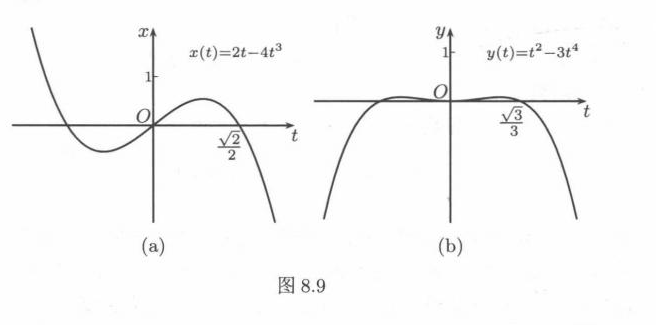
\includegraphics[width=.70\linewidth]{figures/upper/ch08/fig-8-9.png}
\end{center}

关于三次多项式 $x(t)=2t-4t^3$ 的主要分析如下：$x(t)$ 是奇函数；导函数 $x'_t=2-12t^2$ 的零点为 $t=\pm1/\sqrt6$，其中 $-1/\sqrt6\approx-0.4082$ 是极小值点，极小值为 $-2\sqrt6/9\approx-0.5443$，$1/\sqrt6\approx0.4082$ 是极大值点，极大值为 $2\sqrt6/9\approx0.5443$；$x(t)$ 有三个零点：0 和 $\pm\sqrt2/2\approx\pm0.7071$。

关于四次多项式 $y=t^2-3t^4$ 的主要分析如下：$y(t)$ 是偶函数，导函数 $y'_t=2t-12t^3$ 有三个零点：0 和 $\pm1/\sqrt6\approx\pm0.4082$，其中 $t=0$ 为极小值点，极小值为 0，其他两个零点是 $y(t)$ 的极大值点，极大值为 $1/12\approx0.0833$；$y(t)$ 除了二重零点 0 之外还有两个零点：$\pm\sqrt3/3\approx\pm0.5774$。

现在已经可以将以上分析合并以得到所要求的参数方程的图像，这就是图 8.10，其中参数 $t$ 的变化范围为从 $-0.95$ 到 $0.95$。

\begin{center}
  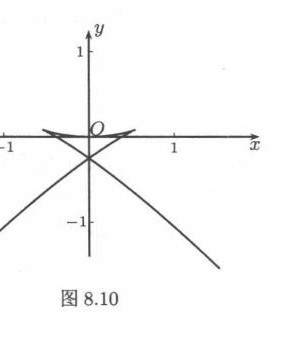
\includegraphics[width=.36\linewidth]{figures/upper/ch08/fig-8-10.png}
\end{center}

图 8.10 的作法如下。首先，当 $x$ 换为 $-x$ 时，对应的参数值 $t$ 也反号，但 $y$ 是 $t$ 的偶函数，从而可见在 $xOy$ 坐标系中曲线关于 $y$ 轴对称。因此以下只需讨论参数 $t>0$ 的情况。根据 6.2.3 小节的参数方程求导法则，就有
\[
  \frac{\dd y}{\dd x}=\frac{y'_t}{x'_t}
  =t\cdot\frac{1-6t^2}{1-6t^2},
\]
因此当 $t\ne1/\sqrt6\approx0.4082$ 时，就得到
\[
  \frac{\dd y}{\dd x}=t.
\]
从前面对 $x'_t$ 和 $y'_t$ 的分析已经知道当 $t=1/\sqrt6$ 时这两个导数均为 0，我们将这样的点称为奇点。这是本例中的主要困难。由于关于 $y$ 轴对称，因此有两个奇点：$(\pm2\sqrt6/9,1/12)$，两个坐标的近似值为 $\pm0.5443$ 和 $0.0833$。

当 $t$ 从 0 变化到 $1/\sqrt6$ 时，由于 $y'_x=t$，而 $x(t)$ 和 $y(t)$ 均为 $t$ 的严格单调增加函数，因此可以知道 $y$ 是 $x$ 的严格单调增加函数。又由于导函数 $y'_x$ 也是 $x$ 的严格单调增加函数，因此 $y=y(x)$ 是下凸函数。

从同样的分析可以知道，当 $t$ 从 $1/\sqrt6$ 起增加时，$y$ 是 $x$ 的严格单调增加函数，而且是上凸函数。

从前面已经得到的导数公式可以知道，有
\[
  \lim_{t\to1/\sqrt6}\frac{\dd y}{\dd x}=\frac1{\sqrt6}\approx0.4082,
\]
因此在奇点处存在切线。确切地说，在奇点 $(2\sqrt6/9,1/12)$ 的左侧邻近，存在 $y=y(x)$ 的两个分支，它们在 $x=2\sqrt6/9$ 处存在相同的左侧导数。（这里对每一支可以应用命题 7.1.7，即单侧导数极限定理。）我们将这样的奇点称为尖点。
% SOURCE-ERR: 原书此处印作“在 x=1/\sqrt6 处”，与前文奇点横坐标 2\sqrt6/9 不一致；此处按奇点坐标修正。

根据对称性就可以得到 $t<0$ 时的曲线图像。此外，从表达式可以知道不存在任何渐近线。

值得注意的是，参数方程 $x=x(t)$ 和 $y=y(t)$ 都是简单的多项式，但在 $xOy$ 平面上的曲线却会出现复杂的性态。这个例子就是在\textbf{突变理论}（Catastrophe Theory）中燕尾突变（Swallowtail Catastrophe）的分歧集合的图像（见 [52]）。图 8.10 就是燕尾突变这个名称的由来。此外，本题又见于《数学译林》(1992) 第 4 期《数学的基本要求》一文中的题 6。

\begin{xremark}
\textbf{注 1}\quad 以上关于凸性的结论是从导函数 $y'_x$ 的单调性得到的，即利用了命题 8.4.4。也可以直接计算出
\[
  y''_{xx}=(y'_x)'_x=\frac{(y'_x)'_t}{x'_t}
  =\frac1{2(1-6t^2)},
\]
然后用命题 8.4.6 作出结论。

\textbf{注 2}\quad 当 $t\to0$ 时 $x(t)$ 和 $y(t)$ 均为无穷小量，且有
\[
  y(t)\sim\frac14x(t)^2\quad(t\to0).
\]
这是对图 8.10 上的曲线在原点附近的渐近描述。

\textbf{注 3}\quad 在 [59] 的第一册中，对 [27] 中关于函数作图的 §1.4 和 §2.12 有较详细的讲解与分析，并在附录 1 和附录 2 中，利用软件 PSTricks 分别作出了这两节的作图题的全部答案。（附录 1 中的习题号为 237--380，附录 2 中的习题号为 1471--1555。）
\end{xremark}
\end{xsolution}

\subsection{练习题}

\begin{xexercise}[1]
随手画出一条曲线代表 $y=f(x)$，然后试画出其一阶导函数和二阶导函数的图形（本题是《数学译林》(1992) 第 4 期《数学的基本要求》一文中的第 1 题）。
\end{xexercise}
\begin{xsolution}
本题没有唯一答案；关键是使三幅图互相满足“斜率”和“斜率变化率”的关系。给出一个可核验的代表：取
\[
  f(x)=x^3-3x.
\]
则
\[
  f'(x)=3x^2-3,
  \qquad
  f''(x)=6x.
\]
因此 $f$ 是一条三次曲线，在 $x=\pm1$ 处有极值，在 $x=0$ 处有拐点；$f'$ 是顶点为 $(0,-3)$、零点为 $\pm1$ 的开口向上抛物线；$f''$ 是过原点、斜率为 6 的直线。这一组三图完整体现了原题要求的对应关系。
\end{xsolution}


\begin{xexercise}[2]
证明：曲线
  \[
    y=\frac{x+1}{x^2+1}
  \]
  有位于同一直线上的三个拐点，并作图。
\end{xexercise}
\begin{xsolution}
令
\[
  f(x)=\frac{x+1}{x^2+1}.
\]
计算得
\[
  f'(x)=-\frac{x^2+2x-1}{(x^2+1)^2},
\]
\[
  f''(x)=\frac{2(x-1)(x^2+4x+1)}{(x^2+1)^3}.
\]
所以三个拐点横坐标为
\[
  x=1,\qquad x=-2\pm\sqrt3.
\]
相应纵坐标分别为
\[
  1,\qquad \frac{1\pm\sqrt3}{4}.
\]
容易核对三点均满足
\[
  \boxed{y=\frac x4+\frac34},
\]
故三个拐点共线。

作图所需的其余信息为：$x=-1\pm\sqrt2$ 是两个驻点；$f(-1)=0$；$y=0$ 是水平渐近线；由 $f''$ 的三个简单零点可依次确定各凸性区间。上述信息与单调区间一起唯一确定其标准草图。
\end{xsolution}


\begin{xexercise}[3]
作出以下函数的图像：
  \begin{enumerate}[label=(\arabic*)]
    \item $\displaystyle y=\left(1+\frac1x\right)^x\quad(x>0)$；
    \item $\displaystyle y=\frac1{1+x^2}\ee^{\frac1{1-x^2}}$；
    \item $\displaystyle y=\frac{x^4}{(1+x)^3}$；
    \item $\displaystyle y=(1+x^2)\ee^{-x^2}$；
    \item $\displaystyle y=\frac{\ln x}{x}\quad(x>0)$；
    \item $\displaystyle y=x^{2/3}\ee^{-x}$；
    \item $\displaystyle y=\frac{(x-1)^3}{(x+1)^2}$；
    \item $\displaystyle y=\sqrt{\frac{x^3}{x-a}}\quad(a>0)$；
    \item $y=x^x\quad(x>0)$；
    \item $y=x^{1/x}\quad(x>0)$。
  \end{enumerate}
\end{xexercise}
\begin{xsolution}
逐小题给出足以确定草图的定义域、极限、单调性、极值及渐近性质。
\begin{enumerate}[label=(\arabic*)]
  \item $y=(1+1/x)^x$，$x>0$。由 8.2.2 题 2 知它严格增加，且
  \[
    \lim_{x\to0+}y=1,
    \qquad
    \lim_{x\to+\infty}y=\ee.
  \]
  故值域为 $(1,\ee)$，$y=\ee$ 为水平渐近线。

  \item
  \[
    y=\frac1{1+x^2}\ee^{1/(1-x^2)},
    \qquad x\ne\pm1.
  \]
  它为偶函数。对 $x\ne0,\pm1$，
  \[
    \frac{y'}y=
    \frac{2x^3(3-x^2)}{(1-x^2)^2(1+x^2)}.
  \]
  因而在 $(0,1)$ 严格增加，从 $y(0)=\ee$ 增到 $+\infty$；在 $(1,\sqrt3)$ 从 $0$ 增到极大值
  \[
    y(\sqrt3)=\frac14\ee^{-1/2},
  \]
  再在 $(\sqrt3,+\infty)$ 严格减少到 0。负半轴由偶对称得到。$x=\pm1$ 为单侧性态不同的间断点，$y=0$ 为无穷远水平渐近线。

  \item
  \[
    y=\frac{x^4}{(1+x)^3},\qquad x\ne-1.
  \]
  有
  \[
    y'=\frac{x^3(x+4)}{(x+1)^4},
    \qquad
    y''=\frac{12x^2}{(x+1)^5}.
  \]
  故 $x=-4$ 为局部极大值点，值为 $-256/27$；$x=0$ 为局部极小值点，值为 0。$x=-1$ 是垂直渐近线。长除法给出
  \[
    y=x-3+\frac6{x+1}-\frac4{(x+1)^2}+\frac1{(x+1)^3},
  \]
  故 $y=x-3$ 是斜渐近线。$(-\infty,-1)$ 上为上凸，$(-1,+\infty)$ 上为下凸（$x=0$ 处二阶导数为零但凸性不变）。

  \item
  \[
    y=(1+x^2)\ee^{-x^2}
  \]
  为偶函数，
  \[
    y'=-2x^3\ee^{-x^2}.
  \]
  因而在 $(-\infty,0)$ 增加，在 $(0,+\infty)$ 减少，于 $x=0$ 取全局最大值 1，且两端趋于 0。又
  \[
    y''=2x^2(2x^2-3)\ee^{-x^2},
  \]
  拐点为 $x=\pm\sqrt{3/2}$。

  \item
  \[
    y=\frac{\ln x}{x},\qquad x>0.
  \]
  有
  \[
    y'=\frac{1-\ln x}{x^2},
    \qquad
    y''=\frac{2\ln x-3}{x^3}.
  \]
  因而从 $x\to0+$ 时的 $-\infty$ 增加，在 $x=\ee$ 取最大值 $1/\ee$，再减少到 $0+$；零点为 $x=1$，拐点为 $x=\ee^{3/2}$。

  \item
  \[
    y=x^{2/3}\ee^{-x},\qquad x\in\RR.
  \]
  在 $x\ne0$ 时
  \[
    y'=\ee^{-x}x^{-1/3}\left(\frac23-x\right).
  \]
  因而在 $(-\infty,0)$ 严格减少并由 $+\infty$ 降到 0；$x=0$ 为尖点式全局极小值点；在 $(0,2/3)$ 增加，在 $(2/3,+\infty)$ 减少，并在
  \[
    x=\frac23
  \]
  取局部极大值 $(2/3)^{2/3}\ee^{-2/3}$，最后趋于 0。

  \item
  \[
    y=\frac{(x-1)^3}{(x+1)^2},\qquad x\ne-1.
  \]
  有
  \[
    y'=\frac{(x-1)^2(x+5)}{(x+1)^3},
    \qquad
    y''=\frac{24(x-1)}{(x+1)^4}.
  \]
  所以 $x=-5$ 为局部极大值点，值为 $-27/2$；$x=1$ 为水平拐点，值为 0。$x=-1$ 是垂直渐近线。又
  \[
    y=x-5+\frac{12}{x+1}-\frac8{(x+1)^2},
  \]
  故 $y=x-5$ 为斜渐近线。

  \item
  \[
    y=\sqrt{\frac{x^3}{x-a}},\qquad a>0.
  \]
  定义域为
  \[
    (-\infty,0]\cup(a,+\infty).
  \]
  对 $y>0$，
  \[
    \frac{y'}y=\frac{2x-3a}{2x(x-a)}.
  \]
  因而左支在 $(-\infty,0]$ 严格减少到 $(0,0)$；右支在 $(a,3a/2)$ 减少，在 $(3a/2,+\infty)$ 增加，并在
  \[
    x=\frac{3a}{2},\qquad y=\frac{3\sqrt3}{2}a
  \]
  取最小值。$x=a$ 为右侧垂直渐近线；两端斜渐近线分别为
  \[
    y=-x-\frac a2\quad(x\to-\infty),
    \qquad
    y=x+\frac a2\quad(x\to+\infty).
  \]

  \item $y=x^x$，$x>0$。有
  \[
    y'=x^x(\ln x+1),
  \]
  故在 $(0,\ee^{-1})$ 减少，在 $(\ee^{-1},+\infty)$ 增加，于 $x=\ee^{-1}$ 取最小值 $\ee^{-1/\ee}$。又
  \[
    y''=x^x\left[(\ln x+1)^2+\frac1x\right]>0,
  \]
  故全程严格下凸；$x\to0+$ 时 $y\to1$，$x\to+\infty$ 时 $y\to+\infty$。

  \item $y=x^{1/x}$，$x>0$。有
  \[
    \frac{y'}y=\frac{1-\ln x}{x^2}.
  \]
  所以在 $(0,\ee)$ 增加，在 $(\ee,+\infty)$ 减少，于 $x=\ee$ 取最大值 $\ee^{1/\ee}$；且
  \[
    \lim_{x\to0+}y=0,
    \qquad
    \lim_{x\to+\infty}y=1.
  \]
\end{enumerate}
\end{xsolution}


\begin{xexercise}[4]
证明：方程 $x^y=y^x$ 在第一象限内的图像由一条直线和一条曲线组成，并作出此图像。
\end{xexercise}
\begin{xsolution}
在第一象限中 $x,y>0$。若 $x=y$，显然得到直线
\[
  y=x.
\]
若 $x\ne y$，由 $x^y=y^x$ 得
\[
  \frac{\ln x}{x}=\frac{\ln y}{y}.
\]
令 $t=y/x>0$，$t\ne1$。则
\[
  x^{tx}=(tx)^x
  \quad\Longrightarrow\quad
  x^{t-1}=t,
\]
所以非对角支可参数化为
\[
  \boxed{x=t^{1/(t-1)},\qquad y=t^{t/(t-1)},\qquad t>0,\ t\ne1.}
\]
当 $t\to1$ 时 $(x,y)\to(\ee,\ee)$；$t\to0+$ 时趋向 $(+\infty,1)$；$t\to+\infty$ 时趋向 $(1,+\infty)$。交换 $t$ 与 $1/t$ 互换 $x,y$，故曲线关于 $y=x$ 对称。于是第一象限图像恰由直线 $y=x$ 与上述一条对称曲线组成。
\end{xsolution}


\begin{xexercise}[5]
作出以下用参数方程给出的曲线：
  \begin{enumerate}[label=(\arabic*)]
    \item $x=t^2-2$，$y=t(t^2-2)$；
    \item $x=2t-t^2$，$y=3t-t^3$；
    \item $\displaystyle x=\frac{3t}{1+t^3}$，$\displaystyle y=\frac{3t^2}{1+t^3}$；
    \item $x=t-t^3$，$y=1-t^4$；
    \item $x=a(t-\sin t)$，$y=a(1-\cos t)$（摆线）；
    \item $x=a(\cos t+t\sin t)$，$y=a(\sin t-t\cos t)$（圆的渐开线）。
  \end{enumerate}
\end{xexercise}
\begin{xsolution}
\begin{enumerate}[label=(\arabic*)]
  \item $x=t^2-2$，$y=t(t^2-2)$。消去 $t$ 得
  \[
    y^2=x^2(x+2),\qquad x\ge-2.
  \]
  曲线关于 $x$ 轴对称；$(-2,0)$ 处为竖直切线；原点是二重点，两支切线斜率为 $\pm\sqrt2$。这些性质即可作图。

  \item $x=2t-t^2$，$y=3t-t^3$。令 $u=t-1$，则
  \[
    x=1-u^2,
    \qquad
    y=3x-1-u^3.
  \]
  因而
  \[
    y=3x-1\mp(1-x)^{3/2},\qquad x\le1.
  \]
  两支在 $(1,2)$ 相接并有共同切线斜率 3；在仿射坐标 $X=x-1$、$Y=y-2-3X$ 下满足 $Y^2=(-X)^3$，故为半三次尖点型曲线。

  \item
  \[
    x=\frac{3t}{1+t^3},\qquad y=\frac{3t^2}{1+t^3}.
  \]
  消去 $t$ 得著名的 Descartes 叶形线
  \[
    x^3+y^3=3xy.
  \]
  第一象限有一闭叶，在原点两支切线为两坐标轴；另一支具有斜渐近线
  \[
    x+y+1=0.
  \]

  \item $x=t-t^3$，$y=1-t^4$。由 $t\mapsto-t$ 可知曲线关于 $y$ 轴对称。它经过 $(0,1)$ 和原点；原点对应 $t=\pm1$，两支切线斜率分别为 $\pm2$。在
  \[
    t=\pm\frac1{\sqrt3}
  \]
  有竖直切线，对应点
  \[
    \left(\pm\frac{2}{3\sqrt3},\frac89\right).
  \]
  当 $|t|\to\infty$ 时 $y\to-\infty$，上述信息确定其对称草图。

  \item
  \[
    x=a(t-\sin t),\qquad y=a(1-\cos t)
  \]
  是摆线。每隔 $2\pi$ 周期平移一个拱；尖点为
  \[
    (2k\pi a,0),
  \]
  每一拱的最高点为
  \[
    ((2k+1)\pi a,2a).
  \]
  且
  \[
    \frac{\dd y}{\dd x}=\frac{\sin t}{1-\cos t}=\cot\frac t2.
  \]

  \item
  \[
    x=a(\cos t+t\sin t),\qquad
    y=a(\sin t-t\cos t)
  \]
  是圆的渐开线。写成极坐标关系可见
  \[
    r=a\sqrt{1+t^2},
    \qquad
    \arg(x+\ii y)=t-\arctan t.
  \]
  在 $t=0$ 从 $(a,0)$ 出发形成尖端，随后半径严格增加并绕圆向外展开；切线方向与 $(\cos t,\sin t)$ 同向。这些量给出标准渐开线草图。
\end{enumerate}
\end{xsolution}


\section{方程求根与近似计算}

方程求根是一个很有实际意义的问题，在本书中到目前为止也已多次出现。实际上，研究迭代生成数列的动机之一就是求方程的近似解。这方面的一个基本定理就是连续函数的零点存在定理。在例题 5.2.1 的注 2 中已经指出，用闭区间套定理给出的二分法证明同时就提供了一种近似求根方法。在这一节中我们将介绍 Newton（牛顿）求根法。它不仅对方程求根问题是一种有效的计算方法，同时在整个计算数学领域中都是重要的基本方法。在数学分析教材中关于方程求根的材料还可以参看 [14] 第一卷的第四章第 5 节，[26] 的第一卷第八章。

\subsection{迭代算法的收敛速度}

在第二章的 2.5.2 小节中已经看到，在求自然对数的底 $\ee$ 的近似值时，不同的计算方法的效果完全不一样。这是因为在那里的两个数列收敛于 $\ee$ 的速度有明显的不同。因此在作迭代计算时必须考虑方法的效率。在本小节我们将引进迭代算法的阶的概念，为下一节介绍 Newton 求根法作好准备。同时还介绍计算圆周率的两种不同的迭代算法。

现在引入迭代算法的阶的定义。设某个迭代算法的第 $n$ 次计算的误差为 $\varepsilon_n$。若存在一个常数 $\alpha$，使得接连两次的误差之间满足递推估计式
\begin{equation}
  k\varepsilon_n^\alpha\le\varepsilon_{n+1}\le K\varepsilon_n^\alpha,
  \tag{8.19}
  \label{eq:8.19}
\end{equation}
其中 $k,K$ 为两个正常数，则称此算法为 $\alpha$ 阶算法。其特例之一是存在极限
\begin{equation}
  \lim_{n\to\infty}\frac{\varepsilon_{n+1}}{\varepsilon_n^\alpha}=A\ne0,
  \tag{8.20}
  \label{eq:8.20}
\end{equation}
则算法的阶为 $\alpha$。这时当 $n$ 足够大时成立 $\varepsilon_{n+1}\approx A\varepsilon_n^\alpha$。又若对某个算法只知道公式 (8.19) 右边的不等式成立，则可以说该算法的阶不低于 $\alpha$。

对于一般的收敛数列来说，若有 $\lim_{n\to\infty}x_n=a$，而误差 $\varepsilon_n=|x_n-a|$（$n\in\NN_+$）满足 (8.19) 或 (8.20)，则称这个数列的收敛速度为 $\alpha$ 阶。

在 $\alpha=1$ 时的算法称为一阶（线性）算法。不难看出一阶算法的收敛速度是比较慢的。为简单起见，不妨设有 $\varepsilon_{n+1}\approx C\varepsilon_n$，$C$ 为某个正常数，则就可以得到
\begin{equation}
  \varepsilon_n\approx C^n\varepsilon_0.
  \tag{8.21}
  \label{eq:8.21}
\end{equation}
可见常数 $C$ 必须小于 1，而且越小越好。又可以看出，为了使精度达到 $10^{-n}$ 所需的迭代次数总是 $O(n)$ 的量级。

具有一阶收敛速度的数列在第二章中很多。从 (8.20) 可见，只要 $\{x_n\}$ 为无穷小量，且满足
\[
  \lim_{n\to\infty}\left|\frac{x_{n+1}}{x_n}\right|=A\ne0
\]
（参见 2.7.3 小节的第一组参考题中的题 4），则 $\{x_n\}$ 就是一阶收敛于 0 的数列。（当然在第二章中还有许多收敛速度远低于一阶的数列。）现在举出一个一阶算法的重要例子。这就是计算圆周率的 Archimedes-刘徽算法（见第二章第一组参考题 20）。

\begin{xexample}[8.7.1]
设 $a_1>b_1>0$，并用递推公式
\begin{equation}
  a_{n+1}=\frac{2a_nb_n}{a_n+b_n},
  \qquad
  b_{n+1}=\sqrt{a_{n+1}b_n},
  \qquad n\in\NN_+
  \tag{8.22}
  \label{eq:8.22}
\end{equation}
作迭代，证明：$\{a_n\}$ 和 $\{b_n\}$ 以一阶速度收敛于同一极限。
\end{xexample}
\begin{xproof}
在这里只对收敛速度进行分析。应用与例题 2.3.5 中类似的方法即可证明 $\{a_n\}$ 和 $\{b_n\}$ 收敛于同一极限。记此极限为 $A>0$，即有
\[
  \lim_{n\to\infty}a_n=\lim_{n\to\infty}b_n=A,
\]
又记
\[
  \varepsilon_n=a_n-b_n,\qquad n\in\NN_+,
\]
则可以对收敛速度分析如下。首先进行恒等式运算
\begin{align*}
  a_{n+1}^2-b_{n+1}^2
  &=a_{n+1}^2-a_{n+1}b_n=a_{n+1}(a_{n+1}-b_n)\\
  &=a_{n+1}\cdot\frac{2a_nb_n-b_n(a_n+b_n)}{a_n+b_n}
  =\frac{a_{n+1}b_n(a_n-b_n)}{a_n+b_n},
\end{align*}
因此得到
\[
  \varepsilon_{n+1}
  =\frac{a_{n+1}b_n}{(a_{n+1}+b_{n+1})(a_n+b_n)}\cdot\varepsilon_n.
\]
利用 $\{a_n\}$ 和 $\{b_n\}$ 收敛于同一极限 $A>0$，就有近似估计
\[
  \varepsilon_{n+1}\approx\frac14\varepsilon_n,
\]
因此收敛速度为一阶。
\end{xproof}

\begin{xremark}
\textbf{注 1}\quad 若取 $a_1=2\sqrt3$，$b_1=3$，即单位圆的外切和内接正六边形的半周长，可以证明极限 $A=\pi$。这就是计算圆周率的 Archimedes-刘徽算法。从以上分析有
\[
  \left(\frac14\right)^5=\frac1{2^{10}}\approx0.001,
\]
可见这种算法每迭代 5 次大致可以增加 3 位新的有效数字。这个估计与用这个算法求出的计算量实际计算完全符合。

\textbf{注 2}\quad Archimedes-刘徽算法有个变形：令 $A_n=1/a_n$，$B_n=1/b_n$，有递推式：
\begin{equation}
  A_{n+1}=\frac{A_n+B_n}{2},
  \qquad
  B_{n+1}=\sqrt{A_{n+1}B_n}.
  \tag{8.23}
  \label{eq:8.23}
\end{equation}
与算法 (8.22) 比较，每次迭代的计算量少得多。但是这个改进并没有提高收敛速度。若仍令 $\varepsilon_n=B_n-A_n$，则还是得到 $\varepsilon_{n+1}\approx\frac14\varepsilon_n$。
\end{xremark}

当 $\alpha=2$ 时算法为二阶收敛（也称为平方收敛）。这时情况大不相同。为简便起见，只考虑误差递推估计的单侧不等式
\begin{equation}
  \varepsilon_{n+1}\le K\varepsilon_n^2.
  \tag{8.24}
  \label{eq:8.24}
\end{equation}
上式两边乘以常数 $K$，就有 $K\varepsilon_{n+1}\le(K\varepsilon_n)^2$。因此可以继续做下去，得到
\[
  K\varepsilon_{n+1}\le(K\varepsilon_n)^2\le(K\varepsilon_{n-1})^4\le\cdots\le(K\varepsilon_0)^{2^{n+1}}.
\]
这样就得到
\begin{equation}
  \varepsilon_n\le\frac1K(K\varepsilon_0)^{2^n}.
  \tag{8.25}
  \label{eq:8.25}
\end{equation}
这里的常数 $K$ 不一定要小于 1，只要取初始值足够好，使得 $K\varepsilon_0<1$ 即可。这时在公式 (8.25) 右边的表达式收敛于 0 的速度是非常快的。

下一个例题是对在第二章中的例题 2.3.5（其中的极限是 Gauss 的算术几何平均值）进行收敛速度的分析。

\begin{xexample}[8.7.2]
从 $0<b<a$ 出发，设 $a_0=a$，$b_0=b$，并用递推公式
\begin{equation}
  a_n=\frac{a_{n-1}+b_{n-1}}2,
  \qquad
  b_n=\sqrt{a_{n-1}b_{n-1}},
  \qquad n\in\NN_+
  \tag{8.26}
  \label{eq:8.26}
\end{equation}
作迭代，证明：$\{a_n\}$ 和 $\{b_n\}$ 以二阶速度收敛于同一极限。
\end{xexample}
\begin{xproof}
记极限为 $AG(a,b)$，$\varepsilon_n=a_n-b_n$，$n\in\NN_+$。利用恒等式
\[
  a_{n+1}^2-b_{n+1}^2=\frac14(a_n-b_n)^2,
\]
就可以得到
\[
  \varepsilon_{n+1}
  =\frac1{4(a_{n+1}+b_{n+1})}\varepsilon_n^2
  \approx\frac1{8AG(a,b)}\varepsilon_n^2,
\]
因此是二阶算法。
\end{xproof}

\begin{xremark}
迭代公式 (8.26) 与 (8.23) 很相似，但实际上收敛速度完全不同。
\end{xremark}

在 1976 年出现了 Salamin-Brent 算法。它就是以 (8.26) 和上述分析为基础的。由于收敛速度快，因此成为一类重要的算法，具有广泛的应用。自此以后计算圆周率 $\pi$ 的新纪录很多都是用这类新算法得到的。目前已经有计算 $\pi$ 的任意高阶的算法。下面列出计算 $\pi$ 的二阶算法中的一个算法，以及它的计算效果。关于它以及其他有关材料可以从 [4, 1] 中找到，还可以参看 [60] 第六章的圆周率及其计算。

\paragraph{Salamin-Brent 算法}
令 $a_0=1$，$b_0=s_0=1/\sqrt2$，并用递推公式
\[
  a_n=\frac{a_{n-1}+b_{n-1}}2,
\]
\[
  b_n=\sqrt{a_{n-1}b_{n-1}},
\]
\[
  s_n=s_{n-1}-2^n(a_n^2-b_n^2),
\]
\[
  p_n=\frac{2a_n^2}{s_n}
\]
作迭代，则 $\{p_n\}$ 二阶收敛于 $\pi$。

它的计算结果为
\[
\begin{array}{c|ccccccccc|c|c}
\text{迭代次数}&1&2&3&4&5&6&7&8&9&\cdots&25\\\hline
\text{有效位数}&1&4&9&20&42&85&173&347&697&\cdots&\ge4.5\times10^6
\end{array}
\]
从上面的计算结果可以看到，每迭代一次，有效位数几乎增加一倍。实际上，这是二阶算法的共同特征。从公式 (8.24) 可以知道，若常数 $K<1$，则一定如此。这在下面的简单例题中可以看得很清楚。

\begin{xexample}[8.7.3]
从初始值 $x_0=1$ 开始，用迭代算法
\[
  x_{n+1}=\frac12x_n+\frac1{x_n}
\]
求无理数 $\sqrt2$ 的近似值，观察有效位数的增长情况。
\end{xexample}
\begin{xsolution}
前几个值很容易计算：
\[
  x_2=1.5,\qquad x_3\approx1.417,\qquad x_4\approx1.414216.
\]
与 $\sqrt2=1.4142135623\cdots$ 比较，可见有效位数分别为 1,3,6。为了继续计算下去，我们需要使用如 Mathematica 那样的软件。具体地说，即每次将 $x_n$ 与 $\sqrt2$ 都计算到足够多的位数，然后进行比较，从而确定第 $n$ 次近似值 $x_n$ 的有效位数。这里只列出实际计算结果：
\[
\begin{array}{c|cccccccc}
\text{迭代次数}&1&2&3&4&5&6&7&8\\\hline
\text{有效位数}&1&3&6&12&25&49&98&196
\end{array}
\]
实际上，不难直接验证在这个例题中的迭代算法确实为二阶算法。用 §2.5 的方法知数列 $\{x_n\}$ 从 $x_2$ 起严格单调减少收敛于 $\sqrt2$。然后估计迭代误差
\[
  0<\varepsilon_{n+1}=x_{n+1}-\sqrt2
  =\frac12x_n+\frac1{x_n}-\sqrt2
  =\frac{(x_n-\sqrt2)^2}{2x_n}
  \approx\frac1{2\sqrt2}\varepsilon_n^2,
\]
可见恰好为二阶算法。

我们即将看到，这个开平方根的算法就是 Newton 求根法的一个例子。
\end{xsolution}

\subsection{Newton 求根法}

可以从不同的角度来导出 Newton 求根法（也称为 Newton-Raphson（拉弗森）求根法）。第一种推导方法完全来自于 Newton 求根法的几何意义。从图 8.11 上可以看出已有 $f(a)<0$ 和 $f(b)>0$，因此从连续函数的零点存在定理知道在区间 $(a,b)$ 内方程 $f(x)=0$ 一定有根。在图上记这个根为 $\xi$，问题是如何计算出根 $\xi$ 的近似值。

以 $b=x_0$ 为初值，在点 $B(b,f(b))$ 作曲线 $y=f(x)$ 的切线，与 $x$ 轴的交点记为 $x_1$。然后再在点 $(x_1,f(x_1))$ 作曲线 $y=f(x)$ 的切线，与 $x$ 轴交于点 $x_2$。如此进行下去，不难得到一般的递推公式是
\begin{equation}
  x_{n+1}=x_n-\frac{f(x_n)}{f'(x_n)}.
  \tag{8.27}
  \label{eq:8.27}
\end{equation}

\begin{center}
  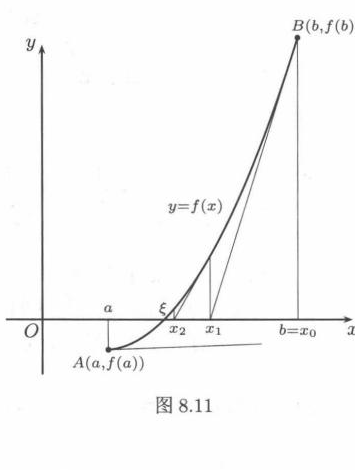
\includegraphics[width=.42\linewidth]{figures/upper/ch08/fig-8-11.png}
\end{center}

从图 8.11 可以看出，所得到的数列 $\{x_n\}$ 有可能会很快收敛到方程 $f(x)=0$ 的根 $\xi$。这就是 Newton 求根法，也称为 Newton 切线法。

但这里实际上有许多问题需要研究。首先，若设方程 $f(x)=0$ 在区间 $(a,b)$ 中只有唯一的一个根 $\xi$，是否一定成立
\[
  \lim_{n\to\infty}x_n=\xi.
\]
其次，这个算法的收敛速度如何？此外还有一个如何取初始值的问题。在图 8.11 上从点 $A(a,f(a))$ 也作出了曲线 $y=f(x)$ 的切线，但它与 $x$ 轴的交点（在图上未画出）很可能会越出函数 $f(x)$ 的定义域。

可以从完全不同的角度导出 Newton 求根法。例如，假定已得到根 $\xi$ 的第 $n$ 个近似值 $x_n$，又设 $f$ 二阶可微，则可以写出带 Lagrange 余项的 Taylor 展开式：
\begin{equation}
  0=f(\xi)=f(x_n)+f'(x_n)(\xi-x_n)+\frac{f''(\theta_n)}2(\xi-x_n)^2,
  \tag{8.28}
  \label{eq:8.28}
\end{equation}
其中的中值 $\theta_n$ 在 $x_n$ 和 $\xi$ 之间，在公式 (8.28) 中弃去右边的最后一项，并将由此得到的根 $\xi$ 的近似值记为 $x_{n+1}$，就得到了前面已有的公式 (8.27)。在将 Newton 求根法推广到高维空间时用这种局部线性化的方法没有本质上的困难。

现在给出保证 Newton 求根法能够成功的一组充分条件，并证明它的收敛速度恰好是二阶。为直观起见，下面所述的条件均与图 8.11 一致。读者可自行写出与这组充分条件平行的其他充分条件。

\begin{xtheorem}[8.7.1]
设函数 $f(x)$ 在区间 $[a,b]$ 上二阶连续可微，且满足以下条件：
\begin{enumerate}[label=(\arabic*)]
  \item $f(a)<0$，$f(b)>0$；
  \item $f'(x)>0$，$\forall x\in[a,b]$；
  \item $f''(x)>0$，$\forall x\in[a,b]$；
  \item 取 $x_0=b$ 为初始值；
\end{enumerate}
那么就有
\begin{enumerate}[label=(\arabic*)]
  \item 方程 $f(x)=0$ 在区间 $(a,b)$ 内存在唯一的根 $\xi$；
  \item 由递推公式 (8.27) 得到的数列 $\{x_n\}$ 是在区间 $[a,b]$ 中的严格单调减少数列，且以 $\xi$ 为极限；
  \item 数列 $\{x_n\}$ 的收敛速度为二阶。
\end{enumerate}
\end{xtheorem}
\begin{xproof}
从连续函数的零点存在定理知道方程 $f(x)=0$ 在 $(a,b)$ 中有根。从 $f'(x)$ 在区间上处处大于 0 可知函数 $f(x)$ 严格单调增加，因此方程的根唯一。

从公式 (8.28) 和 $f''(x)>0$，$\forall x\in[a,b]$ 可见，成立
\[
  f(x_n)+f'(x_n)(\xi-x_n)<0,\qquad\forall n\in\NN_+.
\]
由此即可得到
\[
  \xi<x_n-\frac{f(x_n)}{f'(x_n)}=x_{n+1},\qquad\forall n\in\NN_+.
\]
从递推公式 (8.27) 又可看出只要 $f(x_n)>0$，就有
\[
  x_{n+1}<x_n
\]
成立。由于初始值 $x_0=b$ 处有 $f(b)>0$，而当 $x_n>\xi$ 时就有 $f(x_n)>0$，因此就保证了数列 $\{x_n\}$ 是严格单调减少数列，且以 $\xi$ 为下界。记该数列的极限为 $\eta$，在公式 (8.27) 两边令 $n\to\infty$，得到
\[
  \eta=\eta-\frac{f(\eta)}{f'(\eta)},
\]
可见 $f(\eta)=0$。由于方程 $f(x)=0$ 在 $[a,b]$ 中的根唯一，因此 $\eta=\xi$。这样就证明了 Newton 求根法所得的迭代数列 $\{x_n\}$ 收敛于方程在区间 $[a,b]$ 中的唯一根。

现在用 Taylor 公式 (8.28) 估计迭代误差
\begin{align*}
  0<x_{n+1}-\xi
  &=x_n-\frac{f(x_n)}{f'(x_n)}-\xi\\
  &=\frac{(x_n-\xi)f'(x_n)-f(x_n)}{f'(x_n)}\\
  &=\frac{f''(\theta_n)(x_n-\xi)^2}{2f'(x_n)},
\end{align*}
其中 $\theta_n\in(\xi,x_n)$。利用 $f''$ 连续且处处大于 0，就有
\[
  \lim_{n\to\infty}\frac{x_{n+1}-\xi}{(x_n-\xi)^2}
  =\frac{f''(\xi)}{2f'(\xi)}\ne0.
\]
因此 $\{x_n\}$ 二阶收敛于 $\xi$。
\end{xproof}

\begin{xremark}
\textbf{注 1}\quad 容易看到在命题中的某些条件可以放宽，而仍保证迭代数列为二阶收敛或不低于二阶收敛。但另一方面也可以举出各种例子，说明在 4 个条件中的某些条件不成立时，Newton 求根法可能失败。一般而言，Newton 求根法在有拐点、重根和多根时会有困难。

\textbf{注 2}\quad 不难得到 Newton 求根法的先验估计和事后估计（可以与命题 3.4.4，即压缩映射原理中的结果作比较）。由于 $f$ 在 $[a,b]$ 上二阶连续可微，因此在命题的条件下 $f''$ 在 $[a,b]$ 上有最大值 $M>0$，而 $f'(x)$ 在 $[a,b]$ 上有最小值 $m=f'(a)>0$。从证明中关于迭代误差的估计有
\[
  |x_{n+1}-\xi|\le\frac{M}{2m}|x_n-\xi|^2,
\]
代入公式 (8.25) 就得到
\[
  |x_n-\xi|\le\frac{2m}{M}
  \left(\frac{M}{2m}|x_0-\xi|\right)^{2^n}.
\]
在计算前，用它可以估计为达到指定精度所需的迭代次数，即先验估计。

注意：为了满足 $\dfrac{M}{2m}|x_0-\xi|<1$ 的要求，区间 $[a,b]$ 的长度应当满足不等式
\[
  b-a<\frac{2m}{M}.
\]
但从命题的证明知道，即使这个条件不成立，迭代数列仍然二阶收敛。

再利用 Lagrange 中值定理得到
\[
  |f(x_n)-f(\xi)|=|f(x_n)|\ge m|x_n-\xi|,
\]
又用 Taylor 公式有
\begin{align*}
  f(x_n)
  &=f(x_{n-1})+f'(x_{n-1})(x_n-x_{n-1})
    +\frac{f''(\eta)}2(x_n-x_{n-1})^2\\
  &=\frac{f''(\eta)}2(x_n-x_{n-1})^2,
\end{align*}
其中 $\eta$ 在 $x_n$ 与 $x_{n-1}$ 之间，就可以得到
\[
  |x_n-\xi|\le\frac1m|f(x_n)|
  \le\frac{M}{2m}|x_n-x_{n-1}|^2.
\]
这可用于从相继两次计算的结果去估计当时的误差大小，即事后估计。
\end{xremark}

\begin{xexample}[8.7.4]
用 Newton 求根法导出开平方根的迭代算法。
\end{xexample}
\begin{xsolution}
设要求正数 $A$ 的平方根。取函数 $f(x)=x^2-A$，求 $\sqrt A$ 的问题就成为方程求根问题了。将 $f$ 代入迭代公式 (8.27) 中，就得到
\[
  x_{n+1}=x_n-\frac{x_n^2-A}{2x_n}
  =\frac{x_n}{2}+\frac{A}{2x_n}.
\]
\end{xsolution}

\begin{xremark}
\textbf{注 1}\quad 在 $A=2$ 时就得到例题 8.7.3 中的算法。实际上本题的算法已在 2.6.3 小节的练习题 8 中出现。其中练习题 9 还给出了求平方根的一个三阶算法。

\textbf{注 2}\quad 这个算法的历史可以上溯到古代巴比伦文明（见 [35]）。其思路可能是：如果 $x$ 是 $\sqrt A$ 的一个近似值，那么 $A/x$ 也是一个近似值，这两个近似值的乘积等于 $A$，而且分别在 $\sqrt A$ 的两侧，因此取算术平均值可能会得到更好的结果。
\end{xremark}

\subsection{练习题}

本节的计算题应当根据在学习中所能使用的计算工具来安排，下面的题中只有第 1 题是计算题，且只需用计算器。

\begin{xexercise}[1]
用 Newton 求根法计算（要求精确到 $0.0001$）：
  \begin{enumerate}[label=(\arabic*)]
    \item $x^3-2x^2-4x-7=0$ 在 $[3,4]$ 之间的根的近似值；
    \item $\sin x=1-x$ 的根的近似值。
  \end{enumerate}
\end{xexercise}
\begin{xsolution}
\begin{enumerate}[label=(\arabic*)]
  \item 对
  \[
    f(x)=x^3-2x^2-4x-7
  \]
  用 Newton 迭代
  \[
    x_{n+1}=x_n-\frac{x_n^3-2x_n^2-4x_n-7}{3x_n^2-4x_n-4}.
  \]
  取 $x_0=4$，依次得到
  \[
    4,\ 3.67857143,\ 3.63287255,\ 3.63198114,\ 3.63198081,\ldots
  \]
  因而精确到 $0.0001$ 的根为
  \[
    \boxed{3.6320}.
  \]

  \item 写成 $f(x)=\sin x+x-1=0$，Newton 迭代为
  \[
    x_{n+1}=x_n-\frac{\sin x_n+x_n-1}{\cos x_n+1}.
  \]
  取 $x_0=0.5$，得到
  \[
    0.5,\ 0.51095795,\ 0.51097343,\ldots
  \]
  故根的近似值为
  \[
    \boxed{0.5110}.
  \]
\end{enumerate}
\end{xsolution}


\begin{xexercise}[2]
在命题 8.7.1 中给出了保证 Newton 求根法成功的充分条件，其中共有 4 项要求。试举出例子，说明不满足其中的某些要求时，用 Newton 求根法有可能失败。
\end{xexercise}
\begin{xsolution}
以下例子说明命题中的条件确实不能任意删去。

若导数在初值处为零，例如用 Newton 法解
\[
  f(x)=x^3-1=0,
\]
却取 $x_0=0$，则第一步就因 $f'(0)=0$ 而无法定义。

即使每一步都能定义，也可能不收敛。例如
\[
  f(x)=x^3-2x+2,\qquad x_0=0.
\]
Newton 映射为
\[
  N(x)=x-\frac{x^3-2x+2}{3x^2-2}.
\]
直接算得
\[
  N(0)=1,\qquad N(1)=0,
\]
故迭代在 $0,1$ 之间形成二周期而失败。这说明没有合适的单调性、凸性与初值控制时，即使方程有实根，Newton 法也可能不收敛到根。
\end{xsolution}


\begin{xexercise}[3]
证明：在例题 5.2.1 中提供的二分法是方程求根的一阶算法。
\end{xexercise}
\begin{xsolution}
二分法每一步把当前含根区间的长度减半。若以区间半长作为误差上界 $\varepsilon_n$，则
\[
  \varepsilon_{n+1}=\frac12\varepsilon_n.
\]
因此
\[
  \lim_{n\to\infty}\frac{\varepsilon_{n+1}}{\varepsilon_n}=\frac12\ne0,
\]
按本节定义二分法是一阶算法。
\end{xsolution}


\begin{xexercise}[4]
证明：2.6.3 小节的题 9 中的算法是求平方根的三阶算法。
\end{xexercise}
\begin{xsolution}
题 9 中求 $\sqrt A$ 的迭代式为
\[
  x_{n+1}=\frac{x_n(x_n^2+3A)}{3x_n^2+A},
  \qquad A>0,\quad x_0>0.
\]
令 $r=\sqrt A$，$t_n=x_n/r$，则
\[
  t_{n+1}=T(t_n),
  \qquad
  T(t)=\frac{t(t^2+3)}{3t^2+1}.
\]
直接计算得
\[
  T(t)-1=\frac{(t-1)^3}{3t^2+1},
  \qquad
  T(t)-t=\frac{2t(1-t^2)}{3t^2+1}.
\]
故当 $t>1$ 时 $1<T(t)<t$，当 $0<t<1$ 时 $t<T(t)<1$。因此 $\{t_n\}$ 单调有界并收敛，其极限只能为 $1$，即 $x_n\to r$。

更重要的是有精确误差关系
\[
  x_{n+1}-r
  =\frac{(x_n-r)^3}{3x_n^2+A}.
\]
于是
\[
  \lim_{n\to\infty}
  \frac{x_{n+1}-r}{(x_n-r)^3}
  =\frac1{3r^2+A}
  =\frac1{4A}\ne0.
\]
所以该算法为求平方根的三阶收敛算法。
\end{xsolution}


\begin{xexercise}[5]
设 $A>0$，为计算立方根 $\sqrt[3]A$，从 $x_0>0$ 出发用递推公式
  \[
    x_{n+1}=\frac{x_n(x_n^3+2A)}{2x_n^3+A}
  \]
  作迭代，证明数列 $\{x_n\}$ 收敛，求出其极限，并确定其收敛的阶。
\end{xexercise}
\begin{xsolution}
令 $r=\sqrt[3]A>0$，并设 $t_n=x_n/r$。递推式化为
\[
  t_{n+1}=T(t_n),
  \qquad
  T(t)=\frac{t(t^3+2)}{2t^3+1}.
\]
直接因式分解：
\[
  T(t)-1=\frac{(t-1)^3(t+1)}{2t^3+1},
  \qquad
  T(t)-t=\frac{t(1-t^3)}{2t^3+1}.
\]
因此若 $t>1$，则 $1<T(t)<t$；若 $0<t<1$，则 $t<T(t)<1$。故从任意 $t_0>0$ 出发，数列单调有界并收敛，极限只能是 $1$。所以
\[
  \boxed{x_n\to r=\sqrt[3]A}.
\]

再令 $e_n=x_n-r$。由上面的精确因式分解，
\[
  e_{n+1}
  =r\frac{(e_n/r)^3(2+e_n/r)}{2(1+e_n/r)^3+1},
\]
故
\[
  \lim_{n\to\infty}\frac{e_{n+1}}{e_n^3}
  =\frac{2}{3r^2}\ne0.
\]
所以该算法为三阶收敛。
\end{xsolution}


\begin{xexercise}[6]
用 Newton 求根法设计一个求 $\sqrt[k]A$（$A>0,k>0$）的迭代算法，并对其收敛速度作出分析。
\end{xexercise}
\begin{xsolution}
取
\[
  f(x)=x^k-A,
\]
Newton 公式给出
\[
  \boxed{x_{n+1}
  =x_n-\frac{x_n^k-A}{kx_n^{k-1}}
  =\frac1k\left((k-1)x_n+\frac{A}{x_n^{k-1}}\right)}.
\]
这里按通常实数 $k$ 次根问题取 $k>1$；$k=1$ 时一步即得精确值。令 $r=A^{1/k}$，$e_n=x_n-r$。Newton 法的标准 Taylor 误差式给出
\[
  e_{n+1}
  =\frac{f''(r)}{2f'(r)}e_n^2+\littleo(e_n^2)
  =\frac{k-1}{2r}e_n^2+\littleo(e_n^2).
\]
故当初值取在 $r$ 的充分小正邻域内时迭代收敛，且收敛阶为二阶。
\end{xsolution}


\begin{xexercise}[7]
用 Newton 求根法设计一个求 $1/A$ 的迭代算法，其中只用加法和乘法运算，并对其收敛速度作出分析。
\end{xexercise}
\begin{xsolution}
要求 $1/A$，对方程
\[
  f(x)=\frac1x-A=0
\]
应用 Newton 法：
\[
  x_{n+1}
  =x_n-\frac{1/x_n-A}{-1/x_n^2}
  =\boxed{x_n(2-Ax_n)}.
\]
这个公式只含加法与乘法。

令
\[
  \delta_n=1-Ax_n.
\]
则有精确递推关系
\[
  \delta_{n+1}=\delta_n^2.
\]
若初值满足 $0<Ax_0<2$，即 $|\delta_0|<1$，则 $\delta_n\to0$，故 $x_n\to1/A$。又令 $e_n=x_n-1/A$，则
\[
  e_{n+1}=-A e_n^2,
\]
因此收敛恰为二阶。
\end{xsolution}


\section{对于教学的建议}

微分学的应用极其广泛，本章只介绍了其中的一部分内容，主要是对于函数的研究，还包括极限计算与方程求根的近似计算方法。其他如曲率、渐屈线与渐伸线等在几何学上的应用均未收入。有需要的读者可以从 [14, 8, 27, 59, 72] 等文献中找到微分学应用方面的更多材料。

\subsection{学习要点}

1. L'Hospital 法则无疑是求函数极限的首选工具。但是若使用不当则会带来复杂的计算。如何能综合使用包括 Taylor 公式在内的各种方法，初学者需要通过大量的训练才能掌握。今后学了积分学和无穷级数等知识后，还会提供计算极限的许多新工具，因此计算极限这一主题并非到此为止。复习考研的学生尤其要注意这一点。

2. 函数的单调性分析（即确定其单调区间）以及函数极值和最值的确定，这些都是函数研究中的基本问题。这方面可以参考 [27, 59] 的 §2.7，§2.11。对具有实际背景的极值应用问题感兴趣的读者，可以从 [27, 59] 的 §2.13 得到丰富多彩的材料（例题 8.3.4 即是 [27] 中的习题 1587）。

3. 凸函数在数学中是一类很重要的函数，在理论和应用上均有其独特的地位。有关凸函数的考题在考研中也是常见的。本章对凸函数和有关的不等式作了基本的介绍。请读者注意其中每个结论均有明显的几何意义，由此出发不难掌握有关的结论和证明。此外，在凸函数中的许多有关问题可以从不用导数、利用一阶导数和利用二阶导数三个层次来进行研究。一个典型例子就是在本书中出现多次的 Jensen 不等式（即命题 8.4.7）。

4. 不等式在几乎每个数学领域中都是一个重要主题。可以看出，与本书第一章 §1.3 的初等不等式相比，在本章中我们对不等式的认识上升到了一个全新的水平。事实上在今后，随着数学分析（以及其他课程）的学习，不等式会一再出现，在内容和方法上都会有层出不穷的新东西。例如在 8.5.2 小节中的三个经典不等式在积分学和无穷级数中就都会遇到，这方面的内容极其丰富。§8.5 是用微分学来研究不等式，在后面的 §11.2 则是用积分学来研究不等式。应当指出，[30] 是我国学者所写的不等式方面的专著，材料极其丰富，很有参考价值。

5. 微分学在函数作图方面的应用是明显的。但是应当看到，除了用微分学的作图方法之外，还存在另外一种作草图的简便方法。这就是利用曲线的“四则运算”和移位、按比例放大缩小等技巧，将曲线的大致趋势迅速确定出来。值得注意的是在部分教科书中还专门介绍了这个方法（例如见 [42, 72]）。在经典习题集 [27] 中为此将这两种不同的作图方法的练习分别安排在 §1.4 和 §2.12 中。希望上习题课的教师注意不要漏掉这方面的训练。在 [59] 的 §1.4 和 §2.12 有很多详细解答的例题可供参考。

6. 近似计算问题应当在数学分析的教学中占有一定的分量。尽早培养学生在这方面的意识是数学分析在今后的改革方向之一。从第二章开始，本书注意了介绍这方面的内容。当然这里还有许多不足之处。若有可能，希望在数学分析的教学中加入简单编程计算和使用 Mathematica 等软件的内容。实际上本书的部分例题就是用 Mathematica 来计算的（例如例题 8.7.3）。

7. \textbf{对习题课的建议}\quad 本章习题课的材料很丰富，都比较具体。需要注意的是不要在习题课上草草过场，对有关材料要充分展开。通过应用微分学解决实际问题，让学生加强应用的意识，提高应用的能力。凸函数、不等式都是很重要的题材，需要在习题课上专门花时间训练。

\subsection{参考题}

\paragraph{第一组参考题}

\begin{xreferenceproblem}[1]
\begin{enumerate}[label=(\arabic*)]
    \item 设 $\displaystyle\lim_{x\to+\infty}[f(x)+f'(x)]=0$，证明：$\displaystyle\lim_{x\to+\infty}f(x)=0$；
    \item 设 $|f(x)+f'(x)|\le1$，$f(x)$ 在 $(-\infty,+\infty)$ 上有界，证明：$|f(x)|\le1$。
  \end{enumerate}
\end{xreferenceproblem}
\begin{xsolution}
\begin{enumerate}[label=(\arabic*)]
  \item 记 $h(x)=f(x)+f'(x)$。给定 $\varepsilon>0$，存在 $X$，当 $x\ge X$ 时 $|h(x)|<\varepsilon$。于是
  \[
    [\ee^x(f(x)-\varepsilon)]'
    =\ee^x(h(x)-\varepsilon)<0,
  \]
  \[
    [\ee^x(f(x)+\varepsilon)]'
    =\ee^x(h(x)+\varepsilon)>0.
  \]
  对 $x\ge X$ 积分意义等价的单调性比较给出
  \[
    -\varepsilon+C_1\ee^{-x}\le f(x)
    \le\varepsilon+C_2\ee^{-x},
  \]
  其中常数由 $X$ 处的值决定。令 $x\to+\infty$，得
  \[
    -\varepsilon\le\liminf f(x)\le\limsup f(x)\le\varepsilon.
  \]
  再令 $\varepsilon\downarrow0$，即得 $f(x)\to0$。

  \item 设反面存在 $x_0$ 使 $f(x_0)>1$。由
  \[
    f+f'\le1
  \]
  得 $\ee^x(f-1)$ 单调不增。因此对 $x<x_0$，
  \[
    f(x)-1\ge\ee^{x_0-x}[f(x_0)-1]\to+\infty
    \quad(x\to-\infty),
  \]
  与 $f$ 有界矛盾。若存在 $f(x_0)<-1$，由 $f+f'\ge-1$ 知 $\ee^x(f+1)$ 单调不减，于 $x<x_0$ 得 $f(x)\to-\infty$，同样矛盾。故
  \[
    |f(x)|\le1\qquad(\forall x\in\RR).
  \]
\end{enumerate}
\end{xsolution}


\begin{xreferenceproblem}[2]
设 $f(x)$ 在 $x=0$ 的某邻域上二阶可微，且
  \[
    \lim_{x\to0}\left(1+x+\frac{f(x)}x\right)^{1/x}=\ee^3.
  \]
  求 $f(0)$，$f'(0)$，$f''(0)$ 和
  \[
    \lim_{x\to0}\left(1+\frac{f(x)}x\right)^{1/x}.
  \]
\end{xreferenceproblem}
\begin{xsolution}
由题设
\[
  \frac1x\ln\left(1+x+\frac{f(x)}x\right)\to3.
\]
有限两侧极限迫使括号趋于 1。若 $f(0)\ne0$，则 $f(x)/x$ 无界，不可能成立，故 $f(0)=0$。写 Taylor 展开
\[
  f(x)=f'(0)x+\frac12f''(0)x^2+\littleo(x^2).
\]
于是括号的极限为 $1+f'(0)$，故还必须有 $f'(0)=0$。此时
\[
  1+x+\frac{f(x)}x
  =1+\left(1+\frac12f''(0)\right)x+\littleo(x).
\]
因此
\[
  3=1+\frac12f''(0),
  \qquad f''(0)=4.
\]
最后
\[
  1+\frac{f(x)}x=1+2x+\littleo(x),
\]
故
\[
  \boxed{f(0)=0,\quad f'(0)=0,\quad f''(0)=4,\quad
  \lim_{x\to0}\left(1+\frac{f(x)}x\right)^{1/x}=\ee^2}.
\]
\end{xsolution}


\begin{xreferenceproblem}[3]
例题 8.1.10 可以推广如下：设正数列 $\{x_n\}$ 为满足递推公式 $x_{n+1}=f(x_n)$ 的无穷小量，函数 $f$ 有 Maclaurin 展开式
  \[
    f(x)=x+Ax^k+\littleo(x^k)\quad(x\to0),
  \]
  其中 $k$ 为大于 1 的某正整数，系数 $A\ne0$，证明：有 $\alpha>0$，使得存在非零极限 $\displaystyle\lim_{n\to\infty}nx_n^\alpha$，并求出此极限。
\end{xreferenceproblem}
\begin{xsolution}
由正数列 $x_n\to0$ 且
\[
  x_{n+1}=x_n+Ax_n^k+\littleo(x_n^k),
\]
必有 $A<0$；否则在充分大的 $n$ 上 $x_{n+1}>x_n$，与正数列趋于 0 矛盾。

令
\[
  y_n=x_n^{-(k-1)}\to+\infty.
\]
则
\begin{align*}
  y_{n+1}-y_n
  &=x_n^{-(k-1)}
  \left[
    \left(1+Ax_n^{k-1}+\littleo(x_n^{k-1})\right)^{-(k-1)}-1
  \right]\\
  &\to-(k-1)A>0.
\end{align*}
由 Stolz 定理，
\[
  \frac{y_n}{n}\to-(k-1)A.
\]
因此应取
\[
  \boxed{\alpha=k-1},
\]
且
\[
  \boxed{\lim_{n\to\infty}n x_n^{k-1}
  =-\frac1{(k-1)A}>0}.
\]
\end{xsolution}


\begin{xreferenceproblem}[4]
设 $f\in C[a,b]$，证明：$f$ 在 $(a,b)$ 内没有极值点的充分必要条件是 $f$ 在区间 $[a,b]$ 上为严格单调函数。
\end{xreferenceproblem}
\begin{xsolution}
严格单调函数显然没有内点极值。

反之，设 $f$ 在 $(a,b)$ 内没有极值点。先证 $f$ 为一一函数。若存在 $x<y$ 使 $f(x)=f(y)$，则连续函数在 $[x,y]$ 上取得最大、最小值。若 $f$ 在该区间恒定，则任一内点都是极值点；若不恒定，则最大值或最小值中至少有一个与端点公共值不同，从而必在 $(x,y)$ 内取得，仍产生极值点。均矛盾。因此 $f$ 一一。

连续的一一实函数在区间上必严格单调，故 $f$ 在 $[a,b]$ 上严格单调。
\end{xsolution}


\begin{xreferenceproblem}[5]
证明关于三点不等式（命题 1.3.4）的一个推广：在 $0<p<1$ 时，成立不等式
  \[
    |a+b|^p\le|a|^p+|b|^p.
  \]
\end{xreferenceproblem}
\begin{xsolution}
只需证明对 $u,v\ge0$，
\[
  (u+v)^p\le u^p+v^p,
  \qquad0<p<1.
\]
若 $u=0$ 或 $v=0$ 显然。设 $u>0$，令 $t=v/u\ge0$，只需证
\[
  (1+t)^p\le1+t^p.
\]
令 $F(t)=1+t^p-(1+t)^p$，则 $F(0)=0$，且
\[
  F'(t)=p[t^{p-1}-(1+t)^{p-1}]>0
\]
因为 $p-1<0$。故 $F(t)\ge0$。取 $u=|a|$、$v=|b|$，再用三角不等式，
\[
  |a+b|^p\le(|a|+|b|)^p\le|a|^p+|b|^p.
\]
\end{xsolution}


\begin{xreferenceproblem}[6]
证明：对每个正整数 $n$，成立不等式
  \[
    \frac{\ee}{2n+2}<\ee-\left(1+\frac1n\right)^n<\frac{\ee}{2n+1}.
  \]
\end{xreferenceproblem}
\begin{xsolution}
令 $t=1/n>0$，并记
\[
  r=1-\frac{\ln(1+t)}t>0.
\]
则
\[
  \frac1\ee\left[\ee-(1+t)^{1/t}\right]=1-\ee^{-r}.
\]
先证上界。由 $1-\ee^{-r}<r$ 以及例题 8.5.1 的强化式
\[
  \ln(1+t)>\frac{2t}{2+t}
\]
得
\[
  r<\frac{t}{2+t},
\]
所以
\[
  1-\ee^{-r}<\frac{t}{2+t}=\frac1{2n+1}.
\]

再证下界。要证
\[
  1-\ee^{-r}>\frac{t}{2(1+t)},
\]
等价于
\[
  r>\ln\frac{1+t}{1+t/2}.
\]
令
\[
  H(t)=1+\ln(1+t/2)-\left(1+\frac1t\right)\ln(1+t).
\]
有 $H(0+)=0$，并且
\[
  H'(t)=\frac{(t+2)\ln(1+t)-2t}{t^2(t+2)}>0,
\]
最后一步仍由 $\ln(1+t)>2t/(2+t)$。故 $H(t)>0$，下界成立。恢复 $t=1/n$，得到
\[
  \boxed{
  \frac{\ee}{2n+2}<\ee-\left(1+\frac1n\right)^n
  <\frac{\ee}{2n+1}}.
\]
\end{xsolution}


\begin{xreferenceproblem}[7]
证明：当 $0<x<\dfrac\pi2$ 时，成立不等式
  \[
    \left(\frac{\sin x}{x}\right)^3>\cos x.
  \]
\end{xreferenceproblem}
\begin{xsolution}
令
\[
  F(x)=3\ln\frac{\sin x}{x}-\ln\cos x,
  \qquad0<x<\frac\pi2.
\]
有 $F(0+)=0$。化简导数：
\[
  F'(x)=
  \frac{x(1+2\cos^2x)-3\sin x\cos x}{x\sin x\cos x}.
\]
记分子为 $N(x)$。则 $N(0)=0$，且
\[
  N'(x)=4\sin x(\sin x-x\cos x).
\]
而 $G(x)=\sin x-x\cos x$ 满足 $G(0)=0$、$G'(x)=x\sin x>0$，故 $G(x)>0$，从而 $N'(x)>0$。所以 $F'(x)>0$、$F(x)>0$。指数化即得
\[
  \left(\frac{\sin x}{x}\right)^3>\cos x.
\]
\end{xsolution}


\begin{xreferenceproblem}[8]
证明：当 $0<x<\dfrac\pi2$ 时，成立不等式 $2\sin x+\tan x>3x$。
\end{xreferenceproblem}
\begin{xsolution}
令
\[
  F(x)=2\sin x+\tan x-3x.
\]
则 $F(0)=0$，且
\begin{align*}
  F'(x)
  &=2\cos x+\operatorname{sec}^2x-3\\
  &=\frac{(1-\cos x)^2(2\cos x+1)}{\cos^2x}>0
\end{align*}
对 $0<x<\pi/2$ 成立。因此 $F(x)>0$，即所证不等式。
\end{xsolution}


\begin{xreferenceproblem}[9]
证明：当 $0<x<1$ 时，成立不等式
  \[
    \pi<\frac{\sin\pi x}{x(1-x)}\le4.
  \]
\end{xreferenceproblem}
\begin{xsolution}
先证下界。令
\[
  h(x)=\sin\pi x-\pi x(1-x).
\]
函数关于 $x=1/2$ 对称，只需看 $0<x<1/2$。此时
\[
  h'(x)=\pi[\cos\pi x-1+2x].
\]
因 $\cos t$ 在 $[0,\pi/2]$ 上严格上凸，图像严格高于连接端点的弦
\[
  \cos t>1-\frac{2t}{\pi},
\]
故 $h'(x)>0$，于是 $h(x)>h(0)=0$，即
\[
  \frac{\sin\pi x}{x(1-x)}>\pi.
\]

再证上界，令
\[
  H(x)=4x(1-x)-\sin\pi x.
\]
仍只需看 $[0,1/2]$。有 $H(0)=H(1/2)=0$，
\[
  H'=4-8x-\pi\cos\pi x,
  \quad H''=-8+\pi^2\sin\pi x,
  \quad H'''=\pi^3\cos\pi x>0.
\]
故 $H''$ 严格增加并只变号一次，$H'$ 先减后增；结合 $H'(0)=4-\pi>0$、$H'(1/2)=0$ 以及 $H(1/2)-H(0)=0$，可知 $H'$ 在内部只从正变负一次，故 $H$ 先增后减并保持非负。于是
\[
  \sin\pi x\le4x(1-x).
\]
等号在 $x=1/2$ 成立。综上即得题中双边不等式。
\end{xsolution}


\begin{xreferenceproblem}[10]
证明：当 $x\in[0,\pi/2]$ 时，成立比 Jordan 不等式（例题 8.5.6）更好的结果：
  \[
    \sin x\ge\frac2\pi x+\frac1{12\pi}x(\pi^2-4x^2).
  \]
\end{xreferenceproblem}
\begin{xsolution}
记
\[
  F(x)=\sin x-\frac2\pi x-\frac1{12\pi}x(\pi^2-4x^2).
\]
直接验证 $F(0)=F(\pi/2)=0$，而
\[
  F''(x)=\frac{2x}{\pi}-\sin x\le0
\]
由 Jordan 不等式成立。因此 $F$ 在 $[0,\pi/2]$ 上为上凸函数。上凸函数的图像在连接两个端点的弦之上，而该弦就是 $y=0$，故 $F(x)\ge0$，即得所证强化不等式。
\end{xsolution}


\begin{xreferenceproblem}[11]
证明：对 $n$ 个正数 $x_1,x_2,\ldots,x_n$，成立不等式
  \[
    \frac{x_1x_2\cdots x_n}{(x_1+x_2+\cdots+x_n)^n}
    \le
    \frac{(1+x_1)(1+x_2)\cdots(1+x_n)}{(n+x_1+x_2+\cdots+x_n)^n},
  \]
  并讨论成立等号的条件。
\end{xreferenceproblem}
\begin{xsolution}
记
\[
  S=x_1+\cdots+x_n,
  \quad y_i=\frac{x_i}{S},
  \quad z_i=\frac{1+x_i}{n+S}.
\]
则 $\sum y_i=\sum z_i=1$，且
\[
  z_i=\frac{S}{n+S}y_i+\frac{n}{n+S}\frac1n.
\]
由于 $\ln$ 为上凸函数，
\[
  \sum\ln z_i
  \ge\frac{S}{n+S}\sum\ln y_i
   +\frac{n}{n+S}\,n\ln\frac1n.
\]
而 AM--GM 给出
\[
  \sum\ln y_i\le n\ln\frac1n.
\]
因此右端不小于 $\sum\ln y_i$，从而
\[
  \prod z_i\ge\prod y_i.
\]
展开定义正是题中不等式。两处等号同时成立当且仅当
\[
  x_1=x_2=\cdots=x_n.
\]
\end{xsolution}


\begin{xreferenceproblem}[12]
证明：当 $x\in(0,\pi/4)$ 时，成立 $(\sin x)^{\cos x}<(\cos x)^{\sin x}$；而在 $x\in(\pi/4,\pi/2)$ 时，不等式反向。
\end{xreferenceproblem}
\begin{xsolution}
两边取对数。所需比较等价于
\[
  \frac{\ln\sin x}{\sin x}
  \quad\text{与}\quad
  \frac{\ln\cos x}{\cos x}
\]
的大小。令
\[
  \phi(t)=\frac{\ln t}{t},\qquad0<t\le1.
\]
则
\[
  \phi'(t)=\frac{1-\ln t}{t^2}>0,
\]
所以 $\phi$ 严格增加。当 $0<x<\pi/4$ 时 $\sin x<\cos x$，故
\[
  \frac{\ln\sin x}{\sin x}<\frac{\ln\cos x}{\cos x},
\]
等价于 $(\sin x)^{\cos x}<(\cos x)^{\sin x}$。当 $\pi/4<x<\pi/2$ 时次序反向，故不等式也反向。
\end{xsolution}


\begin{xreferenceproblem}[13]
设 $p>1$，$a,b>0$，证明：
  \begin{enumerate}[label=(\arabic*)]
    \item 当 $t>0$ 时，成立
    \[
      \frac1p t^{1/p-1}a+\left(1-\frac1p\right)t^{1/p}b
      \ge a^{1/p}b^{1-1/p};
    \]
    \item 当 $0<t<1$ 时，成立
    \[
      t^{1-p}a^p+(1-t)^{1-p}b^p\ge(a+b)^p.
    \]
  \end{enumerate}
\end{xreferenceproblem}
\begin{xsolution}
\begin{enumerate}[label=(\arabic*)]
  \item 对两个正数
  \[
    X=t^{1/p-1}a,
    \qquad Y=t^{1/p}b
  \]
  应用权分别为 $1/p$ 和 $1-1/p$ 的加权 AM--GM：
  \[
    \frac Xp+\left(1-\frac1p\right)Y
    \ge X^{1/p}Y^{1-1/p}.
  \]
  右端的 $t$ 次幂恰相消，故得到题中 (1)。

  \item 令
  \[
    F(t)=\frac{a^p}{t^{p-1}}+
          \frac{b^p}{(1-t)^{p-1}},\qquad0<t<1.
  \]
  有
  \[
    F'(t)=-(p-1)\frac{a^p}{t^p}
    +(p-1)\frac{b^p}{(1-t)^p}.
  \]
  唯一驻点为 $t=a/(a+b)$，且 $F$ 在其左侧减少、右侧增加，所以该点为全局最小值点。代入得到
  \[
    F_{\min}=(a+b)^p.
  \]
  这就是题中 (2)。
\end{enumerate}
\end{xsolution}


\begin{xreferenceproblem}[14]
设 $p(x)$ 为三次多项式，$p(a)=p(b)=0$，证明：$p(x)$ 在 $[a,b]$ 上不变号的充分必要条件是 $p'(a)p'(b)\le0$。
\end{xreferenceproblem}
\begin{xsolution}
写成
\[
  p(x)=C(x-a)(x-b)(x-c),\qquad C\ne0,
\]
其中第三个根 $c$ 为实数。$p$ 在 $[a,b]$ 上不变号，当且仅当第三个根不在开区间 $(a,b)$ 中，即
\[
  (a-c)(b-c)\ge0.
\]
另一方面
\[
  p'(a)p'(b)
  =-C^2(a-b)^2(a-c)(b-c).
\]
故
\[
  p'(a)p'(b)\le0
  \quad\Longleftrightarrow\quad
  (a-c)(b-c)\ge0,
\]
恰与不变号条件等价。
\end{xsolution}


\begin{xreferenceproblem}[15]
证明在 $\RR$ 上的任何可微函数都不可能满足下列函数方程：
  \begin{enumerate}[label=(\arabic*)]
    \item $g(g(x))=-x^3+x+1$；
    \item $g(g(x))=-x^3+x^2+1$；
    \item $g(g(x))=x^2-3x+3$。
  \end{enumerate}
\end{xreferenceproblem}
\begin{xsolution}
设右端多项式统一记为 $P$。若 $P=g\circ g$，则必有交换关系
\[
  g(P(x))=P(g(x)).
\]
因此 $g$ 把 $P$ 的不动点映到 $P$ 的不动点。
\begin{enumerate}[label=(\arabic*)]
  \item $P(x)=-x^3+x+1$ 的唯一不动点为 $1$。故 $g(1)=1$。链式法则给出
  \[
    P'(1)=[g'(1)]^2\ge0,
  \]
  但 $P'(1)=-2$，矛盾。

  \item $P(x)=-x^3+x^2+1$ 的唯一不动点仍为 $1$，同理应有 $P'(1)=[g'(1)]^2\ge0$，但 $P'(1)=-1$，矛盾。

  \item $P(x)=x^2-3x+3$ 的不动点为 $1,3$。若 $g(1)=1$，则 $P'(1)=[g'(1)]^2\ge0$，但 $P'(1)=-1$，矛盾。因此 $g(1)=3$，又由 $g(g(1))=P(1)=1$ 得 $g(3)=1$。于是
  \[
    P'(1)=g'(3)g'(1)=P'(3),
  \]
  但 $P'(1)=-1$、$P'(3)=3$，矛盾。
\end{enumerate}
故三式均不存在全实轴可微解。
\end{xsolution}


\begin{xreferenceproblem}[16]
设 $f$ 在 $[0,1]$ 上二阶可微，$f(0)=f(1)=0$，$\displaystyle\min_{0\le x\le1}\{f(x)\}=-1$，证明：存在 $\xi\in(0,1)$，使成立 $f''(\xi)\ge8$。
\end{xreferenceproblem}
\begin{xsolution}
因端点值均为 0 而最小值为 $-1$，存在 $c\in(0,1)$ 使
\[
  f(c)=-1,\qquad f'(c)=0.
\]
对区间 $[0,c]$ 在 $c$ 点作二阶 Taylor 公式，存在 $\xi_1\in(0,c)$ 使
\[
  0=f(0)=f(c)+\frac12f''(\xi_1)c^2,
\]
故
\[
  f''(\xi_1)=\frac2{c^2}.
\]
同理存在 $\xi_2\in(c,1)$ 使
\[
  f''(\xi_2)=\frac2{(1-c)^2}.
\]
$c$ 与 $1-c$ 至少一个不超过 $1/2$，所以相应的二阶导数至少为 8。故存在所需 $\xi$。
\end{xsolution}


\begin{xreferenceproblem}[17]
设 $f$ 在 $[-1,1]$ 上二阶可微，$f(0)=f'(0)=0$，$f(1)=1$，$f(-1)=0$，证明：存在 $\xi\in(-1,1)$，使成立 $f''(\xi)=3$。
\end{xreferenceproblem}
\begin{xsolution}
原题按所印条件不能成立。取
\[
  f(x)=
  \begin{cases}
    x^2+x^3,&-1\le x\le0,\\
    x^2,&0\le x\le1.
  \end{cases}
\]
则两侧在 $0$ 处的一、二阶导数均接合，故 $f$ 在 $[-1,1]$ 上二阶可微，并且
\[
  f(0)=f'(0)=0,\qquad f(1)=1,\qquad f(-1)=0.
\]
但
\[
  f''(x)=
  \begin{cases}
    2+6x,&x<0,\\
    2,&x\ge0,
  \end{cases}
\]
在 $(-1,1)$ 内从不取值 3。因此题面所述结论为假。
\end{xsolution}


\begin{xreferenceproblem}[18]
设 $f,g$ 在 $[a,b]$ 上连续可微，$f(a)=f(b)=0$，Wronski（朗斯基）行列式
  \[
    W(f,g)=
    \begin{vmatrix}
      f(x)&g(x)\\
      f'(x)&g'(x)
    \end{vmatrix}
    \ne0,\qquad\forall x\in[a,b],
  \]
  证明：$g(x)$ 在 $(a,b)$ 中有零点。
\end{xreferenceproblem}
\begin{xsolution}
反设 $g$ 在 $(a,b)$ 内无零点。先看端点：由 $f(a)=0$ 与 $W(f,g)(a)\ne0$，
\[
  W(f,g)(a)=-g(a)f'(a)\ne0,
\]
所以 $g(a)\ne0$；同理 $g(b)\ne0$。因此在反设下 $g$ 在整个 $[a,b]$ 上处处非零，可以定义
\[
  h(x)=\frac{f(x)}{g(x)}.
\]
此时 $h$ 在 $[a,b]$ 上连续、在 $(a,b)$ 上可微，并且
\[
  h(a)=h(b)=0.
\]
由 Rolle 定理，存在 $\xi\in(a,b)$ 使 $h'(\xi)=0$。但
\[
  h'(x)=\frac{f'g-fg'}{g^2}
  =-\frac{W(f,g)}{g^2}\ne0,
\]
矛盾。故 $g$ 必在 $(a,b)$ 中有零点。
\end{xsolution}


\paragraph{第二组参考题}

\begin{xreferenceproblem}[1]
设 $f$ 在 $(0,+\infty)$ 上单调减少、可微，且满足不等式 $0<f(x)<|f'(x)|$，证明：当 $0<x<1$ 时，成立不等式
  \[
    xf(x)>\frac1x f\left(\frac1x\right).
  \]
\end{xreferenceproblem}
\begin{xsolution}
因 $f$ 单调减少且可微，有 $f'(x)\le0$；题设 $0<f(x)<|f'(x)|$ 进一步给出
\[
  -\frac{f'(x)}{f(x)}>1.
\]
当 $0<x<1$ 时，在 $[x,1/x]$ 上积分，得到
\[
  \ln\frac{f(x)}{f(1/x)}
  =\int_x^{1/x}-\frac{f'(t)}{f(t)}\,\dd t
  >\frac1x-x.
\]
又令
\[
  H(x)=\frac1x-x+2\ln x,
  \qquad 0<x\le1.
\]
则 $H(1)=0$，且
\[
  H'(x)=-\frac{(1-x)^2}{x^2}<0\qquad(0<x<1),
\]
故 $H(x)>0$，即
\[
  \frac1x-x>-2\ln x=\ln\frac1{x^2}.
\]
于是
\[
  \frac{f(x)}{f(1/x)}>\frac1{x^2},
\]
也就是
\[
  \boxed{x f(x)>\frac1x f\left(\frac1x\right)}.
\]
\end{xsolution}


\begin{xreferenceproblem}[2]
若 $f(0)=0$，且存在 $f^{(n+1)}(0)$，定义
  \[
    g(x)=
    \begin{cases}
      \dfrac{f(x)}x,&x\ne0,\\
      f'(0),&x=0,
    \end{cases}
  \]
  证明：$g(x)$ 的 $n$ 阶导函数 $g^{(n)}(x)$ 在 $x=0$ 连续，且
  \[
    g^{(n)}(0)=\frac1{n+1}f^{(n+1)}(0).
  \]
  （例题 8.1.9 的推广。）
\end{xreferenceproblem}
\begin{xsolution}
对 $n$ 作归纳。$n=0$ 时结论就是 $g(0)=f'(0)$。设结论对 $n-1$ 已成立，则 $g^{(n-1)}$ 在 $0$ 连续。

对 $x\ne0$，由 $g(x)=f(x)x^{-1}$ 的 Leibniz 公式，
\[
  g^{(n)}(x)
  =\frac{n!}{x^{n+1}}
   \sum_{k=0}^n\frac{(-1)^{n-k}}{k!}x^k f^{(k)}(x).
\tag{1}
\]
由 $f^{(n+1)}(0)$ 存在，对 $0\le k\le n$ 有 Peano 展开式
\[
  f^{(k)}(x)
  =\sum_{j=0}^{n+1-k}
    \frac{f^{(k+j)}(0)}{j!}x^j
   +\littleo(x^{n+1-k}).
\]
代入 (1)。对 $1\le r\le n$，$x^r$ 的系数含组合和
\[
  \sum_{k=0}^r\frac{(-1)^{n-k}}{k!(r-k)!}=0,
\]
而常数项因 $f(0)=0$ 也为 0。对 $r=n+1$，由于求和只到 $k=n$，系数为
\[
  \sum_{k=0}^n\frac{(-1)^{n-k}}{k!(n+1-k)!}
  =\frac1{(n+1)!}.
\]
故
\[
  g^{(n)}(x)
  =\frac1{n+1}f^{(n+1)}(0)+\littleo(1)
  \qquad(x\to0,\ x\ne0).
\]
因此 $g^{(n)}(x)$ 在穿孔邻域中有有限极限
\[
  L=\frac1{n+1}f^{(n+1)}(0).
\]
由归纳假设 $g^{(n-1)}$ 在 $0$ 连续，再应用导数极限定理，$g^{(n-1)}$ 在 $0$ 可微且其导数等于 $L$。于是
\[
  \boxed{g^{(n)}(0)=\frac1{n+1}f^{(n+1)}(0)},
\]
并且 $g^{(n)}(x)\to g^{(n)}(0)$，即 $g^{(n)}$ 在 $0$ 连续。归纳完成。
\end{xsolution}


\begin{xreferenceproblem}[3]
设 $f$ 在点 $a$ 存在 $f^{(n)}(a)$，且 $f(a)=0$。令 $F(x)=[f(x)]^n$，证明：对于 $k=0,1,\ldots,n-1$，$F^{(k)}(a)=0$。又举例说明：导数 $f^{(n)}(a)$ 存在的条件不能去掉。
\end{xreferenceproblem}
\begin{xsolution}
把
\[
  F(x)=f(x)^n
\]
看成 $n$ 个因子 $f(x)$ 的乘积。对 $0\le k\le n-1$，用 Leibniz 公式求 $F^{(k)}(a)$。每一项都是形如
\[
  C\,f^{(j_1)}(a)f^{(j_2)}(a)\cdots f^{(j_n)}(a),
  \qquad j_1+\cdots+j_n=k
\]
的乘积。因为 $k<n$，至少有一个 $j_i=0$，故该项含因子 $f(a)=0$。所以所有项均为 0，即
\[
  \boxed{F^{(k)}(a)=0,\qquad k=0,1,\ldots,n-1.}
\]

若完全去掉 $f^{(n)}(a)$ 存在这一正则性条件，结论可能连“导数存在”都失效。例如 $n\ge2$、$a=0$ 时取
\[
  f(x)=|x|^{1/n}.
\]
则 $f(0)=0$，但
\[
  F(x)=f(x)^n=|x|
\]
在 $0$ 处连一阶导数都不存在，故原条件不能无条件删去。
\end{xsolution}


\begin{xreferenceproblem}[4]
记
  \[
    P_n(x)=1+\frac{x}{1!}+\frac{x^2}{2!}+\cdots+\frac{x^n}{n!},\qquad n\in\NN_+,
  \]
  证明：
  \begin{enumerate}[label=(\arabic*)]
    \item $n$ 为偶数时，$P_n(x)>0$，$\forall x\in\RR$；
    \item $n$ 为奇数时，$P_n(x)$ 有唯一的实零点；
    \item 若将 $P_{2n+1}(x)$ 的零点记为 $x_n$，$n\in\NN_+$，则 $\{x_n\}$ 是严格单调减少的负无穷大量；
    \item 当 $x<0$ 时，成立不等式 $P_{2n}(x)>\ee^x>P_{2n+1}(x)$；
    \item 当 $x>0$ 时，成立不等式 $\ee^x>P_n(x)\ge\left(1+\dfrac xn\right)^n$；
    \item 对一切 $x\in\RR$，成立 $\displaystyle\lim_{n\to\infty}P_n(x)=\ee^x$。
  \end{enumerate}
\end{xreferenceproblem}
\begin{xsolution}
记
\[
  P_n(x)=\sum_{k=0}^n\frac{x^k}{k!}.
\]
先注意 Taylor 公式给出：对任意 $x$，存在介于 $0$ 与 $x$ 之间的 $\xi$，使
\[
  \ee^x=P_n(x)+\frac{\ee^\xi x^{n+1}}{(n+1)!}.
\]
因此当 $x<0$ 时，
\[
  P_{2m}(x)>\ee^x>P_{2m+1}(x).
\tag{1}
\]

\begin{enumerate}[label=(\arabic*)]
  \item 若 $x\ge0$，$P_{2m}(x)>0$ 显然；若 $x<0$，由 (1) 有
  \[
    P_{2m}(x)>\ee^x>0.
  \]

  \item
  \[
    P_{2m+1}'(x)=P_{2m}(x)>0,
  \]
  故 $P_{2m+1}$ 在 $\RR$ 上严格增加。又其首项次数为奇数且首项系数为正，所以
  \[
    P_{2m+1}(-\infty)=-\infty,
    \qquad P_{2m+1}(+\infty)=+\infty.
  \]
  因而恰有一个实零点。

  \item 记 $P_{2n+1}$ 的唯一零点为 $x_n<0$，令 $z_n=-x_n>0$。Taylor 的积分余项写成
  \[
    \ee^{-z}
    =P_{2n+1}(-z)
     +\frac{z^{2n+2}}{(2n+1)!}
      \int_0^1(1-t)^{2n+1}\ee^{-tz}\,\dd t.
  \]
  令 $z=z_n$ 并乘以 $\ee^{z_n}$，得到
  \[
    1=\frac{z_n^{2n+2}}{(2n+1)!}
      \int_0^1(1-t)^{2n+1}\ee^{(1-t)z_n}\,\dd t
    >\frac{z_n^{2n+2}}{(2n+2)!}.
  \]
  因而 $z_n<2n+3$。于是
  \begin{align*}
    P_{2n+3}(x_n)
    &=\frac{x_n^{2n+2}}{(2n+2)!}
      \left(1+\frac{x_n}{2n+3}\right)>0.
  \end{align*}
  而 $P_{2n+3}$ 严格增加，故其零点满足
  \[
    x_{n+1}<x_n.
  \]
  所以 $\{x_n\}$ 严格减少。若它有有限下界，则 $x_n\to L\in\RR$；但 $P_m\to\ee^x$ 在每个有界闭区间上一致成立，故
  \[
    0=P_{2n+1}(x_n)\to\ee^L>0,
  \]
  矛盾。因此
  \[
    \boxed{x_n\to-\infty}.
  \]

  \item 这正是 (1)。

  \item 当 $x>0$ 时 Taylor 余项为正，故
  \[
    \ee^x>P_n(x).
  \]
  又由二项式定理
  \[
    \left(1+\frac xn\right)^n
    =\sum_{k=0}^n\binom nk\frac{x^k}{n^k}
    \le\sum_{k=0}^n\frac{x^k}{k!}=P_n(x),
  \]
  因为
  \[
    \frac1{n^k}\binom nk
    =\frac1{k!}\prod_{j=0}^{k-1}\left(1-\frac jn\right)
    \le\frac1{k!}.
  \]

  \item Taylor 余项满足
  \[
    |\ee^x-P_n(x)|
    \le \ee^{|x|}\frac{|x|^{n+1}}{(n+1)!}\to0,
  \]
  因而对每个固定 $x\in\RR$，
  \[
    \boxed{P_n(x)\to\ee^x}.
  \]
\end{enumerate}
\end{xsolution}


\begin{xreferenceproblem}[5]
定义 $x_0=a$，$x_1=b$，
  \[
    x_{n+1}=\frac{(2n-1)x_n+x_{n-1}}{2n},
  \]
  求 $\displaystyle\lim_{n\to\infty}x_n$。
\end{xreferenceproblem}
\begin{xsolution}
令
\[
  d_n=x_n-x_{n-1}\qquad(n\ge1).
\]
由递推式
\[
  x_{n+1}=\frac{(2n-1)x_n+x_{n-1}}{2n}
\]
得到
\[
  d_{n+1}=x_{n+1}-x_n=-\frac1{2n}d_n.
\]
因为 $d_1=b-a$，故
\[
  d_n=\frac{(-1)^{n-1}}{2^{n-1}(n-1)!}(b-a).
\]
于是
\begin{align*}
  \lim_{n\to\infty}x_n
  &=a+\sum_{n=1}^\infty d_n\\
  &=a+(b-a)\sum_{j=0}^\infty\frac{(-1)^j}{2^j j!}\\
  &=\boxed{a+(b-a)\ee^{-1/2}}.
\end{align*}
\end{xsolution}


\begin{xreferenceproblem}[6]
设 $0<x_0<y_0\le\dfrac\pi2$，并用递推公式 $x_{n+1}=\sin x_n$ 和 $y_{n+1}=\sin y_n$ 生成两个数列 $\{x_n\}$ 和 $\{y_n\}$，证明：
  \[
    \lim_{n\to\infty}\frac{x_n}{y_n}=1.
  \]
\end{xreferenceproblem}
\begin{xsolution}
对任意初值 $z_0\in(0,\pi/2]$，递推 $z_{n+1}=\sin z_n$ 产生严格减少并趋于 0 的正数列。例题 8.1.10 已证明其共同的渐近式
\[
  z_n\sim\sqrt{\frac3n}.
\]
分别应用于 $\{x_n\}$ 与 $\{y_n\}$，有
\[
  x_n\sim\sqrt{\frac3n},
  \qquad
  y_n\sim\sqrt{\frac3n}.
\]
因此
\[
  \boxed{\lim_{n\to\infty}\frac{x_n}{y_n}=1}.
\]
\end{xsolution}


\begin{xreferenceproblem}[7]
证明：若函数
  \[
    y=\frac{ax^2+2bx+c}{\alpha x^2+2\beta x+\gamma}\qquad(a\ne0)
  \]
  有三个拐点，则它们必在一条直线上。
\end{xreferenceproblem}
\begin{xsolution}
设
\[
  y=\frac{p(x)}{q(x)},
  \quad
  p(x)=ax^2+2bx+c,
  \quad
  q(x)=\alpha x^2+2\beta x+\gamma.
\]
若 $\alpha=0$，直接约去多项式部分后，剩余部分至多是常数除以一次式，其二阶导数至多有一个零点；故存在三个拐点时必有 $\alpha\ne0$。作横坐标平移 $t=x+\beta/\alpha$，并从 $y$ 中减去常数 $a/\alpha$，可把函数化成
\[
  Y(t)=\frac{mt+n}{t^2+d}
\]
的形式。若 $d=0$，直接求导可见 $Y''$ 的分子至多一次，仍不可能有三个拐点；因此在题设情形 $d\ne0$。

计算
\[
  Y''(t)=
  \frac{2\{m(t^3-3dt)+n(3t^2-d)\}}{(t^2+d)^3}.
\]
记分子花括号内的三次多项式为
\[
  S(t)=m(t^3-3dt)+n(3t^2-d).
\]
有恒等式
\[
  mt+n
  =\frac{mt+3n}{4d}(t^2+d)-\frac1{4d}S(t).
\]
因此在每一个拐点参数 $t_i$（即 $S(t_i)=0$）处，
\[
  Y(t_i)=\frac{mt_i+3n}{4d}.
\]
这说明三个拐点都落在同一直线
\[
  Y=\frac{m}{4d}t+\frac{3n}{4d}
\]
上。平移坐标不改变共线性，故原函数的三个拐点必共线。
\end{xsolution}


\begin{xreferenceproblem}[8]
下凸函数的 Jensen 定义是：称函数 $f$ 在区间 $I$ 上为下凸，如果对所有 $x_1,x_2\in I$，成立
  \[
    f\left(\frac{x_1+x_2}{2}\right)\le\frac12[f(x_1)+f(x_2)].
  \]
  证明：对连续函数来说，下凸的 Jensen 定义和 §8.4 中的下凸定义等价。

  （确实存在按 Jensen 定义为下凸但不满足 §8.4 中的下凸定义的函数，例题 5.1.3 的不连续解就是如此（参见 [54, 56, 58]）。）
\end{xreferenceproblem}
\begin{xsolution}
§8.4 的下凸定义显然推出 Jensen 中点不等式，只需证明反向。

设 $f$ 连续且满足
\[
  f\left(\frac{x+y}{2}\right)\le\frac{f(x)+f(y)}2.
\]
反复使用中点不等式，可归纳得到：对每个二进有理数
\[
  \lambda=\frac{k}{2^m}\in[0,1],
\]
都有
\[
  f(\lambda x+(1-\lambda)y)
  \le\lambda f(x)+(1-\lambda)f(y).
\]
对任意 $\lambda\in[0,1]$，取二进有理数列 $\lambda_j\to\lambda$。由 $f$ 的连续性令 $j\to\infty$，即得
\[
  f(\lambda x+(1-\lambda)y)
  \le\lambda f(x)+(1-\lambda)f(y).
\]
这正是 §8.4 的下凸定义。
\end{xsolution}


\begin{xreferenceproblem}[9]
设 $f$ 在区间 $(a,b)$ 上按 Jensen 定义为下凸函数，且至多只有第一类间断点，证明：$f$ 在 $(a,b)$ 上连续。
\end{xreferenceproblem}
\begin{xsolution}
只需证明每一点都连续。固定 $c\in(a,b)$。题设保证左右极限
\[
  L_-=f(c-),\qquad L_+=f(c+)
\]
存在且有限。Jensen 不等式用于 $c-h,c+h$，令 $h\to0+$，得
\[
  f(c)\le\frac{L_-+L_+}{2}.
\tag{1}
\]
再用于 $c$ 与 $c+2h$，有
\[
  f(c+h)\le\frac{f(c)+f(c+2h)}2.
\]
令 $h\to0+$，得到
\[
  L_+\le\frac{f(c)+L_+}{2},
  \qquad L_+\le f(c).
\]
同理 $L_-\le f(c)$。代入 (1) 即知
\[
  f(c)\le\frac{L_-+L_+}{2}\le f(c),
\]
故
\[
  L_-=L_+=f(c).
\]
所以 $f$ 在 $c$ 连续。$c$ 任意，故 $f$ 在 $(a,b)$ 上连续。
\end{xsolution}


\begin{xreferenceproblem}[10]
设 $f$ 在区间 $(a,b)$ 上按 Jensen 定义为下凸函数，且在 $(a,b)$ 内的每个闭子区间上有界，证明：$f$ 在 $(a,b)$ 上连续。
\end{xreferenceproblem}
\begin{xsolution}
固定 $c\in(a,b)$，取 $r>0$ 使 $[c-r,c+r]\subset(a,b)$。由题设存在 $M>0$，使
\[
  |f(x)|\le M\qquad(c-r\le x\le c+r).
\]
由 Jensen 中点不等式反复迭代，对任意整数 $m\ge0$ 有
\[
  f\left((1-2^{-m})c+2^{-m}y\right)
  \le(1-2^{-m})f(c)+2^{-m}f(y).
\tag{1}
\]
给定充分小的 $h\ne0$，选 $m$ 使
\[
  \frac r2<2^m|h|\le r,
\]
并取 $y=c+2^m h$。由 (1)，
\[
  f(c+h)-f(c)
  \le2^{-m}[f(y)-f(c)]
  \le2M\,2^{-m}
  \le\frac{4M}{r}|h|.
\]
对 $-h$ 同样成立。再由
\[
  f(c)\le\frac{f(c+h)+f(c-h)}2
\]
可把上界转成相应下界，从而得到
\[
  |f(c+h)-f(c)|\le C|h|
\]
（$h$ 充分小时），其中 $C$ 与 $c,r,M$ 有关。因此 $f$ 在 $c$ 连续。$c$ 任意，故 $f$ 在 $(a,b)$ 上连续。
\end{xsolution}


\begin{xreferenceproblem}[11]
函数 $f$ 在区间 $(-1,1)$ 上二阶可微，$f(0)=f'(0)=0$，且在该区间上满足不等式
  \[
    |f''(x)|\le|f(x)|+|f'(x)|,
  \]
  证明：$f(x)\equiv0$。
\end{xreferenceproblem}
\begin{xsolution}
先在 $[0,1)$ 上证明。令
\[
  H(x)=\int_0^x\bigl(|f(t)|+|f'(t)|\bigr)\,\dd t.
\]
由 $f(0)=f'(0)=0$ 与题设，
\[
  |f'(x)|
  =\left|\int_0^x f''(t)\,\dd t\right|
  \le H(x),
\]
而
\[
  |f(x)|
  =\left|\int_0^x f'(t)\,\dd t\right|
  \le H(x).
\]
故
\[
  H'(x)=|f(x)|+|f'(x)|\le2H(x),
  \qquad H(0)=0.
\]
于是
\[
  (\ee^{-2x}H(x))'\le0.
\]
又 $H\ge0$，所以只能有 $H\equiv0$，从而 $f\equiv0$ 于 $[0,1)$。对 $(-1,0]$ 作同样的反向积分论证，即得
\[
  \boxed{f(x)\equiv0\quad(-1<x<1)}.
\]
\end{xsolution}


\begin{xreferenceproblem}[12]
设 $f(x)$ 为区间 $I$ 上的可微函数，满足微分方程 $f'(x)=g(f(x))$，其中 $g$ 是在 $f$ 的值域上有定义的函数，证明：$f$ 一定是单调函数。
\end{xreferenceproblem}
\begin{xsolution}
反设 $f$ 不单调。连续函数在区间上不单调时，可找到 $x_1<x_2<x_3$，使例如
\[
  f(x_2)>\max\{f(x_1),f(x_3)\}.
\]
取
\[
  y\in\bigl(\max\{f(x_1),f(x_3)\},f(x_2)\bigr).
\]
令 $u$ 为 $[x_1,x_2]$ 上第一次达到值 $y$ 的点，$v$ 为 $[x_2,x_3]$ 上最后一次达到值 $y$ 的点。由第一次、最后一次达到的性质，利用单侧差商并结合可微性，有
\[
  f'(u)\ge0,
  \qquad
  f'(v)\le0.
\]
但 $f(u)=f(v)=y$，故微分方程给出
\[
  f'(u)=g(y)=f'(v),
\]
于是二者都等于 0。对上述 $y$ 所在开区间内的每个值重复这一论证，得到 $g(y)=0$。因此当 $f(x)$ 的值落在该开区间内时均有 $f'(x)=0$，由中值定理 $f$ 不可能从端点值上升到 $f(x_2)$，矛盾。故 $f$ 必为单调函数。
\end{xsolution}


\begin{xreferenceproblem}[13]
证明：在 $(-\infty,+\infty)$ 上二阶可微的函数 $f$ 不可能对于一切 $x$，同时满足不等式
  \[
    f(x)>0,\qquad f'(x)>0,\qquad f''(x)<0.
  \]
\end{xreferenceproblem}
\begin{xsolution}
反设三式对所有 $x\in\RR$ 同时成立。固定 $x_0$。由于 $f''<0$，$f'$ 严格减少；又 $f'(x_0)>0$，所以对每个 $x<x_0$，
\[
  f'(x)>f'(x_0)>0.
\]
于是
\[
  f(x_0)-f(x)
  =\int_x^{x_0}f'(t)\,\dd t
  >(x_0-x)f'(x_0),
\]
即
\[
  f(x)<f(x_0)-(x_0-x)f'(x_0)\to-\infty
  \qquad(x\to-\infty),
\]
与 $f(x)>0$ 矛盾。
\end{xsolution}


\begin{xreferenceproblem}[14]
设 $f$ 在 $\RR$ 上三阶可微，证明：存在一个点 $a$ 使得
  \[
    f(a)f'(a)f''(a)f'''(a)\ge0.
  \]
\end{xreferenceproblem}
\begin{xsolution}
反设对每个 $x$ 都有
\[
  f(x)f'(x)f''(x)f'''(x)<0.
\]
则四个因子都处处非零，并由连续性或导数的 Darboux 性质各自保持定号。把 $f$ 换成 $-f$ 不改变乘积符号，把 $x$ 换成 $-x$ 也不改变该乘积符号，因此不妨设
\[
  f>0,\qquad f'>0.
\]
于是 $f''$ 与 $f'''$ 异号。

若 $f''>0$、$f'''<0$，则 $f''$ 严格减少。对 $x<0$ 有 $f''(x)>f''(0)>0$，所以
\[
  f'(x)<f'(0)+x f''(0),
\]
右端在 $x\to-\infty$ 时趋于 $-\infty$，与 $f'>0$ 矛盾。

若 $f''<0$、$f'''>0$，则 $f'$ 严格减少。对 $x<0$ 有 $f'(x)>f'(0)>0$，从而
\[
  f(x)<f(0)+x f'(0)\to-\infty
  \qquad(x\to-\infty),
\]
与 $f>0$ 矛盾。

故反设不成立，必存在 $a\in\RR$ 使
\[
  \boxed{f(a)f'(a)f''(a)f'''(a)\ge0}.
\]
\end{xsolution}


\begin{xreferenceproblem}[15]
设 $p(x)$ 是多项式，证明：若对每个 $x$ 成立不等式
  \[
    p'''(x)-p''(x)-p'(x)+p(x)\ge0,
  \]
  则 $p(x)\ge0$ 对每个 $x$ 成立。
\end{xreferenceproblem}
\begin{xsolution}
记微分算子为 $D$。有因式分解
\[
  D^3-D^2-D+1=(D-1)^2(D+1).
\]
先用两个简单引理：若多项式 $h$ 满足 $h'+h\ge0$ 于全实轴，则 $h\ge0$；若 $h'-h\ge0$，则 $h\le0$。例如第一条中，$h'+h$ 与 $h$ 有相同最高次项；若它非零且处处非负，则 $h$ 也有偶数次数和正首项系数，从而有全局最小值。若该最小值为负，在最小点 $h'=0$，便有 $h'+h<0$，矛盾。第二条同理在全局最大点证明。相反号的不等式也相应反向。

令
\[
  q=(D-1)^2(D+1)p\ge0,
  \quad r=(D-1)(D+1)p,
  \quad s=(D+1)p.
\]
由
\[
  r'-r=q\ge0
\]
得 $r\le0$；再由
\[
  s'-s=r\le0
\]
得 $s\ge0$；最后由
\[
  p'+p=s\ge0
\]
得
\[
  \boxed{p(x)\ge0\qquad(\forall x\in\RR)}.
\]
\end{xsolution}


\begin{xreferenceproblem}[16]
设 $P$ 为多项式，$P(x)=0$ 有 $n$ 个大于 1 的互异实根。令
  \[
    Q(x)=(x^2+1)P(x)P'(x)+x[(P(x))^2+(P'(x))^2],
  \]
  证明：$Q(x)=0$ 至少有 $2n-1$ 个互异实根。

  （下面两个题用于证明在第二章第二组参考题 18 中所用到的结论。）
\end{xreferenceproblem}
\begin{xsolution}
首先因式分解
\[
  Q(x)=\bigl(P(x)+xP'(x)\bigr)\bigl(xP(x)+P'(x)\bigr).
\]
将 $P$ 的 $n$ 个大于 1 的互异实根按大小记为
\[
  1<r_1<r_2<\cdots<r_n,
\]
并可取它们为这些根中的相邻根。

第一因子
\[
  P+xP'=(xP)'.
\]
函数 $xP(x)$ 在 $0,r_1,\ldots,r_n$ 处均为 0，因此 Rolle 定理在
\[
  (0,r_1),(r_1,r_2),\ldots,(r_{n-1},r_n)
\]
中各给出至少一个第一因子的零点，共至少 $n$ 个。

第二因子
\[
  xP+P'=\ee^{-x^2/2}\bigl(\ee^{x^2/2}P(x)\bigr)'.
\]
函数 $\ee^{x^2/2}P(x)$ 在 $r_1,\ldots,r_n$ 处为 0，因此在每个 $(r_i,r_{i+1})$ 中至少有一个第二因子的零点，共至少 $n-1$ 个。

还需说明这些零点不会在同一开区间内重合。若某个 $x>1$ 同时满足
\[
  P+xP'=0,\qquad xP+P'=0,
\]
则因系数矩阵行列式 $1-x^2\ne0$，必有 $P(x)=P'(x)=0$，即 $x$ 是 $P$ 的重根。若 $r_i,r_{i+1}$ 取为相邻的互异实根，则区间内不存在这样的根；若原多项式还有额外实根，只需把所有大于 1 的互异根先排序后从中取连续的 $n$ 个即可。因此上述两类零点互异。

故 $Q$ 至少有
\[
  n+(n-1)=\boxed{2n-1}
\]
个互异实根。
\end{xsolution}


\begin{xreferenceproblem}[17]
设 $f(x)=a^x$，证明：
  \begin{enumerate}[label=(\arabic*)]
    \item 如 $a>\ee^{1/\ee}$，则 $f$ 无不动点；
    \item 如 $a=\ee^{1/\ee}$，则 $f$ 恰有一个不动点；
    \item 如 $1<a<\ee^{1/\ee}$，则 $f$ 有两个不动点。
  \end{enumerate}
\end{xreferenceproblem}
\begin{xsolution}
不动点方程为
\[
  a^x=x.
\]
由于 $a>1$，解必有 $x>1$。取对数得到
\[
  \frac{\ln x}{x}=\ln a.
\]
令
\[
  \phi(x)=\frac{\ln x}{x},\qquad x>1.
\]
则
\[
  \phi'(x)=\frac{1-\ln x}{x^2},
\]
故 $\phi$ 在 $(1,\ee)$ 增加、在 $(\ee,+\infty)$ 减少，唯一最大值为
\[
  \phi(\ee)=\frac1\ee.
\]
因此：若 $\ln a>1/\ee$，无解；若 $\ln a=1/\ee$，恰有一解 $x=\ee$；若 $0<\ln a<1/\ee$，恰有两解。即
\begin{enumerate}[label=(\arabic*)]
  \item $a>\ee^{1/\ee}$ 时无不动点；
  \item $a=\ee^{1/\ee}$ 时恰有一个不动点；
  \item $1<a<\ee^{1/\ee}$ 时有两个不动点。
\end{enumerate}
\end{xsolution}


\begin{xreferenceproblem}[18]
设 $g(x)=a^{a^x}$，证明：
  \begin{enumerate}[label=(\arabic*)]
    \item 如 $\ee^{-\ee}\le a<1$，则 $g$ 只有一个不动点；
    \item 如 $0<a<\ee^{-\ee}$，则 $g$ 有三个不动点。
  \end{enumerate}
\end{xreferenceproblem}
\begin{xsolution}
令
\[
  b=-\ln a>0.
\]
则
\[
  g(x)=a^{a^x}=\exp(-b\ee^{-bx}).
\]
不动点必须满足 $x>0$，取对数后等价于
\[
  F(x):=\ln x+b\ee^{-bx}=0.
\]
其导数为
\[
  F'(x)=\frac{1-b^2x\ee^{-bx}}x.
\]
令 $y=bx>0$，则临界点条件为
\[
  y\ee^{-y}=\frac1b.
\]
函数 $y\ee^{-y}$ 在 $y=1$ 处取唯一最大值 $1/\ee$。

若 $b<\ee$，则 $F'(x)>0$ 对所有 $x>0$ 成立；又 $F(0+)=-\infty$、$F(+\infty)=+\infty$，故只有一个零点。$b=\ee$ 时导数仅在 $y=1$ 处为 0，$F$ 仍单调增加，仍只有一个零点。

若 $b>\ee$，则有两个临界参数
\[
  0<y_1<1<y_2.
\]
在临界点，利用 $b=e^y/y$ 得
\[
  F\left(\frac yb\right)
  =2\ln y-y+\frac1y=:H(y).
\]
而
\[
  H'(y)=-\frac{(y-1)^2}{y^2}\le0,
  \qquad H(1)=0.
\]
故 $H(y_1)>0$、$H(y_2)<0$。于是 $F$ 从 $-\infty$ 上升到正的极大值，再下降到负的极小值，最后上升到 $+\infty$，恰有三个零点。

恢复 $b=-\ln a$：
\[
  b\le\ee\iff a\ge\ee^{-\ee}.
\]
因此
\begin{enumerate}[label=(\arabic*)]
  \item $\ee^{-\ee}\le a<1$ 时 $g$ 只有一个不动点；
  \item $0<a<\ee^{-\ee}$ 时 $g$ 恰有三个不动点。
\end{enumerate}
\end{xsolution}


\begin{xreferenceproblem}[19]
讨论三角方程
  \[
    a\sin\theta+b\cos\theta-\sin\theta\cos\theta=0
  \]
  在 $[0,2\pi)$ 中的实根个数。
\end{xreferenceproblem}
\begin{xsolution}
记
\[
  F(\theta)=a\sin\theta+b\cos\theta-\sin\theta\cos\theta.
\]
根数只有在出现重根时才可能改变。重根满足
\[
  F(\theta)=0,
  \qquad
  F'(\theta)=a\cos\theta-b\sin\theta-\cos2\theta=0.
\]
联立解出参数
\[
  a=\cos^3\theta,
  \qquad
  b=\sin^3\theta.
\]
故参数平面中的判别曲线是星形线
\[
  |a|^{2/3}+|b|^{2/3}=1.
\]
在这条曲线之外所有根均为单根，因此根数在每个连通区域内保持不变。

在星形线内部取 $(a,b)=(0,0)$，方程化为
\[
  \sin\theta\cos\theta=0,
\]
在 $[0,2\pi)$ 有 4 个根，所以内部处处有 4 个互异实根。

在外部取 $(a,b)=(2,0)$，方程为
\[
  \sin\theta(2-\cos\theta)=0,
\]
只有 $0,\pi$ 两根，所以外部处处有 2 个互异实根。

在星形线的光滑部分，即 $ab\ne0$，重根处
\[
  F''(\theta)=3\sin\theta\cos\theta\ne0,
\]
故恰有一个二重根，其余两根保持为单根，于是共有 3 个互异实根。四个尖点为
\[
  (\pm1,0),\qquad(0,\pm1).
\]
例如在 $(1,0)$ 时
\[
  F(\theta)=\sin\theta(1-\cos\theta),
\]
只有 $0,\pi$ 两个互异根，其中 $0$ 为三重根；其余尖点同理。

综上，令
\[
  \rho=|a|^{2/3}+|b|^{2/3},
\]
则互异实根数为
\[
  \boxed{
  \begin{cases}
    4,&\rho<1,\\
    3,&\rho=1,\ ab\ne0,\\
    2,&\rho>1,\\
    2,&\rho=1,\ ab=0.
  \end{cases}}
\]
\end{xsolution}


\begin{xreferenceproblem}[20]
从平面上的一个定点向一个给定的椭圆可以引出多少条法线？讨论在什么区域上法线的条数最多。（参见后面 412 页上关于本题所附的图 1 和图 2。）

  （本题以及类似的问题最早是由 Apollonius（阿波罗尼奥斯，约公元前 262—前 190 年）提出和解决的。又见于《数学译林》(1992) 第 4 期，即 V. I. Arnold 给出的《构成对物理专业学生的最低限度的数学的一百个问题》中的第 7 题。）
\end{xreferenceproblem}
\begin{xsolution}
设椭圆为
\[
  \frac{x^2}{A^2}+\frac{y^2}{B^2}=1,
  \qquad A>B>0,
\]
定点为 $(u,v)$，椭圆上的接触点参数化为
\[
  (A\cos\theta,B\sin\theta).
\]
该点的切向量为 $(-A\sin\theta,B\cos\theta)$。从 $(u,v)$ 到接触点的连线为法线，当且仅当它与切向量垂直，即
\[
  (u-A\cos\theta)(-A\sin\theta)
  +(v-B\sin\theta)(B\cos\theta)=0.
\]
令 $d=A^2-B^2>0$，整理为
\[
  \frac{Au}{d}\sin\theta
  -\frac{Bv}{d}\cos\theta
  -\sin\theta\cos\theta=0.
\]
这正是上一题，其中
\[
  a=\frac{Au}{d},
  \qquad
  b=-\frac{Bv}{d}.
\]
因此判别曲线为
\[
  \left|\frac{u}{d/A}\right|^{2/3}
  +\left|\frac{v}{d/B}\right|^{2/3}=1,
\]
也就是椭圆的渐屈线（星形线）
\[
  u=\frac dA\cos^3\theta,
  \qquad
  v=-\frac dB\sin^3\theta.
\]

所以，从定点到椭圆的法线接触点个数为：渐屈线内部 4 个；外部 2 个；光滑边界上 3 个；四个尖点上 2 个互异接触点（其中一个对应高重数法线）。因此
\[
  \boxed{\text{法线条数最多为 }4,\text{ 且在椭圆渐屈线的内部区域达到。}}
\]
这里“条数”按不同接触点所确定的法线计数。
\end{xsolution}

